

%-----------------------------------------------------------------------------------------------------  
%	INCLUSIÓN DE PAQUETES BÁSICOS.
%-----------------------------------------------------------------------------------------------------

\documentclass[11pt, a4paper,twoside]{article}
\usepackage{enumerate}
\usepackage{wrapfig}
\usepackage{graphicx}
\usepackage{tikz,pgfplots}
\pgfplotsset{compat=1.15}
\usepackage{mathrsfs}
\usetikzlibrary{arrows}
\usepackage{wrapfig}
\usepackage{cutwin}
\usetikzlibrary{quotes,angles}
\usepackage{changepage}
\usetikzlibrary{decorations.pathmorphing}
\usepackage[bottom]{footmisc}
\usepackage{imakeidx}

% Comando para índice final de términos, que enfatice conceptos y los añada al indice final.

\newcommand{\iindex}[1]{\emph{#1}\index{#1}} 

%-----------------------------------------------------------------------------------------------------
%	SELECCIÓN DEL LENGUAJE
%-----------------------------------------------------------------------------------------------------

% Paquetes para adaptar Látex al Español:
\usepackage[spanish,es-noquoting, es-tabla, es-lcroman]{babel} % Cambia
\usepackage[utf8]{inputenc}                                    % Permite los acentos.
\selectlanguage{spanish}                                       % Selecciono como lenguaje el Español.


%-----------------------------------------------------------------------------------------------------
%	SELECCIÓN DE LA FUENTE
%-----------------------------------------------------------------------------------------------------

% Fuente utilizada.
\usepackage{courier}                    % Fuente Courier.
\usepackage{microtype}                  % Mejora la letra final de cara al lector.

%-----------------------------------------------------------------------------------------------------
%	ESTILO DE PÁGINA
%-----------------------------------------------------------------------------------------------------

% Paquetes para el diseño de página:
\usepackage{fancyhdr}               % Utilizado para hacer títulos propios.
\usepackage{lastpage}               % Referencia a la última página. Utilizado para el pie de página.
\usepackage{extramarks}             % Marcas extras. Utilizado en pie de página y cabecera.
\usepackage[parfill]{parskip}       % Crea una nueva línea entre párrafos.
\usepackage{geometry}               % Asigna la "geometría" de las páginas.

% Se elige el estilo fancy y márgenes de 2 centímetros.

\geometry{left=2cm,right=2cm,top=2cm,bottom=2cm,headheight=1cm,headsep=0.5cm} % Márgenes y cabecera.
% Se limpia la cabecera y el pie de página para poder rehacerlos luego.
\pagestyle{fancy} %Importante que esté despues de \geometry
\fancyhf{}

% Espacios en el documento:
\linespread{1.1}                        % Espacio entre líneas.
\setlength\parindent{0pt}               % Selecciona la indentación para cada inicio de párrafo.

% Cabecera del documento. Se ajusta la línea de la cabecera.
\renewcommand\headrule{
	\begin{minipage}{1\textwidth}
		\hrule width \hsize
	\end{minipage}
}

% Texto de la cabecera:
\lhead{\docauthor}                          % Parte izquierda.
\chead{}                                    % Centro.
\rhead{IEDO}              % Parte derecha.

% Pie de página del documento. Se ajusta la línea del pie de página.
\renewcommand\footrule{
	\begin{minipage}{1\textwidth}
		\hrule width \hsize
	\end{minipage}\par
}

\lfoot{}                                                 % Parte izquierda.
\cfoot{}                                                 % Centro.
\rfoot{Página\ \thepage\ de\ \protect\pageref{LastPage}} % Parte derecha.

%----------------------------------------------------------------------------------------
%	MATEMÁTICAS
%----------------------------------------------------------------------------------------

% Paquetes para matemáticas:
\usepackage{amsmath, amsthm, amssymb, amsfonts, amscd} % Teoremas, fuentes y símbolos.
\usepackage[all]{xy} % Diagramas conmutativos

% Nuevo estilo para definiciones
\newtheoremstyle{definition-style} % Nombre del estilo
{5pt}                % Espacio por encima
{5pt}                % Espacio por debajo
{}                   % Fuente del cuerpo
{}                   % Identación: vacío= sin identación, \parindent = identación del parráfo
{\bf}                % Fuente para la cabecera
{.}                  % Puntuación tras la cabecera
{.5em}               % Espacio tras la cabecera: { } = espacio usal entre palabras, \newline = nueva línea
{}                   % Especificación de la cabecera (si se deja vaía implica 'normal')

% Nuevo estilo para teoremas
\newtheoremstyle{theorem-style} % Nombre del estilo
{5pt}                % Espacio por encima
{5pt}                % Espacio por debajo
{\itshape}           % Fuente del cuerpo
{}                   % Identación: vacío= sin identación, \parindent = identación del parráfo
{\bf}                % Fuente para la cabecera
{.}                  % Puntuación tras la cabecera
{.5em}               % Espacio tras la cabecera: { } = espacio usal entre palabras, \newline = nueva línea
{}                   % Especificación de la cabecera (si se deja vaía implica 'normal')

% Nuevo estilo para ejemplos y ejercicios
\newtheoremstyle{example-style} % Nombre del estilo
{5pt}                % Espacio por encima
{5pt}                % Espacio por debajo
{}                   % Fuente del cuerpo
{}                   % Identación: vacío= sin identación, \parindent = identación del parráfo
{\scshape}           % Fuente para la cabecera
{:}                  % Puntuación tras la cabecera
{.5em}               % Espacio tras la cabecera: { } = espacio usal entre palabras, \newline = nueva línea
{}                   % Especificación de la cabecera (si se deja vaía implica 'normal')

% Teoremas:
\theoremstyle{theorem-style}  % Otras posibilidades: plain (por defecto), definition, remark
\newtheorem{theorem}{Teorema}[section]  % [section] indica que el contador se reinicia cada sección
\newtheorem{corollary}[theorem]{Corolario} % [theorem] indica que comparte el contador con theorem
\newtheorem{lemma}[theorem]{Lema}
\newtheorem{proposition}[theorem]{Proposición}
\newtheorem*{question}{Cuestión} % * indica que no tiene contador

%Hacemos que las demostraciones estén identadas
\makeatletter
\renewenvironment{proof}[1][\proofname]{\par
	\pushQED{\qed}%
	\normalfont \topsep6\p@\@plus6\p@\relax
	\list{}{%
		\settowidth{\leftmargin}{\quad:\hskip\labelsep}%
		\setlength{\labelwidth}{0pt}%
		\setlength{\itemindent}{-\leftmargin}%
	}%
	\item[\hskip\labelsep\itshape#1\@addpunct{:}]\ignorespaces
}{%
	\popQED\endlist\@endpefalse
}
\makeatother



% Definiciones, notas, conjeturas
\theoremstyle{definition-style}
\newtheorem{definition}{Definición}[section]
\newtheorem{conjecture}{Conjetura}[section]
\newtheorem*{note}{Nota} % * indica que no tiene contador
\newtheorem*{observation}{Observación} % * indica que no tiene contador
\newtheorem*{properties}{Propiedades}
\newtheorem*{comment}{Comentario}

% Ejemplos, ejercicios
\theoremstyle{example-style}
\newtheorem{example}{Ejemplo}[section]
\newtheorem{exercise}{Ejercicio}[section]

%Operadores de matematicas

\providecommand{\norm}[1]{\left\lVert#1\right\rVert} % Norma que se adapta a la altura de lo de dentro
\providecommand{\abs}[1]{\left\lvert#1\right\rvert} % Valor absoluto que se adapta a la altura de lo de dentro

%Flechas de inyectividad y sobreyectividad. Notación no estándar.
\def\flechaSobreyectiva{\mathrel{\mkern16mu  \vcenter{\hbox{$\scriptscriptstyle+$}}%
		\mkern-25mu{\longrightarrow}}}
\def\flechaInyectiva{\mathrel{\mkern0mu  \vcenter{\hbox{$\scriptscriptstyle+$}}%
		\mkern-9mu{\longrightarrow}}}
\def\flechaBiyectiva{\mathrel{\mkern16mu  \vcenter{\hbox{$\scriptscriptstyle+$}}\mkern-25mu{\mathrel{\mkern0mu\vcenter{\hbox{$\scriptscriptstyle+$}}\mkern-9mu{\longrightarrow}}}}}
\def\xFlechaInyectiva #1{\mathrel{\ooalign{\thinspace\thinspace$\mapstochar\mkern5mu$\hfil\cr$\xrightarrow{#1}$\cr}}}
\def\xFlechaSobreyectiva #1{\mathrel{\ooalign{\hfil$\mapstochar\mkern5mu$\thinspace\thinspace\cr$\xrightarrow{#1}$\cr}}}

%Llave a la derecha de los elementos, para expresar cascadas lógicas condensando varias lineas en una conclusión. Reciproco a \cases
\newenvironment{rcases}
{\left.\begin{aligned}}
	{\end{aligned}\right\rbrace}

%Apilado de varias lineas en pruebas logicas, sin llaves
\newenvironment{bcases}
{\left.\begin{aligned}}
	{\end{aligned}\right.}

%-----------------------------------------------------------------------------------------------------
%	PORTADA
%-----------------------------------------------------------------------------------------------------

% Formato del titulo. Archivo portada.sty asociado es necesario en el mismo directorio.
\usepackage{portada}


%-----------------------------------------------------------------------------------------------------
%	TÍTULO, AUTOR Y OTROS DATOS DEL DOCUMENTO
%-----------------------------------------------------------------------------------------------------

% Título del documento.
\newcommand{\doctitle}{}
% Subtítulo.
\newcommand{\docsubtitle}{}
% Fecha.
\newcommand{\docdate}{6 \ de \ Junio \ de \ 2019}
% Asignatura.
\newcommand{\subject}{Introducción a las Ecuaciones Diferenciales Ordinarias}
% Autor.
\newcommand{\docauthor}{Manuel de Prada, Jorge Vázquez}
\newcommand{\docaddress}{USC}
\newcommand{\docemail}{manuel.deprada@rai.usc.es\\jorge.vazquez.perez@rai.usc.es}

%-----------------------------------------------------------------------------------------------------
%	RESUMEN
%-------------------------------					----------------------------------------------------------------------

% Resumen del documento. Va en la portada.
% Puedes también dejarlo vacío, en cuyo caso no aparece en la portada.
%\newcommand{\docabstract}{}
\newcommand{\docabstract}{Apuntes de parte de la asignatura Introducción a las Ecuaciones Diferenciales Ordinarias impartida por Óscar Otero Zarraquiños y Daniel Cao Labora.}


%% Indice con enlaces interactivos en el PDF

\usepackage{hyperref}
\hypersetup{
	colorlinks,
	citecolor=black,
	filecolor=black,
	linkcolor=black,
	urlcolor=black
}
\makeindex[columns=1,  intoc]

%%Diseño de impresión: las secciones empiezan en paginas impares.
\let\oldsection\section
\def\section{\cleardoublepage\oldsection}

\begin{document}

\maketitle

%-----------------------------------------------------------------------------------------------------
%	ÍNDICE
%-----------------------------------------------------------------------------------------------------

% Profundidad del Índice:
%\setcounter{tocdepth}{1}

\newpage
\tableofcontents
\newpage

\section{Tema 1.}

\subsection{Motivaciones, generalidades y ejemplos de ecuaciones diferenciales ordinarias.}
\begin{example}
	Un tren viaja a 90 km/h. A las 10:00 está en el kilómetro 22. ¿Dónde está a las 12:30?
\end{example}
\begin{proof}[Solución]
	Tomando $x(t)$ como la posición en el instante $t$, sabemos que $ x'(t)=90 $, por lo que $ x(t)=90t+k $. Además, $ x(10)=22 $, por lo que con la ecuación anterior, $ k=-878 $. 
	
	Es decir, $ x(t)=90t-878 $ y en particular $ x(12,5)= 247 $.
\end{proof}

\begin{example}
	Un tren está parado en una ciudad A y avanza con una velocidad $ v(t)=2170t+20t^3 $ en m/min hasta que llega a la velocidad de crucero, que es de 4500 m/min. Se pide hallar:
	\begin{enumerate}[\qquad a)]
		\item Distancia recorrida en 1 minuto.
		\item Tiempo que tarda en alcanzar la velocidad de crucero.
		\item Metros recorridos cuando se alcanza la velocidad de crucero.
		\item Kilómetros recorridos en 30 minutos.
		\item Hora a la que pasará por la ciudad B, situada a 243 km de distancia, saliendo a las 7:00.
	\end{enumerate}
\end{example}
\begin{proof}[Solución] \ 
	\begin{enumerate}[\qquad a)]
	\item[b)] Sea $x(t)$ la posición en el instante $t$. Tomando $v(t)=x'(t)=2170t+20t^3=4500$, despejando resulta $ t=2 $. 
	
	\item Buscamos $ x(1) $, para lo que primeros obtendremos la expresión general $ x(t) $ que cumpla la condición $ x'(t)=2170t+20t^3 $.
	
	La primitiva de esta expresión es $ x(t)=\frac{2170t^2}{2}+\frac{20t^4}{4}+k $. Como $ x(0)=0 $, $ k=0 $ y $ x(1)=1090 $.
	
	\item[c)] Trivial a partir de los apartados a) y b). $ x(2)=4420 $m.
	
	\item[d)] En los dos primeros minutos, hasta alcanzar la velocidad de crucero ya hemos visto que se recorren 4420m. Para los 28 restantes, la velocidad es constante por lo que planteamos la ecuación $ x'(t)=4500 $. 
	
	Por tanto, $ x(t)=4500t+k $. Sabiendo que $ x(2)=4420 $, resulta $ k=-4580 $ y $ x(t)=4500t-4580 $ para $ t>2 $. En particular, $ x(30)=130420 $m $ =130,420 $km.
	
	\item[e)] Sabemos por el apartado anterior que se alcanza el punto D (130420m) a los 30 minutos. Los 112,58 metros restantes se recorren en $ \frac{112,58}{4,5\text{m/min}}\simeq 25 $ minutos, por lo que el trayecto en total requiere de 55 minutos y la hora de llegada es las 7:55. 
	
	Otra manera rápida es despejar $ t $ en la ecuación $ x(t)= 243000=4500t-4580 $.
	\end{enumerate}
\end{proof}
\begin{example}
	$ x(t) $ es la cantidad de medicamento presente en el organismo en un instante $ t $. La cantidad disminuye proporcionalmente a la cantidad de producto presente en el organismo. En $ t_0 $, tomamos 500mg. En 1 hora, la cantidad de medicamento en el organismo es de 380mg.
	\begin{enumerate}[\qquad a)]
		\item ¿Qué cantidad quedará en el cuerpo en 6h?
		\item ¿Cada cuanto tiempo hay que tomar el medicamento para que haya entre 100mg y 700mg en el organismo? 
	\end{enumerate}
\end{example}
\begin{proof}[Solución] \ 
	\begin{enumerate}[\qquad a)]
		\item Como la cantidad disminuye proporcionalmente a la cantidad de medicamento en el cuerpo, tenemos que si $ x(t) $ es la cantidad de medicamento en un instante $ t $, $ x'(t)=-kx(t) $. Además sabemos que $ x(0)=500 $ y $ x(1)=380 $. Para obtener la expresión correspondiente, razonamos:

		Si $ x'(t)=x(t) $, la única opción es que se trate de la exponencial. Nuestra expresión es parecida, tratemos de cumplir la igualdad $ x'(t)=-kx(t) $. Observamos que se cumple para $ x(t)=e^{-kt} $. Ahora nos fijamos en el primer punto,  $ x(0)=500 $. Con  $ x(t)=500e^{-kt} $ cumplimos esa condición. Por último, nos queda hallar una $ k $ que cumpla $ x(1)=500e^{-k}=380 $. 
		
		Nos queda $ k=-\log(\frac{38}{50}) $ y por lo tanto $ x(t)=500e^{\log(\frac{38}{50})t} =500(\frac{19}{25})^t$. En consecuencia, $ x(6)=96,35 $mg.

		\item Queremos obtener el $ t $ que cumpla $ 100<x(t)<200 $, para que la dosis no baje de los 100mg prescritos y al tomar de nuevo la dosis de 500mg no supere los 700mg.

		$ x(t)=500(\frac{19}{25})^t$ es una exponencial decreciente en todo su dominio, $ (0, +\infty) $. Despejando $ x(t)=500(\frac{19}{25})^t=100$ obtenemos $ t=\log_{\frac{19}{25}}(\frac{1}{5})=5,86 $ y para $ x(t)=200 $, $ t=3,33 $. Por lo tanto, para mantener el medicamento entre los 100mg y 700mg debe renovarse la dosis pasadas entre 3,33 y 5,86 horas.
	\end{enumerate}
\end{proof}

\subsection{Concepto de EDO y solución.}
\begin{definition}
	Sea $f: A \subset \mathbb{R} \times \mathbb{R}^n \longrightarrow \mathbb{R}^n$ con $f(t, x)$ una aplicación. Llamamos \iindex{Ecuación Diferencial Ordinaria} (EDO) de primer orden dada en forma normal relativa a la función $f$ a: 
	\[ x' = f(t, x) \]
	Se dice que es de primer orden porque solamente aparece la primera derivada y en forma normal ya que $x'$ está despejada (si no sería en forma implícita, es decir, $h(t, x, x')=0$).
\end{definition}

\begin{definition}
	Dada $\varphi: t \in I \subseteq \mathbb{R} \longrightarrow \varphi (t) \in \mathbb{R}^n$ decimos que $\varphi$ es \iindex{solución} de $x'=f(t, x)$ si verifica:
	\begin{enumerate}[\quad i)]
		\item $(t, \varphi (t)) \in A$, $\forall t \in I$.
		\item Existe $ \varphi' (t)$, $\forall t \in I$.
		\item $\varphi'(t)=f(t, \varphi(t))$,  $\forall t \in I$.
	\end{enumerate}
	Si $I$ contiene a uno de sus extremos entenderemos en el punto $2$ que exista su derivada lateral.
\end{definition}
\begin{observation}
	Tenemos que $\varphi: t \in \mathbb{R} \longrightarrow \mathbb{R}^n$ con $\varphi (t) = (\varphi_1 (t), ..., \varphi_n (t))$. Por tanto, que $\varphi' (t) = f(t, \varphi (t))$ significa lo siguiente:
	\[\varphi' (t) = (\varphi_1' (t), ..., \varphi_n' (t))\] 
	\[f(t, (x_1, ..., x_n)) = (f_1(t, (x_1, ..., x_n)), ..., f_n(t, (x_1, ..., x_n))) \]
	\[
	M=
	\left({\begin{array}{cc}
		\varphi_1' (t) \\
		\vdots \\
		\varphi_n' (t)
		\end{array} } \right)
	=
	\left({\begin{array}{cc}
		f_1(t, \varphi_1 (t), ..., \varphi_n (t)) \\
		\vdots \\
		f_n(t, \varphi_1 (t), ..., \varphi_n (t))
		\end{array} } \right)
	\]
	Es decir:
	\[\left . {\begin{array}{cc}
		\varphi_1' (t) = f_1(t, \varphi_1 (t), ..., \varphi_n (t)) \\
		\vdots \\
		\varphi_n' (t) = f_n(t, \varphi_1 (t), ..., \varphi_n (t))
		\end{array} } \right. \]
\end{observation}
\subsubsection{Continuidad y clase de la solución de una EDO.}
\begin{definition}
	Decimos que $ f:A\longrightarrow B $ es de clase $ r $, y escribimos $ f\in C^r(A) $ si sus derivadas parciales de orden $ r $ son continuas.
\end{definition}
\begin{proposition}
	Si $f$ es continua en $A$, entonces $\varphi$ es de clase $C^1$ en $I$.
\end{proposition}
\begin{proof} \ \\
	Por definición de solución $\varphi' (t) = f(t, \varphi (t))$, $t \in I$. Componiendo de la siguiente forma
	\[t \stackrel{g}{\longrightarrow} (t, \varphi (t)) \stackrel{f}{\longrightarrow} f(t, \varphi (t))\]
	tenemos que, tal y como está definida, $g$ es una función continua por estar compuesta de $id$, que es la identidad, y de $\varphi$, que es continua por ser derivable en todos sus puntos. Además, como $f$ es continua por definición y tenemos que $\varphi' (t) = f(t, \varphi (t))$, $\varphi'$ es continua por composición de continuas.
\end{proof}
\begin{theorem}
	Si $f \in C^r$, $r \in \mathbb{N}$ y $r \geq 1$, entonces $\varphi \in C^{r+1}(I)$.
\end{theorem}
\begin{proof}\ \\
	Realizaremos la prueba empleando inducción. En primer lugar lo probaremos para $r=1$, es decir, veamos que:
	\[f\in C^1(A) \Rightarrow \varphi \in C^2(I).\]
	Como $\varphi' (t) = f(t, \varphi (t))$, como hemos visto antes tenemos que:
		\[t \stackrel{g}{\longrightarrow} (t, \varphi (t)) \stackrel{f}{\longrightarrow} f(t, \varphi (t)),\]
	pero, tenemos que $f \in C^1(A)$ por lo que $f$ es continua y por la proposición anterior tenemos que $\varphi \in C^1$. Por lo tanto, la composición anterior cumple que es de clase $C^1$, por lo que concluímos que $\varphi \in C^2$. \\
	Supongamos ahora cierto para un $r$ arbitrario y probémoslo para $r+1$. Sea $f \in C^{r+1} (A)$ (por lo que $f \in C^r \stackrel{\text{hip.}}{\Rightarrow}$ $\varphi \in C^{r+1}$). Veamos que $\varphi \in C^{r+2}$.
	\[t \longrightarrow (t, \varphi (t)) \longrightarrow f(t, \varphi (t)) = \varphi' (t).\]
	En este caso, por el mismo razonamiento que en el caso $r=1$ tenemos que la composición es de clase $C^{r+1}$ por composición de funciones de clase $C^{r+1}$. Por lo tanto existe $\varphi^{r+2)}$ y es continua, por lo que $\varphi \in C^{r+2}$. 
\end{proof}
\subsubsection{Problema del valor inicial.}
Con el siguiente ejemplo introducimos la problemática de elegir correctamente el intervalo de definición de la solución, entre los candidatos. Nos servirá para introducir la siguiente sección.
\begin{example}
	Sea $x' = x^2$, es decir, $f: (t, x) \in \mathbb{R} \times \mathbb{R} \longrightarrow f(t,x) = x^2 \in \mathbb{R}$. Comprobar que $x(t) = \frac{-1}{t+c}$, $c \in \mathbb{R}$, es solución. Estudiar en $ t=1 $.
\end{example}
\begin{proof}[Solución]\ \\
	En primer lugar tenemos que ver que $x'(t) = (x(t))^2 = f(t, x(t))$.
	\[x'(t) = \frac{1}{(t+c)^2} \Rightarrow x'(t) = (\frac{-1}{t+c})^2\]
	Además, de esta solución sabemos que:
	\[\left. {\begin{array}{cc}
		\lim\limits_{t \to (-c)^{-}} x(t) = \lim\limits_{t \to (-c)^{-}} \frac{-1}{t+c} = +\infty\\
		\lim\limits_{t \to (-c)^{+}} x(t) = \lim\limits_{t \to (-c)^{+}} \frac{-1}{t+c} = -\infty
		\end{array}} \right . \]
	por lo que la función tiene una asíntota vertical en $t = -c$. También sabemos que:
	\[\left. {\begin{array}{cc}
		\lim\limits_{t \to +\infty} x(t) = \lim\limits_{t \to +\infty} \frac{-1}{t+c} = 0^-\\
		\lim\limits_{t \to -\infty} x(t) = \lim\limits_{t \to -+\infty} \frac{-1}{t+c} = 0^+
		\end{array}} \right .\]
	por lo que tenemos una asíntota horizontal en $x = 0$. 
	
	
	\begin{figure}[h]
		\centering
		\begin{tikzpicture}[line cap=round,line join=round,>=triangle 45,x=1cm,y=1cm,scale=0.7]
		\begin{axis}[
		x=1cm,y=1cm,
		axis lines=middle,
		xmin=-2.2696161464380893,
		xmax=5.5453285056459745,
		ymin=-3.5608451100207597,
		ymax=3.87288272976652,
		xtick={-2,-1,...,5},
		ytick={-3,-2,...,3},]
		\clip(-2.2696161464380893,-3.5608451100207597) rectangle (5.5453285056459745,3.87288272976652);
		\draw[line width=1pt,smooth,samples=100,domain=-2.2696161464380893:5.5453285056459745] plot(\x,{0-1/((\x)-4/3)});
		
		\draw (1.371004410996194,0.7087831877032161) node[anchor=north west] {x=4/3};
		\end{axis}
		\end{tikzpicture}
		\caption{Solución del ejemplo para $ c=-4/3 $.} \label{E1}
	\end{figure}
	
	

	
	
	En este caso $A = \mathbb{R} \times \mathbb{R} = \mathbb{R}^2$. Además,
	\[\psi:t \in (- \infty, - c) \longrightarrow \psi(t) = \frac{-1}{t+c}\]
	\begin{enumerate}
		\item $(t, \psi(t)) \in A$
		\item $\exists \psi' (t) \ \forall t \in I$
		\item $\psi (t) = f(t, \psi (t))$
	\end{enumerate}
	Por lo tanto, $\psi$ es una solución de $x'=x^2$. Además,
	\[\varphi:t \in (-c, +\infty ) \longrightarrow \varphi(t) = \frac{-1}{t+c}\]
	también es solución por la misma razón que $\psi$, mientras que:
	\[t \in (- \infty, - c) \cup (-c, +\infty ) \longrightarrow f(t) = \frac{-1}{t+c}\]
	no es solución ya que no está definida en un intervalo. \\
	Además, si queremos calcular la solución de $x'=x^2$ que en $t =1$ valga $3$ tenemos que:
	\[3 = x(1) = \frac{-1}{1+c} \Rightarrow 3 + 3c = -1 \Rightarrow c = -\frac{4}{3}\]
	Por tanto, $x(t) = \frac{-1}{t-\frac{4}{3}}$ verifica que $x'(t) = (x(t))^2$, pasando por $ t=1 $. Además, por lo visto anteriormente, $\psi$ y $\varphi$ son soluciones en sus respectivos intervalos si hacemos que $c = - \frac{4}{3}$. Sin embargo, en este caso, solo $ \psi $ está definida en $ t=1 $.
\end{proof}
\subsection{Problema de Cauchy.}

\begin{definition}
	Dada $x' = f(t, x)$ con $f: A \subset \mathbb{R} \times \mathbb{R}^n \longrightarrow \mathbb{R}^n$ y un punto $(t_0, x_0) \in A$, el problema de Cauchy consiste en buscar una función:
	\[\varphi : I \subset \mathbb{R} \longrightarrow \mathbb{R}^n\]
	con $I$ un intervalo, que sea solución de $x' = f(t, x)$ tal que $\varphi (t_0) = x_0$.
\end{definition}

\begin{observation}
¿Una circunferencia puede ser solución de una EDO?
\end{observation}
\[ t^2+x^2=c \]
\begin{wrapfigure}{l}{3.5cm}   
	\begin{tikzpicture}[cap=round,>=latex,every node/.style={scale=0.5}]
	\draw[thick] (0cm,0cm) circle(1cm);
	\node[circle,draw=white, fill=white, inner sep=0pt,minimum size=5pt] (b) at (1cm,0) {};
	\node[circle,draw=white, fill=white, inner sep=0pt,minimum size=5pt] (b) at (-1cm,0) {};
	\draw[->] (-1.5cm,0cm) -- (1.5cm,0cm) node[right,fill=white]{$t$};
	\draw[->] (0cm,-1.5cm) -- (0cm,1.5cm) node[above,fill=white]{};
	\node[above left] at (-1cm,0) {$(-\sqrt{c},0)$};
	\node[above right] at (1cm,0) {$(\sqrt{c},0)$};
	\node[above right] at (0.7cm,0.7cm) {$x_1(t)$};
	\node[below right] at (0.7cm,-0.7cm) {$x_2(t)$};
	\end{tikzpicture}
\end{wrapfigure}
No, ya que no es una función. Sin embargo, si tomamos $ x_1=\sqrt{c-t^2} $ y $ x_2=-\sqrt{c-t^2} $, son solución de la ecuación $ xx'+t=0 $.

Veámoslo para $ x_1 $.
\[ (c-t^2)^{\frac{1}{2}}\frac{1}{2} (c-t^2)^{-\frac{1}{2}}(-2t)+t=-t+t=0 \]
Su intervalo de definición será $ c-t^2\geq 0 \Rightarrow t \in [-\sqrt{c}, \sqrt{c}], c>0 $ y es derivable en $ (-\sqrt{c}, \sqrt{c}) $.

La solución escogida será una u otra en función de la condición inicial.
\[ t\in (-\sqrt{c}, \sqrt{c}) \longrightarrow \begin{cases}
x_1(t)=\sqrt{c-t^2}\\
x_2(t)=-\sqrt{c-t^2}
\end{cases}  \]


\section{Tema 2.}

\begin{definition}
	Sea $ \varphi:t\in I \subset \mathbb{R}\longrightarrow \mathbb{R}^n $, con $ I $ intervalo, solución de la ecuación diferencial definida por $ f:(t,x) \in A \subset \mathbb{R}\times \mathbb{R}^n\longrightarrow f(t,x)\in \mathbb{R}^n$, tal que $ x'=f(t,x) $.
\end{definition}

Llamamos \iindex{trayectoria} de $ \varphi $ al conjunto:
\[  \tau (\varphi)=\{ (t, \varphi(t)), t\in I\} \]
Si $ \varphi(t_0)=x_0 $, llamaremos \iindex{semitrayectoria positiva} de $ \varphi $ al conjunto:
\[ \tau^+ (\varphi)=\{ (t, \varphi(t)) : t\in I, t>t_0\}  \]
Análogamente, la \iindex{semitrayectoria negativa}  de $ \varphi $ será el conjunto:
\[ \tau^- (\varphi)=\{ (t, \varphi(t)) : t\in I, t\leq t_0\} \]

\begin{definition}
	Sea la ecuación diferencial definida por $ f:(t,x) \in A \subset \mathbb{R}\times \mathbb{R}^n\longrightarrow f(t,x)\in \mathbb{R}^n$, tal que $ x'=f(t,x) $.
	
	Sea $ \varepsilon\in \mathbb{R}, \varepsilon\geq 0 $, y sea $ \pi : I\subset \mathbb{R} \longrightarrow \mathbb{R}^n $ continua. Diremos que $ \pi $ es una \iindex{solución $ \varepsilon $-aproximada} si verifica:
	
	\begin{enumerate}
		\item $ (t,\pi (t))\in A, \forall t \in I $.
		\item $ \pi $ continua y $C^1$ a trozos (es decir, es $C^1$ salvo a lo sumo una cantidad finita de puntos)
		\item $ || \pi'(t)-f(t, \pi(t))|| \leq \varepsilon$ para los puntos $ t\in I $ donde $ \pi $ es derivable. (Nótese que todas las normas son equivalentes en dimensión finita).
	\end{enumerate} 
\end{definition}
\begin{proposition}
	Sea la ecuación diferencial definida por $ f:(t,x) \in A \subset \mathbb{R}\times \mathbb{R}^n\longrightarrow f(t,x)\in \mathbb{R}^n$, tal que $ x'=f(t,x) $.
	
	Sea $ f $ continua y sea $ \pi : t \in I \subset \mathbb{R} \longrightarrow\mathbb{R}^n $, entonces:
	\begin{center}
		$ \pi  $ solución $ \Leftrightarrow $ $ \pi $ solución 0-aproximada.
	\end{center}
\end{proposition}
\begin{proof}\ \\
	"$ \Rightarrow $"
	
	$ \pi $	solución $\Rightarrow \begin{cases}
	i)\  (t, \pi (t)) \in A, \forall t \in I.\\
	ii)\  \text{Existe }  \pi' (t), \forall t \in I \Rightarrow \pi \in C^1(I). \\
	iii)\  \pi'(t)=f(t, \pi(t)),  \forall t \in I \Rightarrow \pi'(t)-f(t, \pi(t))=0 \Rightarrow \norm{\pi'(t)-f(t, \pi(t))}=0.
	\end{cases}$ 
	
	es decir, es solución 0-aproximada.
	
	"$ \Leftarrow $" \\Suponemos que $ \pi $ solución 0-aproximada y veamos que $ \pi $ es solución. En primer lugar tenemos que $(t, \pi (t)) \in A$, $\forall t \in I$, se verifica trivialmente. \\
	Sea $ \{t_i\}_{i=1}^k $ los puntos en los que $ \pi $ puede, en principio, no ser derivable, y veamos que existe la derivada en ellos. Por una parte, por ser  $ \pi $ solución 0-aproximada:
	 \[ ||\pi'(t)-f(t,\pi(t))||\leq 0\Rightarrow ||\pi'(t)-f(t,\pi(t))||=0 \Rightarrow \pi'(t)=f(t, \pi(t)), \forall t \in I, t\neq t_i.\]
	De lo que deducimos que cumple el punto iii) de la definición de solución. Además, fijado $ t_i\in \{t_1, \dots, t_k\} $, punto en el que $ \pi $ podría no ser derivable, como $ f $ y $ \pi $ son continuas, 
	\[ \lim\limits_{t\rightarrow t_i^-}\pi'(t)=\lim\limits_{t\rightarrow t_i^-} f(t, \pi(t))= f(t_i, \pi(t_i))= \lim\limits_{t\rightarrow t_i^+} f(t, \pi(t))=\lim\limits_{t\rightarrow t_i^+}\pi'(t)\]
	Y por lo tanto:
	\[ \begin{rcases}
	\lim\limits_{t\rightarrow t_i^-}\pi'(t)=\lim\limits_{t\rightarrow t_i^+}\pi'(t) \\
	\pi \text{ continua en } t_i
	\end{rcases}\Rightarrow \exists \pi'(t_i), \forall i \in \{1,\dots,k \} \]
	Con lo que se tiene que también cumple la condición ii).	
\end{proof}

\begin{theorem}
	Sea $ \pi: t  \in I \subset \mathbb{R} \longrightarrow\mathbb{R}^n $, con $ I  $ intervalo, una solución $ \varepsilon $-aproximada de la ecuación diferencial definida por $ f:(t,x) \in A \subset \mathbb{R}\times \mathbb{R}^n\longrightarrow f(t,x)\in \mathbb{R}^n$, tal que $ x'=f(t,x) $.
	
	Si $ f $ es continua, entonces:
	\[ ||\pi(t)-\pi(t_0)-\int_{t_0}^{t}f(s,\pi(s))ds||\leq \varepsilon |t-t_0|,\  \forall t, t_0 \in I\]
	 
\end{theorem}
\begin{proof}\ \\ 
	\textbf{Caso I.}
	
	Supongamos $ \pi \in C^1 $ salvo en los puntos $ t_1<\dots<t_k $.
	\begin{center}
		\begin{tikzpicture}[cap=round,>=latex,every node/.style={scale=1}]
			\foreach \x/\y in {0/t_1, 1/t_2, 4/t_k}
			\draw[thick] (\x,0.25) -- (\x,-0.25) node[below]{$\y$};
			\draw[thick] (-0.5,0)--(4.5,0);
			\draw (2.5,-0.25) -- (2.5,-0.25) node[below]{$\dots$};
		\end{tikzpicture}
	\end{center}
	
	
	Supongamos $ t,t_0 \in [t_i, t_{i+1}], i \in \{1, \dots, k-1\}$, es decir, supongamos que están en el mismo intervalo y que $ t_0<t $, sin perdida de generalidad:
	\begin{center}
		\begin{tikzpicture}[cap=round,>=latex,every node/.style={scale=1}]
			\foreach \x/\y in {0/t_i, 3/t_{i+1}, 6/t_{i+2}}
			\draw[thick] (\x/1.5,0.25) -- (\x/1.5,-0.25) node[below]{$\y$};
			\draw[very thick] (1/1.5,0.10) -- (1/1.5,-0.10) node[below]{$t_0$};	
			\draw[very thick] (2/1.5,0.10) -- (2/1.5,-0.10) node[below]{$t$};
			\draw[thick] (-0.5,0)--(4.5,0);
		\end{tikzpicture}
	\end{center}
	Sea $ J=[t_0,t], J \subset [t_i, t_{i+1}] $. Sea la función:
	\begin{align*}
	g:J&\longrightarrow \mathbb{R}^n\\
	u&\longrightarrow g(u)=\pi(u)-\pi(t_0)- \int_{t_0}^{u}f(s, \pi(s)) ds
	\end{align*}
	Sabemos que:
	\begin{enumerate}
	 \item $\pi$  continua por ser solución  $\varepsilon$-aproximada.\\
	 \item $s \longrightarrow (s, \pi(s))\longrightarrow f(s, \pi(s))$ es composición de continuas.\\
	 \item $F:J\longrightarrow \mathbb{R}$ que lleva $u \longrightarrow  \int_{t_0}^{u}f(s, \pi(s)) ds$ continua.
	\end{enumerate}
	Por lo tanto, podemos afirmar que $g$ es continua en $J$. Además $\pi$ es derivable en $\mathring{J}$ y $F$ es derivable en $J$, por lo que $g$ es derivable en $\mathring{J}$. Por el Teorema de los Incrementos Finitos\footnote{El Teorema de los Incrementos Finitos dice que dada cualquier función $f$ continua en el conjunto $A$ y diferenciable en $\mathring{A}$ entonces existe al menos algún punto $\xi$ en $\mathring{A}$ tal que $\norm{f(t)-f(t_0)}\leq \sup\norm{f'(\xi)}|t-t_0|$.}:
	\[\norm{g(t)-g(t_0)}\leq \sup \norm{g'(\xi)}|t-t_0|\]
	y, por la definición de $g$,
	\begin{align*}
	\norm{\pi(t)-\pi(t_0)-\int_{t_0}^{t} f(s, \pi(s)) ds -(\pi(t_0)-\pi(t_0)-\int_{t_0}^{t_0} f(s,\pi(s)) ds)} =\\ =\norm{\pi(t)-\pi(t_0)-\int_{t_0}^{t} f(s, \pi(s)) ds} \leq \sup \norm{g'(\xi)} |t-t_0|
	\end{align*}  
	Ahora bien, por el Teorema Fundamental del Cálculo y la definición de solución $\varepsilon$-aproximada: 
	\begin{align*}
	g'(u)=\pi'(u)-f(u,\pi(u))\Rightarrow ||g'(u)||=||\pi'(u)-f(u,\pi(u))||\leq \varepsilon 
	\end{align*}
	Y finalmente:
	\[ \begin{rcases}
	||\pi(t)-\pi(t_0)-\int_{t_0}^{t} f(s, \pi(s)) ds|| \leq \sup ||g'(\xi)|| |t-t_0|\\
	||g'(u)||=||\pi'(u)-f(u,\pi(u))||\leq \varepsilon 
	\end{rcases} \Rightarrow	||\pi(t)-\pi(t_0)-\int_{t_0}^{t} f(s, \pi(s)) ds|| \leq \varepsilon |t-t_0|\]
	
	
	\textbf{Caso II.}
	En este caso el caso a analizar va a ser el de dos puntos en dos intervalos diferentes pero consecutivos. Es decir:
	\begin{center}
		\begin{tikzpicture}[cap=round,>=latex,every node/.style={scale=1}]
			\foreach \x/\y in {0/t_i, 3/t_{i+1}, 6/t_{i+2}}
			\draw[thick] (\x/1.5,0.25) -- (\x/1.5,-0.25) node[below]{$\y$};
			\draw[very thick] (1/1.5,0.10) -- (1/1.5,-0.10) node[below]{$t_0$};	
			\draw[very thick] (4/1.5,0.10) -- (4/1.5,-0.10) node[below]{$t$};
			\draw[thick] (-0.5,0)--(4.5,0);
		\end{tikzpicture}
	\end{center}
	Así, en este caso, tenemos que $t_0 \in [t_i, t_{i+1}]$ y que $t \in [t_{i+1}, t_{i+2}]$. Por lo tanto, definiremos $J_j = [t_0, t_{i+1}]$ y $J_r = [t_{i+1}, t]$. Repitiendo el proceso en cada intervalo respecto al extremo común, se tiene que:
	\begin{enumerate}
		\item $\norm{\pi (t) - \pi (t_{i+1}) - \int_{t_{i+1}}^{t} f(s, \pi(s))ds} \leq \varepsilon |t - t_{i+1} |$ en $J_r$.
		\item $\norm{\pi (t_{i+1}) - \pi (t_0) - \int_{t_0}^{t_{i+1}} f(s, \pi(s))ds} \leq \varepsilon |t_{i+1} - t_0|$ en $J_j$.
	\end{enumerate}
	Consideramos ahora la suma siguiente:
	\[\pi (t) - \pi (t_{i+1}) - \int_{t_{i+1}}^{t} f(s, \pi(s))ds + \pi (t_{i+1}) - \pi (t_0) - \int_{t_0}^{t_{i+1}} f(s, \pi(s))ds = \pi (t) - \pi (t_0) - \int_{t}^{t_0} f(s, \pi(s))ds \]
	Por otro lado sabemos que:
	\[\norm{\pi (t) - \pi (t_{i+1}) - \int_{t_{i+1}}^{t} f(s, \pi(s))ds + \pi (t_{i+1}) - \pi (t_0) - \int_{t_0}^{t_{i+1}} f(s, \pi(s))ds} \stackrel{Des. Triangular}{\leq} \]
	\[\norm{\pi (t) - \pi (t_{i+1}) - \int_{t_{i+1}}^{t} f(s, \pi(s))ds} + \norm{\pi (t_{i+1}) - \pi (t_0) - \int_{t_0}^{t_{i+1}} f(s, \pi(s))ds} \stackrel{1. \text{ y } 2.}{\leq}  \]
	\[ \leq \varepsilon |t - t_{i+1} | + \varepsilon |t_{i+1} - t_0| = \varepsilon |t-t_0| \]
	Por lo que, como queríamos probar:
	\[\norm{\pi (t) - \pi (t_0) - \int_{t}^{t_0} f(s, \pi(s))ds} \leq \varepsilon |t-t_0|\]
	
	\textbf{Caso III.} Ejercicio propuesto. Basta con realizar inducción y basarse en el caso II.
\end{proof}
\begin{theorem}[Teorema de caracterización de la solución]\label{carac-sol}
	Sea la ecuación diferencial definida por $ f:(t,x) \in A \subset \mathbb{R}\times \mathbb{R}^n\longrightarrow f(t,x)\in \mathbb{R}^n$, tal que $ x'=f(t,x) $. 
	
	Sea $f$ continua y $\varphi :t \in I \subset \mathbb{R} \longrightarrow \mathbb{R}^n$ tal que $(t, \varphi (t)) \in A$ $\forall t \in A$. Equivalen:
	\begin{center}
		$\varphi$ solución de la ecuación $\Leftrightarrow \begin{cases}
		(1) \hspace{0,2cm} \varphi \hspace{0,2cm} continua \\
		(2) \hspace{0,2cm} \varphi (t)= \varphi (t_0) + \int_{t_0}^{t} f(s, \varphi (s))ds
		\end{cases}$
	\end{center}
\end{theorem}
\begin{proof}\ \\
	$"\Rightarrow"$ \\
	Supongamos $\varphi$ solución de $x' = f(t, x)$ tenemos entonces que:
	\begin{enumerate}[\qquad i)]
	\item $(t, \varphi (t)) \in A$ $\forall t \in I$.
	\item $ \exists \varphi' (t)$ $\forall t \in I$.
	\item $ \varphi' (t) = f(t, \varphi (t)) t \in I$.
	\end{enumerate}
	En primer lugar $ii)$ implica que $\varphi$ continua. Además, por $iii)$ sabemos que $\varphi' (t) = f(t, \varphi (t))$. Vemos que la composición:
	\[t \stackrel{g}{\longrightarrow } (t, \varphi (t)) \stackrel{f}{\longrightarrow } f(t, \varphi (t)) = \varphi'(t)\]
	es continua por ser continuas $g$ y $f$, por lo que $\varphi '$ es integrable. Entonces, por el Teorema Fundamental del cálculo,
	\[\varphi (t) - \varphi (t_0) = \int_{t_0}^{t} \varphi' (s)ds = \int_{t_0}^{t} f(s, \varphi (s))ds \Rightarrow \varphi (t) = \varphi (t_0) + \int_{t_0}^{t} f(s, \varphi (s))ds\]
	$"\Leftarrow"$ \\
	Ahora supongamos que se cumplen $(1)$ y $(2)$. Por hipótesis $(t, \varphi (t)) \in A$ $\forall t \in I$. Pero, ¿$\exists \varphi' (t)$ $\forall t \in I$?\\
	Tenemos en primer lugar que $f$ continua y que $\varphi$ es continua, lo que implica que $\int_{t_0}^{t} f(s, \varphi (s))ds$ es derivable y su derivada vale $f(t, \varphi (t))$. Por tanto $\varphi (t)$ es suma de una constante y una función derivable con derivada $ f(t,\varphi(t)) $. \\
	Es decir, es derivable y $\varphi' (t) = f(t, \varphi (t))$.
\end{proof}
\subsection{Existencia de la solución. Teorema de Cauchy-Peano.}
\begin{theorem}\label{thm:sucesion}
	Sea $\{\varepsilon_m\}$ sucesión de números reales $\varepsilon_m \geq 0$ tal que $\{\varepsilon_m\}_{m\in \mathbb{N}}\xrightarrow{m\to \infty}0$ y sea $I \subset \mathbb{R}$ intervalo compacto. 
	Sea la ecuación diferencial habitual, $ f:(t,x) \in A \subset \mathbb{R}\times \mathbb{R}^n\longrightarrow f(t,x)\in \mathbb{R}^n$, tal que $ x'=f(t,x) $, con $A$ abierto y $f$ continua en $A$.
	
	Supongamos que $\exists \pi_m : I \longrightarrow \mathbb{R}^n$ sucesión de soluciones $\varepsilon_m$-aproximadas de la ecuación diferencial. Entonces, si $\exists \ \varphi : t \in I \longrightarrow \mathbb{R}^n$ tal que $(t, \varphi (t)) \in A$ $\forall t \in I$ y $\{\pi_m\}_{m\in \mathbb{N}}$ converge a $\varphi$ uniformemente en $I$, entonces $\varphi$ es solución de la ecuación diferencial. 
\end{theorem}

\begin{definition}
	Sea $I \subset \mathbb{R}$ intervalo compacto, $M \subset C(I, \mathbb{R})$ es \iindex{equicontinuo}\footnote{ $ C(I, \mathbb{R})$ denota el conjunto de funciones continuas de $ I $ en $ \mathbb{R} $.} si:
	\[\forall \varepsilon > 0 \hspace{0,2cm} \exists \delta > 0 \hspace{0,2cm} / \hspace{0,2cm} \forall x, y\in |x-y| < \delta \Rightarrow \norm{h(x) - h(y)} < \varepsilon, \forall \ h \in M.\]
	Intuitivamente, significa que todas las funciones de un conjunto sean continuas y varíen de manera parecida sobre entornos del dominio.
\end{definition}
\begin{example} \ \\
	Ejemplos de conjuntos de funciones equicontinuos son:
	\begin{enumerate}
		\item Un conjunto finito de funciones de $C(I, \mathbb{R}^n)$. Tomemos $n = 2$. Sea $\varepsilon_0 > 0$ se tiene que:
		\begin{center}
			$\begin{cases}
			h_1 \hspace{0,2cm} continua \hspace{0,2cm} \exists \delta_1 > 0 \hspace{0,2cm} / \hspace{0,2cm} |x-y|<\delta_1 \Rightarrow \norm{h_1(x) - h_1(y)} < \varepsilon_0 \\
			h_2 \hspace{0,2cm} continua \hspace{0,2cm} \exists \delta_2 > 0 \hspace{0,2cm} / \hspace{0,2cm} |x-y|<\delta_2 \Rightarrow \norm{h_2(x) - h_2(y)} < \varepsilon_0
			\end{cases}$
		\end{center}
		Basta tomar $\delta = min\{\delta_1, \delta_2\}$.
		\item Un conjunto de funciones lipschitzianas con la misma constante de Lipschitz $k$.
		\begin{center}
			$\norm{h(x) - h(y)}\leq k|x-y|$ $\forall h \in M$ \\
			$\varepsilon > 0$ $\exists \delta > 0$ tal que $|x-y|<\delta \Rightarrow \norm{h(x) - h(y)} < k\delta = \varepsilon$
		\end{center}
	\end{enumerate}
\end{example}


\begin{theorem}[Construccion de solución $ \varepsilon $-aproximada.]
	Consideramos la ecuación diferencial definida por $ f:(t,x) \in A \subset \mathbb{R}\times \mathbb{R}^n\longrightarrow f(t,x)\in \mathbb{R}^n$, tal que $ x'=f(t,x) $, con $ A $ abierto, $ f $ continua y acotada en $ A $ y $ \varepsilon\in \mathbb{R}, \varepsilon>0$. 
	
	Entonces fijado $ (t_0, x_0) \in A $ existe solución $ \varepsilon $-aproximada pasando por $ (t_0, x_0)$.
\end{theorem}
\begin{proof} \ 
	
	\begin{figure}[h]
		\centering
	\begin{tikzpicture}
	\draw[->] (-1,0) -- (5,0) node[right] {$t \in \mathbb{R}$}; %eje x, en este caso t
	\draw[->] (0,-0.5) -- (0,3.5) node[above] {$x \in \mathbb{R}^n$};% eje y
	\draw  plot[tension=.7] coordinates {(1,1) (1,2.5) (4,2.5) (4,1) (1,1) }; %conjunto R
	\draw  plot[scale=0.53,shift={(4.3,2.75)},smooth, tension=.7] coordinates {(-3.5,0.5) (-3,2.5) (-1,3.5) (1.5,3) (4,3.5) (5,2.5) (5,0.5) (2.5,-2) (0.5,-1) (-3,-2) (-3.5,0.5)}; % conjunto A
	\draw[-] (2.5,0.10) -- (2.5,-0.10) node[below][scale=0.8]{$t_0$}; %t0 y puntos de x
	\draw[-] (1,0.10) -- (1,-0.10) node[below][scale=0.8]{$t_0-\delta$};
	\draw[-] (4,0.10) -- (4,-0.10) node[below][scale=0.8]{$t_0+\delta$};
	\draw[-] (3.0,0.10) -- (3.0,-0.10) node[below][scale=0.8]{$t_1$};
	\draw[-] (-0.10,1.75) -- (0.10,1.75) node[left=2mm][scale=0.8]{$x_0$}; %x_0 y puntos de y
	\draw[-] (-0.10,1) -- (0.10,1) node[left=2mm][scale=0.8]{$x_0-H\delta$};
	\draw[-] (-0.10,2.5) -- (0.10,2.5) node[left=2mm][scale=0.8]{$x_0+H\delta$};
	\coordinate[label=above:A] (A) at (5.2,2.8); %etiqueta de A
	\coordinate[label=above:R] (R) at (4.2,2.2); %etiqueta de R
	\draw  plot[tension=.7] coordinates {(1.25,1.75) (1.5,2.2) (1.7,2) (2.0,2.4) (2.5,1.75) (3.0, 2.3) (3.4, 1.9) (3.7, 2.3)}; %linea poligonal
	\fill (2.5,1.75)  circle[radius=1pt]; %punto en t0,x_0
	\coordinate[label={[scale=0.6] right:$(t_0,x_0)$}] (p0) at (2.5,1.7); %etiqueta de t0 x0
	\coordinate[label={[scale=0.6] above:$\rho_1$}] (rho1) at (2.7,2.0); %etiqueta de rho 1
	\draw[-,dashed] (2.5,0.9275) -- (2.5, 1.75) node[right=1mm][below=3mm][scale=0.6]{$d$}; %linea punteada de distancia
	\end{tikzpicture}
	\caption{Esquema orientativo de la demostración.} \label{M1}
\end{figure}
	
	Sea $ d=d_\infty((t_0, x_0), \text{Fr} (A))>0 $ (ya que $ A $ abierto).
	\[ d=\inf \{d_\infty ( (t_0,x_0), (t,x)):(t,x)\in \text{Fr} (A) \}=\inf \{\max \{|t-t_0|,||x-x_0||\}:(t,x)\in \text{Fr} (A)\}\]
	Como $ f $ acotada, $ \exists H $ para $ f $, tal que $ \forall(t,x) \in A, ||f(t,x)||<H $.
	
	Definamos el siguiente conjunto $ R $, con $ \delta $ tal que $ 0<\delta<\min \{d, \frac{d}{H}\} $:
	\[ R=\{(t,x):|t-t_0|<\delta, ||x-x_0||\leq H\delta\} \]
	Veamos que $ R \subset A $. $ (t_1,x_1)\in R \Rightarrow \begin{cases}
	|t_1-t_0|<\delta<\min\{d,\frac{d}{H}\}\leq d\Rightarrow |t_1-t_0|<d\\
	||x_1-x_0||\leq H\delta<H\min\{d,\frac{d}{H}\}\leq H \frac{d}{H}=d \Rightarrow ||x_1-x_0||<d
	\end{cases}$  
	
	$\begin{rcases}
	\text{De estas dos condiciones se deduce } d_\infty ( (t_0,x_0), (t_1,x_1)) <d\\
	A \text{ abierto}\\
	d=d_\infty((t_0, x_0), \text{Fr} (A))
	\end{rcases} \Rightarrow (t_1,x_1)\in A \Rightarrow R \subset A$.
	
	Si existe $ \varphi $ solución de la ecuación diferencial del enunciado, la tangente a $ \varphi $ en $ (t_0,\varphi(t_0))=(t_0,x_0) $ sería (ya que $ \varphi $ es solución):
	\[ \varphi'(t)|_{t_0}=f(t, \varphi(t))|_{t_0}=f(t_0,\varphi (t_0))=f(t_0,x_0) \]
	Definimos entonces la siguiente función, que aproxima mediante una recta a $ \varphi $ en un entorno de $ (t_0,x_0) $: 
	\[ \rho_1:I\subset \mathbb{R}\longrightarrow \mathbb{R}^n \]
	\[ t \mapsto \rho_1(t)=x_0+f(t_0,x_0)(t-t_0) \]
	Es la ecuación de la recta pasando por $ (t_0,x_0) $ con pendiente $ f(t_0,x_0) $.
	
	Veamos para que valores de $ t $, $ \rho_1(t) $ es solución $ \varepsilon $-aproximada. 
	Si $ t\geq t_0 $, la pendiente de $ \rho_1 $ en $ t $ es $ f(t_0,x_0) $.
	Como $ f $ acotada en $ A $, tenemos $ ||f(t_0,x_0)||\leq H $.
	
	Veamos si $ \rho_1 $ verifica las condiciones de ser $ \varepsilon $-aproximada.
	\begin{enumerate}[\qquad i)]
		\item  $ (t,\rho(t)) \in \mathbb{R}\subset A$.
		
		\item $ \rho_1 $ es continua y $ C^1 $ a trozos ya que $ \rho_1 \in C^\infty $.
		
		\item ¿Se cumple $ ||\rho_1'(t)-f(t,\rho_1(t))||\leq \varepsilon $?
	\end{enumerate}
	
	Por una parte,  \[||\rho_1'(t)-f(t,\rho_1(t))||=||f(t_0,x_0)-f(t,x_0+f(t_0,x_0)(t-t_0))|| .\]
	Por otra, tenemos que $f$ es continua en $A$ y $R\subset A$ es compacto, por lo que $f$ es uniformemente continua en $R$, es decir, 
	\[\forall \varepsilon > 0 \ \exists \hat{\delta} >0 : \forall y,z \in R, ||y-z||<\hat{\delta} \Rightarrow||f(y)-f(z)||<\varepsilon .\]
	Tenemos que demostrar entonces que:  \[||\rho_1'(t)-f(t,\rho_1(t))||=||f(t_0,x_0)-f(t,x_0)+f(t_0,x_0)(t-t_0)||=||f(y)-f(z)||<\varepsilon \]
	
	por lo que, por lo anterior ($ f $ uniformemente continua), si para $ \varepsilon>0 $ probamos que 
	\[||y-z||=||(t_0,x_0)-(t, x_0+f(t_0,x_0)(t-t_0))||< \hat{\delta}, \]
	ya queda demostrado que $ ||f(y)-f(z)||<\varepsilon $, lo cual equivale al apartado iii). Veamos para que valores de $ t $, se tiene 
	\[||(t_0,x_0)-(t, x_0+f(t_0,x_0)(t-t_0))||< \hat{\delta} \Rightarrow ||(t_0-t),( x_0-x_0 -f(t_0,x_0)(t-t_0))||\]
	\[=||(t_0-t),(-f(t_0,x_0)(t-t_0))||< \hat{\delta} .\]
	
	Notemos que al trabajar con la norma infinito lo que tenemos que comprobar es que los máximos de los valores absolutos de las componentes son menores que la cota, es decir:	
	\[ \begin{rcases}
	 |t-t_0|< \hat{\delta}\\
	 \text{ y }\qquad\\
	|| -f(t_0,x_0)(t-t_0)||< \hat{\delta}
	\end{rcases} \Rightarrow ||(t_0-t), f(t_0,x_0)(t-t_0)||< \hat{\delta} \]
	Sea $ \alpha >0 $ tal que $ \alpha < \min \{ \hat{\delta}, \frac{\hat{\delta}}{H}\} $ veamos que $ \forall t \in [t_0,t_0+\alpha] $, $\rho_1(t)$ es solución $ \varepsilon $-aproximada, es decir, se cumple $ ||t_0-t,f(t_0,x_0)(t-t_0)||< \hat{\delta}\Rightarrow ||\rho_1'(t)-f(t,\rho_1(t))||\leq \varepsilon $.
	
	\[ t \in [t_0, t_0+\alpha]\Rightarrow |t-t_0|\leq \alpha  
	\begin{rcases}
	< \hat{\delta}\leq\frac{\hat{\delta}}{H} \text{(si } min\{ \hat{\delta}, \frac{\hat{\delta}}{H}\}= \hat{\delta})\ \  \\
	< \frac{\hat{\delta}}{H}<\hat{\delta} \text{(si }  min\{ \hat{\delta}, \frac{\hat{\delta}}{H}\}=  \frac{\hat{\delta}}{H})
	\end{rcases}\Rightarrow \begin{cases}
	|t-t_0|<\hat{\delta}\\
	|t-t_0|<\frac{\hat{\delta}}{H}
	\end{cases}
	 \]
	 Solo falta comprobar si $ || -f(t_0,x_0)(t-t_0)||< \hat{\delta} $:	 
	  \[ t \in [t_0, t_0+\alpha]\Rightarrow ||-f(t_0,x_0)(t-t_0)|| = || f(t_0,x_0)||\cdot|t-t_0|<H\alpha < H \frac{\hat{\delta}}{H}= \hat{\delta}   \]
	Entonces, tenemos visto que $ \rho_1 $ es solución $ \varepsilon $-aproximada en $ [t_0,t_0+\alpha] $. Sea ahora $ t_1=t_0+\alpha $ y $ x_1=\rho_1(t_1) $ y definimos la siguiente función:
	\[ \rho_2:I\longrightarrow \mathbb{R} \]
	\[ t \longmapsto \rho_2(t)=x_1+f(t_1,x_1)(t-t_1) \]
	veremos de forma análoga que $ \rho_2(t) $ es solución $ \varepsilon $-aproximada $  \forall t \in [t_1,t_1+\alpha]  $, repitiendo el proceso para construir la solución $ \varepsilon $-aproximada por poligonales. 
	
	
	Así, $ \varphi_2 $ es solución $ \forall t \in [t_1,t_1+\alpha] $, si $ t_1+\alpha\leq t_0+\delta $ o bien $\forall t \in [t_1, t_0+\delta] $ si $ t_1+\alpha >t_0+\delta $. 
	
	Si $ t_1+\alpha \leq t_0 +\delta $, seguimos construyendo hasta encontrar un $ k $ tal que $ \begin{cases}
	t_0+\alpha (k-1)<t_0+\delta\\
	t_0+\alpha k\geq t_0 +\delta
	\end{cases} $.
	
	Llamando $ t_i=t_0+\alpha i $,
	
	\begin{adjustwidth}{1cm}{}
		$ \rho_1(t)=x_0+f(t_0,x_0)(t-t_0) $
	
		$ \rho_2(t)=x_1+f(t_1,x_1)(t-t_1)=\rho_1(t_1)+f(t_1,x_1)(t-t_1) $
	
		$ \qquad \vdots $
	
		$\rho_i (t)=\rho_{i-1}(t_{i-1})+f(t_{i-1},x_{i-1})(t-t_{i-1})  $, con $ x_{i-1}=\rho_{i-1}(t_{i-1}) $
	\end{adjustwidth}

	Entonces $ \pi: t \in [t_0, t_0+\delta]\longrightarrow \pi(t)=\rho_i(t), t \in [t_{i-1}, t_i], i=1\dots k  $ es solución $ \varepsilon $-aproximada de la ecuación diferencial del enunciado en $ [t_0, t_0+\delta] $. Falta el caso $ t\leq t_0 $ para en $ [t_0-\delta, t_0] $, que es análogo.
\end{proof}

\begin{exercise}
	La solución  $ \varepsilon $-aproximada construida verifica:
	\begin{enumerate}[\quad 1)]
		\item $ ||\pi(t)||\leq |x_0|+H\delta \ \forall t \in [t_0-\delta,t_0+\delta]$
		\item $ \pi $ es lipschitziana con constante $ H $, i.e., $ ||\pi(t)- \pi(s)|| \leq H |t-s| \ \forall t,s \in [t_0-\delta, t_0+\delta] $
	\end{enumerate}
\end{exercise}
\begin{proof}[Solución:]\ 
	\begin{enumerate}[\quad 1)]
		\item Sabemos que $\norm{\pi (t)} = \norm{p_0}$ y:
		\[\norm{p_0} = \norm{x_0 + f(t_0, x_0) (t - t_0)} \leq \norm{x_0} + \norm{f(t_0, x_0) (t - t_0)} = \]
		\[= \norm{x_0} + \norm{f(t_0, x_0)} \abs{(t - t_0)} \leq \norm{x_0} + H\delta\]
		Por lo que $\norm{\pi (t)} \leq \norm{x_0} + H\delta$.
		\item En este caso, tenemos que:
		\[\norm{\pi (t) - \pi (s)} = \norm{x_0 + f(t_0, x_0) (t - t_0) - x_0 - f(t_0, x_0) (s - t_0)} =\]
		\[= \norm{f(t_0, x_0)} \abs{t - s} \leq H\abs{t - s}\]
		Por lo que $ ||\pi(t)- \pi(s)|| \leq H |t-s| \ \forall t,s \in [t_0-\delta, t_0+\delta]$.
	\end{enumerate}
\end{proof}
\begin{note}
	La solución $ \varepsilon $-aproximada construida es local en $ (t_0,x_0) $, es decir, solamente está definida en un entorno del punto.
\end{note}

\begin{definition}
	Diremos que un conjunto $ M $ es \iindex{relativamente compacto} si verifica: toda sucesión de elementos de de $ M $ posee una subsucesión convergente.
\end{definition}
\begin{theorem}[Ascoli-Arzelá]
	Sea $ I\subset \mathbb{R} $ intervalo compacto, $ M \subset \mathcal{C} (I, \mathbb{R}^n) $.
	
	$ M $ es relativamente compacto si y solo si:
	\begin{enumerate}[\quad 1)]
		\item $ M $ es equicontinuo.
		\item  $ M $ es puntualmente acotado ($ \forall t \in I,\exists K $ cte $ :||h(t)||\leq K , \forall h \in M$)
	\end{enumerate}
\end{theorem}
\begin{theorem}[Teorema de Cauchy-Peano]\label{cauchy-peano}
	Sean $ A $ un abierto de $ \mathbb{R}^{n+1} $ y $ f $ la aplicación $ f:(t,x)\in A\subset \mathbb{R}\times \mathbb{R}^n \longrightarrow f(t,x)\in \mathbb{R}^n $, con $  x'=f(t,x) $ su ecuación diferencial asociada. 
	
	Fijado un punto $ (t_0,x_0) \in A $, si $ f $ es continua en $ A $, existe solución de la ecuación pasando por $ (t_0,x_0) $, definida en un entorno de $ t_0 $.
\end{theorem}
\begin{proof} \ \\
	\begin{figure}[h]
		\centering
		\begin{tikzpicture}
		\draw  plot[tension=.7] coordinates {(1.5,1.5) (1.5,2.5) (3,2.5) (3,1.5) (1.5,1.5) }; %conjunto R
		\draw  plot[scale=0.53,shift={(4.3,3)},smooth, tension=.7] coordinates {(-3.5,0.5) (-3,2.5) (-1,3.5) (1.5,3) (4,3.5) (5,2.5) (5,0.5) (2.5,-2) (0.5,-1.5) (-3,-2) (-3.5,0.5)}; % conjunto A
		\coordinate[label=above:A] (A) at (5.2,2.8); %etiqueta de A
		\coordinate[label=above:R] (R) at (2.7,2.4); %etiqueta de R
		\coordinate[label=above:K] (K) at (3.3,2.2); %etiqueta de K
		\fill (2.0,2)  circle[radius=1pt]; %punto en t0,x_0
		\coordinate[label={[scale=0.6] right:$(t_0,x_0)$}] (p0) at (2,2); %etiqueta de t0 x0
		\draw (2,2) circle (1.2);
		\end{tikzpicture}
		\caption{Esquema de la demostración.} \label{M2}
	\end{figure}
	Sea $ \{\varepsilon_m \} $ sucesión de números reales, $ \varepsilon_m>0  $ tal que $ \lim\limits_{m\to\infty} \{\varepsilon_m\} =0$.
	
	Sea $ K $ compacto ($ K $ bola de centro $ (t_0,x_0) $ y radio $ r<d_\infty((t_0,x_0), \text{Fr}(A)), K\subset A, (t_0,x_0) \in \mathring{K} $).
	
	$ \begin{rcases}
	K \text{ compacto}\\
	f \text{ continua en } K
	\end{rcases} \Rightarrow  f $ acotada en $ K $.
	
	Aplicando el teorema de construcción de solución $ \varepsilon $-aproximada, $ \exists I=[t_0-\delta, t_0+\delta] $ en el cual esta definida $ \pi_m $ solución  $ \varepsilon $-aproximada para cada $ \varepsilon_m $.
	
	Por el ejercicio, $ \begin{cases}
		||\pi_m(t)||< x_0+H\delta \ \forall m \text{ con } H \text{ cota para } f.\ (1)\\
		\pi_m \text{ es } H\text{-lipschitziana.}
	\end{cases} $
	
	$ M = \{\pi_m\} \subset  \mathcal{C} (I, \mathbb{R}^n)$ es equicontinuo porque todas sus elementos son funciones lipschitzianas con la misma constante $ H $.
	
	$ M $ es puntualmente acotado por (1). 
	
	Como $ M $ es puntualmente acotado y equicontinuo, por el Teorema de Ascoli-Arzelá, $ M$ es relativamente compacto $ \Rightarrow \ \exists \{\pi_{m_k}\}$ subsucesión de $ \{\pi_m\} $ que converge a una función $ \varphi\in \mathcal{C}(I, \mathbb{R}^n) $.
	
	$ \begin{rcases}
		\text{Por tanto } \exists \varphi: I\longrightarrow \mathbb{R}^n \text{ tal que } \{\pi_{m_k} \}\longrightarrow \varphi \text{ uniformemente }\\
		\{\varepsilon_{m_k}\xrightarrow{k\to \infty}0  \} \text{ por ser subsucesión.}
	\end{rcases} \Rightarrow \varphi$ solución de $ x'=f(t,x) $, por el Teorema \ref{thm:sucesion}.
	
	Por construcción, $ \pi_{m_k}(t_0)=x_0 \Rightarrow \varphi(t_0) = \lim\limits_{k\to \infty}\pi_{m_k}(t_0)=x_0$.
\end{proof}

\subsection{Unicidad de la solución. Teorema de Picard-Lipschitz.}
\begin{example}
	El siguiente ejemplo es de una ecuación con varias soluciones. Es la ecuación:
	\[x'=x^{\frac{2}{3}}\]
	Así, tenemos que:
	\[f:(t, x)\in A = \mathbb{R} \times \mathbb{R} \longrightarrow f(t, x) = x^{\frac{2}{3}} \in \mathbb{R}\]
	y estas son posibles soluciones: 
	\begin{enumerate}
		\item Tenemos que la aplicación:
		\begin{align*}
		\varphi_1: t \in I \subset \mathbb{R}& \longrightarrow \mathbb{R}\\
		t& \longrightarrow \varphi_1 (t) = 0
		\end{align*}
		es solución pasando por el $(0,0)$, ya que:\\
		$
		\begin{rcases}
			\quad&\text{i) } (t, \varphi_1 (t)) \in A \\
			&\text{ii) }\exists \varphi_1' (t),  \hspace{0,2cm} \forall t \in I \\
			&\text{iii) } \varphi_1' = f(t, \varphi_1 (t)), \hspace{0,2cm} \forall t \in I
		\end{rcases}$ $\Rightarrow \varphi_1$ solución de $x'=x^{\frac{2}{3}}$ pasando por $(0,0)$
		
		\item También se tiene que $\varphi_2: t \in \mathbb{R} \longrightarrow \varphi_2 (t) = (\frac{t}{3})^3$ es solución, ya que:\\
		$
		\begin{rcases}
			\quad&\text{i) } (t, \varphi_2 (t)) \in A \\
			&\text{ii) }\exists \varphi_2' (t),  \hspace{0,2cm} \forall t \in I \\
			&\text{iii) } \varphi_2' = f(t, \varphi_2 (t)), \hspace{0,2cm} \forall t \in I
		\end{rcases}$
		\item Por el mismo motivo también son solución:\\
		$\varphi_3 (t) = \begin{cases}
			0, &t\leq 0 \\
			(\frac{t}{3})^3, &t>0 
		\end{cases}$ \\
		$\varphi_4 (t) = \begin{cases}
		(\frac{t}{3})^3, &t\leq 0\\
		0, &t>0 
		\end{cases}$ 
	\end{enumerate}
EL teorema de Cauchy-Peano no asegura nada respecto a la unicidad de la solución.
\end{example}
\begin{definition}
	Sea la ecuación diferencial definida por  $ f:(t,x) \in A \subset \mathbb{R}\times \mathbb{R}^n\longrightarrow f(t,x)\in \mathbb{R}^n$, tal que $ x'=f(t,x) $. 
	
	Decimos que tiene \iindex{solución única} pasando por $(t_0, x_0) \in A$ si cualesquiera que sean $\varphi_1 : I_1 \longrightarrow \mathbb{R}^n$ y $\varphi_2 : I_2 \longrightarrow \mathbb{R}^n$ soluciones pasando por $(t_0, x_0)$ se cumple que $\varphi_1 (t) = \varphi_2 (t)$ $\forall t \in I_1 \cap I_2$.
\end{definition}
\begin{definition}
	Sea $ f:(t,x) \in A \subset \mathbb{R}\times \mathbb{R}^n\longrightarrow f(t,x)\in \mathbb{R}^n$.
	
	Decimos que $f$ es \iindex{lipschitziana} en $A$ con respecto a la variable $x$ si $\exists k \in \mathbb{R}$, $k \geq 0$ tal que:
	\[\norm{f(t, x) - f(t, y)} \leq k\norm{x-y} \hspace{0,2cm} \forall (t, x), (t, y) \in A\]
	Se denota $f\in L(A, x)$ o bien $f \in L_k (A, x)$. Conviene recordar que una función lipschitziana es uniformemente continua y por tanto continua, que si $ k=1 $ la función se denomina función corta y si $ k<1 $ es una función contractiva.
\end{definition}
\begin{example}
	Sea $f(t, x) = x^2$, ¿es $f$ lipschitziana con respecto a $x$? Será lipschitziana si $\norm{f(t, x) - f(t, y)} < k\norm{x-y}$. ¿Existe tal $k$? \\
	Si $x \neq y$, 
	\[\frac{\norm{x^2 - y^2}}{x-y} \stackrel{??}{\leq} k\]
	\[\frac{\norm{x^2 - y^2}}{x-y} \leq \frac{\abs{x^2 - y^2}}{\abs{x - y}} = \abs{\frac{x^2 - y^2}{x - y}} = \abs{x+y} \leq k\]
	Por lo que no existe $k$ tal que $\abs{x+y} \leq k$, luego $f$ no es lipschitziana.
\end{example}
\begin{note}
	Una de las condiciones que pedimos para que $f$ sea lipschitziana es que:
	\[\frac{\norm{f(t, x) - f(t, y)}}{\norm{x - y}}\]
	esté acotado. 
\end{note}
\begin{definition}
	Sea $f: A \subset \mathbb{R} \times \mathbb{R}^n \longrightarrow \mathbb{R}^n$. Decimos que $f$ es \iindex{localmente lipschitziana} en $A$ con respecto a la variable $x$ si $\forall (t_0, x_0) \in A$, $\exists\xi_0$ entorno de $(t_0, x_0)$ tal que $f \in L(\xi_0, x)$. Se denota como $f \in L_{loc}(A, x)$.
\end{definition}
\begin{theorem}\label{lloc_suf}
	Sea $A = I \times V$, con $I$ intervalo e $V$ convexo. Se tiene:
	\begin{enumerate}
		\item Si $\exists D_x f$ y está acotada $\Rightarrow f \in L(A, x)$
		\item Si $\exists D_x f$ y es continua $\Rightarrow f \in L_{loc}(A, x)$
	\end{enumerate}
\end{theorem}
\begin{proof}\ 
	\begin{enumerate}
		\item Por el teorema de incrementos finitos:
		\[\norm{f(t, x_1) - f(t, x_2)} \leq \norm{D_xf(t, x_3)} \norm{x_2 - x_1} \leq k\norm{x_2 - x_1}\]
		\item Al no estar acotada, no podemos afirmar lo mismo que en 1 para todo el dominio. Sin embargo, en todo entorno compacto, una función continúa si está acotada y en ese entorno podemos proceder igual que en el punto 1, asegurando lipschitzianidad local.
	\end{enumerate}
\end{proof}
\begin{definition}
	Sea $(M, d)$ un espacio métrico y sea $T: M \longrightarrow M$, $0 \leq \lambda < 1$. Se dice que $T$ es una \iindex{$\lambda$-contracción} si $\forall x, y \in M$, 
	\[d(T(x), T(y)) \leq \lambda \, d(x, y) \stackrel{\lambda < 1}{\Leftrightarrow} d(T(x), T(y)) < d(x, y)\]
\end{definition}
\begin{observation}
	Las funciones en el espacio euclídeo usual lipschitzianas contractivas ($ k<0 $) son $\lambda$-contracciones con $ \lambda=k $.
\end{observation}
\begin{theorem}[Teorema de la transformada contractiva]\label{transformada}
	Sea $(M, d)$ un espacio métrico completo y $T: M \longrightarrow M$ una $\lambda$-contracción entonces $T$ tiene un único punto fijo, es decir,
	\[\exists! \, x \in M \,/\, T(x) = x\]
\end{theorem}
\begin{theorem}[Teorema de Picard - Lipschitz] \label{picard}
	Sea $f : A \subset \mathbb{R} \times \mathbb{R}^n \longrightarrow \mathbb{R}^n$ y $x' = f(t, x)$ su ecuación diferencial asociada. Si:
	\begin{enumerate}[\quad i)]
		\item $A$ abierto.
		\item $f \in C(A)$.
		\item $f \in L_{loc} (A, x)$.
	\end{enumerate}
	entonces, fijado $(t_0, x_0) \in A$, existe solución pasando por $(t_0, x_0) \in A$ y es única.
\end{theorem}
\begin{note}
	Como en $f(t, x) = x' = x^{\frac{2}{3}}$ tenemos que es continua y no tiene solución única, entonces $f \notin L_{loc}(\mathbb{R}^2,x)$. \\
	En $(t, 0)$ $f \notin L_{loc}(\mathbb{R}^2,x)$ pues si $\xi$ es un entorno de $(t, 0)$, tomando $(t, x), \, (t, y) \in \xi$, con $y=0$:
	\[\frac{\abs{f(t, x) - f(t, y)}}{\abs{x - y}} = \abs{\frac{x^{\frac{2}{3}}}{x}} = \abs{x^{-\frac{1}{3}}}\]
	y como:
	\[\lim\limits_{x \to 0} \frac{1}{x^{\frac{1}{3}}} = +\infty\] 
	vemos que en efecto, no es localmente lipschitziana.
\end{note}
\begin{proof}\ \\
	La demostración se basa en dos resultados, el teorema \ref{transformada} de la transformada contractiva y el teorema \ref{carac-sol} de caracterización de la solución. En primer lugar definiremos una serie de elementos que se emplearán a lo largo de la demostración:
	\begin{enumerate}
		\item Sea $ B_1 $  entorno abierto de $ (t_0,x_0) $ en el cual $ f $ está acotada, que existe por ser $ f $ continua. Sea $ H $ cota para $ f $.
		
		\item Sea $ B_2 $ un entorno abierto de $ (t_0,x_0) $ en el cual $ f $ es lipschitziana. (Sea $ K $ constante de Lipschitz).
		
		\item Sea $ B=B_1 \cap B_2 $, $ B $ abierto, $ (t_0,x_0) \in B$.
		
		\item Sea $ d=d_\infty((t_0,x_0),\text{Fr}(B)) $ y elegimos $ \delta : 0<\delta <\min \{d,\frac{d}{H},\frac{1}{K}\} $. Añadimos $ \frac{1}{K} $ para probar $ \lambda $-contracción.
		\item  $ R=\{(t,x) : |t-t_0|\leq \delta, ||x-x_0||\leq H\delta \}\subset B $.
	\end{enumerate}
	
	\begin{figure}[h]
		\centering
		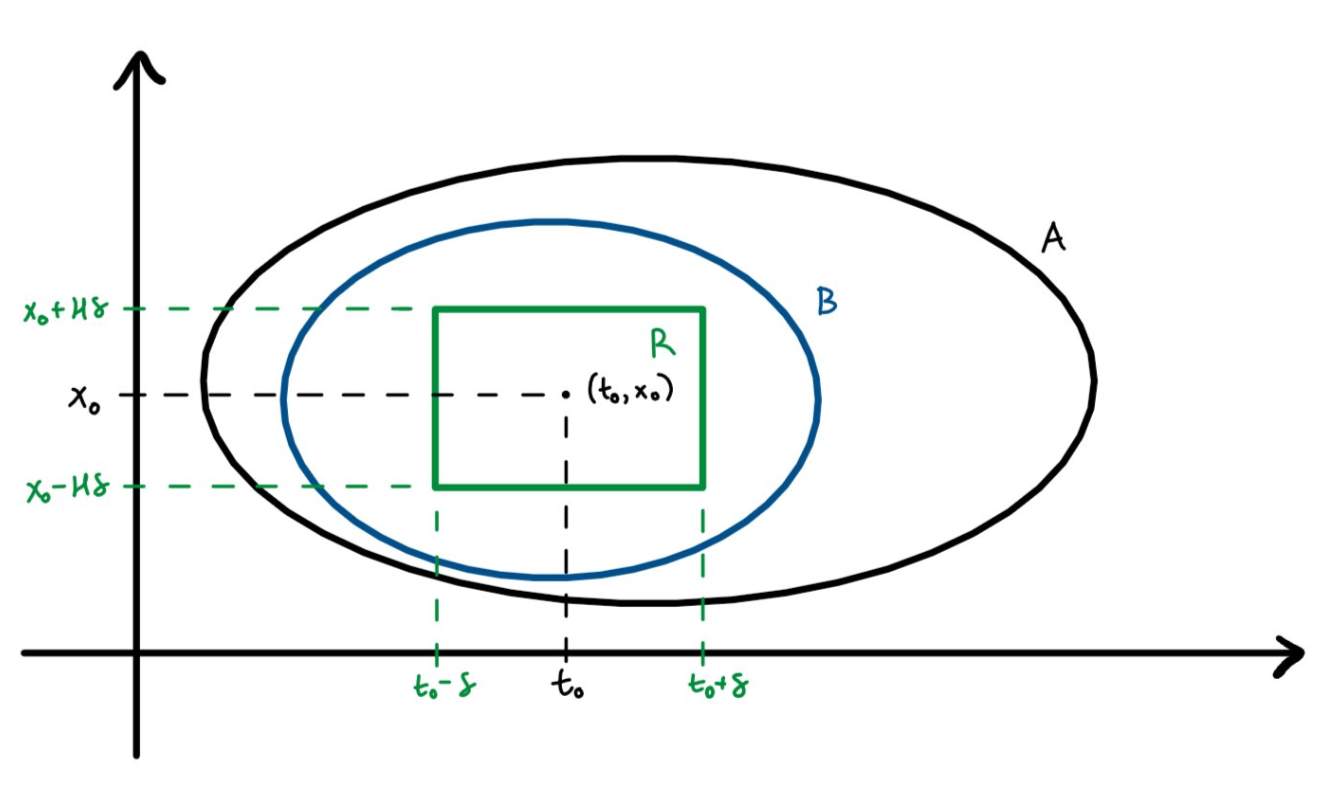
\includegraphics[scale=0.3]{picard}
		\caption{Esquema de la demostración.}
	\end{figure}
	
	Definimos el conjunto:
	 \[X=\{\varphi : I=[t_0-\delta, t_0+\delta]\longrightarrow \mathbb{R}^n : \varphi \text{ continua, } ||\varphi(t)-x_0||\leq H \delta \hspace{0,2cm} \forall t \in I  \} \]
	de las aplicaciones continuas cuyo grafo está en $R$. Dotaremos a este conjunto $ X $ con la siguiente métrica. Dadas $\varphi, \psi \in X$, $d(\varphi, \psi) = sup_{t \in I} \norm{\varphi (t) - \psi (t)}$ (como ejercicio probar que es una métrica). Así tenemos que:\\
	\[\begin{rcases}
		C(I, \mathbb{R}^n) \text{ espacio métrico completo \footnotemark}\\
		X = B_{C(I, \mathbb{R}^n)} [x_0, H\delta] \subset C(I, \mathbb{R}^n) \text{ cerrado } \\
	\end{rcases} \Rightarrow (X, d) \text{ completo.}\]
	\footnotetext{Un espacio métrico completo es aquel en el que toda sucesión de Cauchy converge a un punto en el mismo conjunto. En la demostración usamos el siguiente resultado: Un subconjunto cerrado de un espacio métrico completo es completo.}
	
	Nótese que $ x_0 $ puede ser entendido como la función constante $ x_0 $, en el contexto de un espacio de funciones. Definimos ahora:
	\[T:\varphi \in X \longrightarrow T\varphi = x_0 + \int_{t_0}^{t} f(s, \varphi(s))ds\]
	Queremos usar el Teorema \ref{transformada} de la transformada contractiva, por tanto, tenemos que demostrar:
	\begin{enumerate}
		\item $T\varphi \in X$.
		\item $T$ es $\lambda$-contracción.
	\end{enumerate}
	Para ver que $T\varphi \in X$ tenemos que ver:
	\begin{enumerate}[	i.]
		\item $T\varphi$ continua
		\item $\norm{T\varphi (t) - x_0} \leq H\delta$, $\forall t \in I$
	\end{enumerate}
	En primer lugar, tenemos que:
	\[s \stackrel{g}{\longrightarrow} (s, \varphi (s)) \stackrel{f}{\longrightarrow} f(s, \varphi (s)) \longrightarrow x_0 + \int_{t_0}^{t}f(s,\varphi (s))ds  \]
	por lo que $T\varphi$ es continua por composición de funciones continuas. \\
	En segundo lugar, 
	\[\norm{T\varphi - x_0} = \norm{x_0 + \int_{t_0}^{t} f(s, \varphi (s)) ds - x_0} = \norm{\int_{t_0}^{t} f(s, \varphi (s)) ds} \leq \]
	\[\abs{\int_{t_0}^{t} \norm{f(s, \varphi (s))}ds} \leq \abs{\int_{t_0}^{t} H ds} = \abs{H(t - t_0)} = H\abs{t - t_0} \leq H\delta \]
	Veamos ahora que $T$ es una $\lambda$-contracción, es decir, $\exists \lambda \in \mathbb{R}$, $0 \leq \lambda < 1$ tal que
	\[d(T\varphi, T\psi) \leq \lambda d(\varphi, \psi) \hspace{0,2cm} \forall \varphi, \psi \in X\]
	Sean $\varphi, \psi \in X$, \\
	\[d(T\varphi, T\psi) = sup_{t \in I} \norm{T\varphi (t) - T\psi (t)} = sup_{t \in I} \norm{x_0 + \int_{t_0}^{t} f(s, \varphi(s))ds - x_0 - \int_{t_0}^{t} f(s, \psi(s))ds} = \]
	\[sup_{t \in I} \norm{\int_{t_0}^{t} (f(s, \varphi(s)) - f(s, \psi(s)))ds} \leq sup_{t \in I} \abs{\int_{t_0}^{t} \norm{(f(s, \varphi(s)) - f(s, \psi(s)))}ds} \stackrel{f \in L_{loc} (A, x)}{\leq} \] 
	\[sup_{t \in I} \abs{\int_{t_0}^{t} k\norm{\varphi(s) - \psi(s)}ds} \leq sup_{t \in I} \abs{\int_{t_0}^{t} k sup\norm{\varphi(s) - \psi(s)}ds} \leq sup_{t \in I} \abs{\int_{t_0}^{t} k d(\varphi, \psi)ds} = \]
	\[sup_{t \in I} kd(\varphi, \psi)\abs{t - t_0} \leq kd(\varphi, \psi)\delta \leq \lambda d(\varphi, \psi)\]
	Tomando $\lambda = \delta k$, como $\delta < \frac{1}{k}$ tenemos que $\lambda < 1$. Nótese que podemos aplicar que $ f $ es $ L_{\text{loc}} $ en $ A $ respecto de $ x $ ya que al ser $ \psi $ y $ \varphi $ funciones de $ X $, están definidas en un entorno de $ t_0 $ en el que $ f $ es lipschitziana, y siempre trabajamos con $ t $ dentro de ese entorno, por como estamos construyendo la prueba.
	
	Por lo tanto, $T$ es $\lambda$-contracción. Es decir, por el Teorema \ref{transformada} de la transformada contractiva:
	\[\exists ! \varphi \in X : \varphi \text{ punto fijo de } T\]
	por lo que $\varphi (t) = T\varphi (t) = x_0 + \int_{t_0}^{t} f(s, \varphi (s))ds$, y como $\varphi$ continua, cumple las dos hipótesis del Teorema \ref{carac-sol} de caracterización de soluciones.	

	\begin{figure}[h]
		\centering
		\begin{tikzpicture}
		\draw[->] (-1,0) -- (5,0) node[right] {$t \in \mathbb{R}$}; %eje x, en este caso t
		\draw[->] (0,-0.5) -- (0,3.5) node[above] {$x \in \mathbb{R}^n$};% eje y
		\draw  plot[tension=.7] coordinates {(1,1) (1,2.5) (4,2.5) (4,1) (1,1) }; %conjunto R
		\draw  plot[scale=0.53,shift={(4.3,2.75)},smooth, tension=.7] coordinates {(-3.5,0.5) (-3,2.5) (-1,3.5) (1.5,3) (4,3.5) (5,2.5) (5,0.5) (2.5,-2) (0.5,-1.5) (-3,-2) (-3.5,0.5)}; % conjunto A
		\draw[-] (2.5,0.10) -- (2.5,-0.10) node[below][scale=0.8]{$t_0$}; %t0 y puntos de x
		\draw[-] (1,0.10) -- (1,-0.10) node[below][scale=0.8]{$t_0-\delta$};
		\draw[-] (4,0.10) -- (4,-0.10) node[below][scale=0.8]{$t_0+\delta$};
		\draw[-] (-0.10,1.75) -- (0.10,1.75) node[left=2mm][scale=0.8]{$x_0$}; %x_0 y puntos de y
		\coordinate[label=above:A] (A) at (5.2,2.8); %etiqueta de A
		\coordinate[label=above:R] (R) at (4.2,2.2); %etiqueta de R
		\draw  plot[smooth,tension=.7] coordinates {(1,1.75) (1.5,2.2) (1.7,2) (2.25,2.6) (2.8,0.75) (3.2, 2.6) (3.4, 1.9) (4, 2.3)}; %linea poligonal
		\fill (2.5,1.75)  circle[radius=1pt]; %punto en t0,x_0
		\coordinate[label={[scale=0.6] right:$(t_0,x_0)$}] (p0) at (2.5,1.7); %etiqueta de t0 x0
		\end{tikzpicture}
		\caption{Situación en la que el grafo no está en $ R $.} \label{M1}
	\end{figure}
	¿Podría existir una función que fuera solución pasando por el punto y que el grafo no esté en $ R $? Probemos que no.
	\begin{adjustwidth}{1cm}{}
		Veamos que si $ \psi : I \longrightarrow\mathbb{R}^n $ solución de $ x'=f(t,x) $ pasando por $ (t_0,x_0) $, entonces $ \psi \in X $, es decir, $ ||\psi(t)-x_0||\leq H\delta \ \forall t \in I $.
		
		Probémoslo por reducción al absurdo. Supongamos que $ \exists t_1\in I : ||\psi(t_1)-x_0||>H\delta$, por ser $ \psi $ continua $ \exists t_2\in (t_0,t_1) $ en el cual $ ||\psi(t_2)-x_0||=H\delta $.
		
		Sea $ t^* = \inf \{t : ||\psi(t)-x_0||=H\delta, t>t_0 \} \Rightarrow ||\psi(t^*)-\psi(t_0)||=H\delta$, con $ \psi(t_0)=x_0 $.
		
		Por otra parte, $ ||\psi(t^*)-\psi(t_0)||\leq ||\psi'(t)||\cdot |t^*-t_0|<H\delta $, lo cual es una contradicción.
	\end{adjustwidth}
	
	¿Podría existir otra solución distinta que pasase por el punto?
	\begin{adjustwidth}{1cm}{}
		Veamos que esto tampoco puede pasar. Supongamos que $ \varphi_1: I_1\longrightarrow\mathbb{R}^n, \varphi_2:I_2 \longrightarrow \mathbb{R}^n $ son soluciones de $ x'=f(t,x) $ pasando por $ (t_0,x_0) $ y $ \exists t\in I_1\cap I_2 : \varphi_1(t)\neq \varphi_2(t) $.
		
		Sea por ejemplo $ t>t_0 $. Sea $ t_1=\inf \{t \in I_1\cap I_2 :t>t_0, \varphi_1(t)\neq \varphi_2(t)  \} $.
		
		Por definición de ínfimo $ \varphi_1(t)=\varphi_2(t) \ \forall t \in [t_0, t_1) $ y además $ \varphi_1(t_1)=\lim\limits_{t\to t_1^-} \varphi_1(t) $ por ser $ \varphi_1 $ continua.
		
		$ \varphi_1(t_1)=\lim\limits_{t\to t_1^-} \varphi_1(t)=\lim\limits_{t\to t_1^-} \varphi_2(t)= \varphi_2(t_1) $.
		
		Entonces $ \varphi_1(t)=\varphi_2(t) \ \forall t \in [t_0,t_1], \varphi_1(t_1)=\varphi_2(t_1)=x_1 $.
		
		Hacemos en $ (t_1, x_1) $ lo mismo que en $ (t_0,x_0) $ (construimos el rectángulo, etc...) y llegamos a que en $ (t_1-\delta_1, t_1+\delta _1), \varphi_1(t)=\varphi_2(t) $ y esto NO es posible ya que, por construcción, $ t_1=\inf \{t\in I_1\cap I_2 : t>t_0, \varphi_1(t)\neq \varphi_2(t)\} $.
	\end{adjustwidth}
\end{proof}

\section{Tema 3.}
\begin{example}
	Dada la ecuación diferencial $ x'=x^2 $, pasando por el punto $ x(1)=1 $, tenemos que $ x(t)=\frac{-1}{t} $ es solución. $ x'(t)=x(t)^2 $ es una ecuación planteada para todo $ t \in \mathbb{R} $, pero $ x(t)=\frac{-1}{t} $ está definida para $ t \in \mathbb{R}-\{0\} $.
	
	Entonces tenemos que dependiendo de las condiciones iniciales la solución de la EDO estará definida para $ t\in (0,\infty) $ o $ t\in (-\infty,0) $.
	
	Fijémonos en dos aspectos: con las condiciones iniciales propuestas, $ x(1)=1 $, podemos definir la solución en el intervalo $ (0,3) $. Sin embargo, esta solución podría ser prolongada a un dominio de $ (0,\infty) $, y la posibilidad de esta prolongación será objeto de estudio.
	
	Por otra parte, vemos que al cambiar las condiciones iniciales (por ejemplo, $ x_0=-0.0001 $ o $ x_0=0.00001 $), la solución de la ecuación no es la misma y en otros caso, podría variar su expresión analítica. Nos interesará que para variaciones ''pequeñas'' de las condiciones iniciales, la solución de la ecuación no varíe ''casi nada''.
\end{example}

\begin{note}
	Los teoremas de Cauchy-Peano y Picard-Lipschitz definen existencia y unicidad de soluciones a nivel local, en un entorno arbitrariamente pequeño. Son preguntas naturales: \begin{itemize}
		\item ¿Cuál es el mayor intervalo en el que están definidas esas soluciones?
		\item ¿Hasta donde puedo prolongar las mismas?
	\end{itemize}
\end{note}
\subsection{Prolongación de soluciones. Soluciones maximales.}
\begin{definition}
	Sean $ A $ un abierto de $ \mathbb{R}^{n+1} $ y $ f $ la aplicación continua $ f:(t,x)\in A\subset \mathbb{R}\times \mathbb{R}^n \longrightarrow f(t,x)\in \mathbb{R}^n $, con $  x'=f(t,x) $ su ecuación diferencial asociada. 
	
	Sean además $ \varphi_1:I_1\longrightarrow \mathbb{R} $ y  $ \varphi_2:I_2\longrightarrow \mathbb{R} $ soluciones de dicha ecuación diferencial. Diremos que $ \varphi_2 $ es una \iindex{prolongación} de $ \varphi_1 $ si:
	\begin{enumerate}
		\item $ I_1\subseteq I_2 $
		\item $ \varphi_1(t) =\varphi_2(t) \ \forall t \in I_1$
	\end{enumerate}

	Además, si $ I_1 \varsubsetneq I_2 $ diremos que $ \varphi_2 $ es una \iindex{prolongación propia} de $ \varphi_1 $.
\end{definition}
\begin{note}
	Una solución es prolongación de si misma, pero no es prolongación propia.
\end{note}
\begin{definition}
	Si $ \varphi $ es solución de una ecuación diferencial, diremos que $ \varphi $ es una \iindex{solución maximal} si no admite prolongación propia. En este caso, el intervalo de definición es llamado \iindex{intervalo maximal}.
\end{definition}
\begin{lemma}[Lema de Zorn]
	Todo conjunto parcialmente ordenado no vacío, en el que toda cadena (subconjunto parcialmente ordenado) admite cota superior, contiene elementos maximales.
\end{lemma}
\begin{theorem}
	Sean $ A $ un abierto de $ \mathbb{R}^{n+1} $ y $ f $ la aplicación continua $ f:(t,x)\in A\subset \mathbb{R}\times \mathbb{R}^n \longrightarrow f(t,x)\in \mathbb{R}^n $, con $  x'=f(t,x) $ su ecuación diferencial asociada. 
	
	Dado $ (t_0,x_0)\in A $, existe una solución maximal de la ecuación diferencial que pasa por $ (t_0,x_0) $.
	
\end{theorem}
\begin{proof} \ \\	
	Haremos uso del lema de Zorn. Representaremos las soluciones de la ecuación diferencial mediante el par $ (I,\varphi) $ donde $ \varphi $ es la solución e $ I $ su intervalo de definición.
	
	En este conjunto definimos la relación de orden parcial "ser prolongación". Si $ \psi $ es prolongación de $ \varphi $:
	\[ (I,\varphi)\leq (J,\psi)\Leftrightarrow I\subseteq J, \varphi(t)=\psi(t) \ \forall t \in I \]
	Ahora, sea $ (I_0,\varphi_0) $ solución de $ x'=f(t,x) $ y veamos que se puede prolongar hasta una solución maximal.
	
	Trabajamos solo con soluciones que sean prolongación de $ \varphi_0 $. Es un conjunto no vacío, ya que $ (I_0,\varphi_0) $ es prolongación de si mismo. Utilizamos la relación de orden parcial definida anteriormente y comprobamos que se cumple la otra hipótesis del lema de Zorn:
	
	Sea $ \{(I_j,\varphi_j) \}_{j\in I} $ una cadena de ese conjunto y veamos que admite cota superior. Sea $ \varphi $ la función definida en $ I=\bigcup_{j\in I}I_j $ mediante $ \varphi(t)=\varphi_j(t) \ \forall j \in I $. $ \varphi $ es claramente cota superior de la cadena.
	
	Por tanto, por el lema de Zorn, existen elementos maximales que son las soluciones maximales que prolongan a $ \varphi_0 $.	
\end{proof}
\begin{definition}
	Sean $ A $ un abierto de $ \mathbb{R}^{n+1} $ y $ f $ la aplicación continua $ f:(t,x)\in A\subset \mathbb{R}\times \mathbb{R}^n \longrightarrow f(t,x)\in \mathbb{R}^n $, con $  x'=f(t,x) $ su ecuación diferencial asociada. 
	
	Sean $ \varphi_1:(a,b)\longrightarrow \mathbb{R}^n $ y $ \varphi_2:(c,d)\longrightarrow \mathbb{R}^n $ soluciones de dicha ecuación diferencial. Si $ \varphi_2 $ es una prolongación de $ \varphi_1 $ y $ b\in(c,d) $, diremos que $ \varphi_2 $ es \iindex{prolongación de $ \varphi_1 $ a través de $ b $}.
\end{definition}
\begin{definition}[General]
	Sean $ A $ un abierto de $ \mathbb{R}^{n+1} $ y $ f $ la aplicación continua $ f:(t,x)\in A\subset \mathbb{R}\times \mathbb{R}^n \longrightarrow f(t,x)\in \mathbb{R}^n $, con $  x'=f(t,x) $ su ecuación diferencial asociada. 
	
	Sean $ \varphi_1:I_1\longrightarrow \mathbb{R}^n $ y $ \varphi_2:I_2\longrightarrow \mathbb{R}^n $ soluciones de dicha ecuación diferencial. Si $ \varphi_2 $ es una prolongación de $ \varphi_1 $ y existe $ q\in \text{Fr}(I_1) $ tal que $ q\in \mathring{I_2}$, diremos que $ \varphi_2 $ es \iindex{prolongación de $ \varphi_1 $ a través de $ q $}.
\end{definition}
\begin{theorem}[Teorema de prolongación] \label{prolTh}
	Sean $ A $ un abierto de $ \mathbb{R}^{n+1} $ y $ f $ la aplicación continua $ f:(t,x)\in A\subset \mathbb{R}\times \mathbb{R}^n \longrightarrow f(t,x)\in \mathbb{R}^n $, con $  x'=f(t,x) $ su ecuación diferencial asociada. 
	
	Además de estas condiciones habituales, pediremos que $ f\in L_{\text{loc}}(A,x) $, es decir, que $ f $ sea lipschitziana localmente.
	
	Si $ \varphi:(a,b)\longrightarrow\mathbb{R}^n $ es solución de la ecuación diferencial anterior, entonces;
	\begin{enumerate}[\quad i)]
		\item $ \varphi $ prolongable a través de $ b \Leftrightarrow \exists \lim\limits_{t\to b^-}\varphi(t)=p, \text{ con } (b,p) \in A $
		\item $ \varphi $ prolongable a través de $ a \Leftrightarrow \exists \lim\limits_{t\to a^+}\varphi(t)=q, \text{ con } (a,q) \in A $
	\end{enumerate}
\end{theorem}


\begin{proof}\ 
	\begin{enumerate} [\quad i)]
		\item "$\Rightarrow$" \\
		Si $\varphi$ prolongable a través de $b$, entonces $\exists \varphi_2 : (a, d) \longrightarrow \mathbb{R}^n$ prolongación de $\varphi$ (es decir, $\varphi_2 = \varphi$ $\forall t \in (a, b)$, $b \in (a, b)$). Por ser $\varphi_2$ solución, $\varphi_2$ es continua por la izquierda en $t = b$, por lo que:
		\[\lim\limits_{t \to b^-} \varphi_2(t) = \varphi_2(b) \text{, } \lim\limits_{t \to b^-} \varphi_2(t) = \lim\limits_{t \to b^-} \varphi(t)\]
		y tenemos entonces que:
		\[\lim\limits_{t \to b^-} \varphi(t) = \varphi_2(b)\]
		Además, $(b, \varphi(b)) \in A$ por ser $\varphi_2$ solución. \\
		"$\Leftarrow$" \\
		Suponemos que:
		\[\exists \lim\limits_{t \to b^-} \varphi(t) = p \text{, } (b, p) \in A\]
		Sea $\overline{B} = B((b, p), r) \subset A$ con $f$ acotada en $\overline{B}$ y $f \in L_k (B, x)$. Tomamos $0 < \delta < min\{\frac{r}{2}, \frac{r/2}{H}, \frac{1}{k}\}$, siendo $H$ cota de $f$.
		
		\begin{figure}[h]
			\centering
			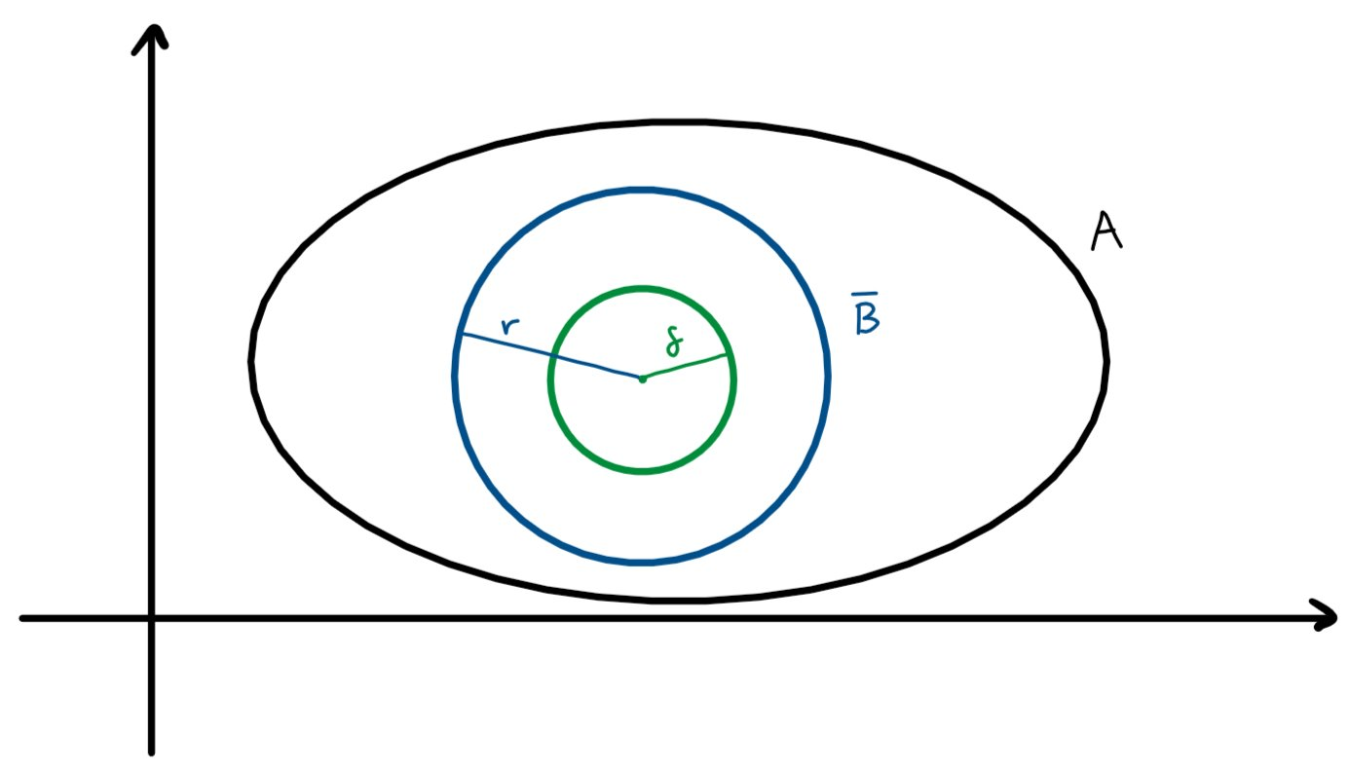
\includegraphics[scale=0.3]{prolongacion}
			\caption{Conjuntos implicados.}
		\end{figure}
		
		Como $\lim\limits_{t \to b^-} \varphi (t) = p$ y, por ser continua, $ \varphi $ es secuencialmente continua, existe una sucesión $\{t_n\} \longrightarrow b^-$ tal que $\{\varphi(t_n)\} \longrightarrow p$. Elegimos entonces un $n_0 \in \mathbb{N}$ tal que $\abs{t_{n_0} - b} < \delta$ y $(t_{n_0}, \varphi (t_{n_0})) \in \overline{B}$. Para la condición inicial $(t_{n_0}, \varphi (t_{n_0}))$ existe una solución única pasando por el punto definido en $[t_{n_0} - \delta, t_{n_0} + \delta]$ que denoto $\overline{\varphi}$. Entonces la función:
		\[\psi: (a, t_{n_0} + \delta] \longrightarrow \psi (t) = \begin{cases}
		\varphi(t) &t \in (a, b) \\ 
		\overline{\varphi} (t) &t \in [b, t_{n_0} + \delta).
		\end{cases}\]
		Así, tenemos que $\psi$ es solución de $x' = f(t. x)$ y, de hecho, $\psi$ prolonga a $\varphi$ a través de $b$.
		\item Análogo.
	\end{enumerate} 
\end{proof}
\begin{observation}
	En primer lugar, la afirmación $i)$ es equivalente a decir:
	\[\exists \{t_m\} \longrightarrow b^- : \exists \lim\limits_{t_n \to b^-} \varphi(t_n) = p \hspace{0.2cm} (b, p) \in A\]
	Llega trabajar con una sucesión. Además, no es necesario pedir que $f \in L_{loc}(A, x)$, simplemente sin ella no podemos concluir la unicidad y la demostración sería mucho más complicada.
\end{observation}
\begin{corollary}
	Si $A$ está acotado, la solución se puede prolongar hasta la frontera.
\end{corollary}
\begin{theorem}[Teorema de la banda]\label{banda} \ \\ 
	Dada la ecuación diferencial $x' = f(t, x)$, con $f: (t, x) \in \mathbb{R} \times \mathbb{R}^n \longrightarrow f(t, x) \in \mathbb{R}^n$ siendo $A = (a, b) \times \mathbb{R}^n$. Si se cumple una de las siguientes condiciones:
	\begin{enumerate}
		\item  $f$ continua en $A$, $f \in L_k (A, x)$.
		\item  $f$ continua y acotada en $A$ ($f \in L_{loc} (A, x)$).
	\end{enumerate}
	
	\begin{figure}[h]
		\centering
		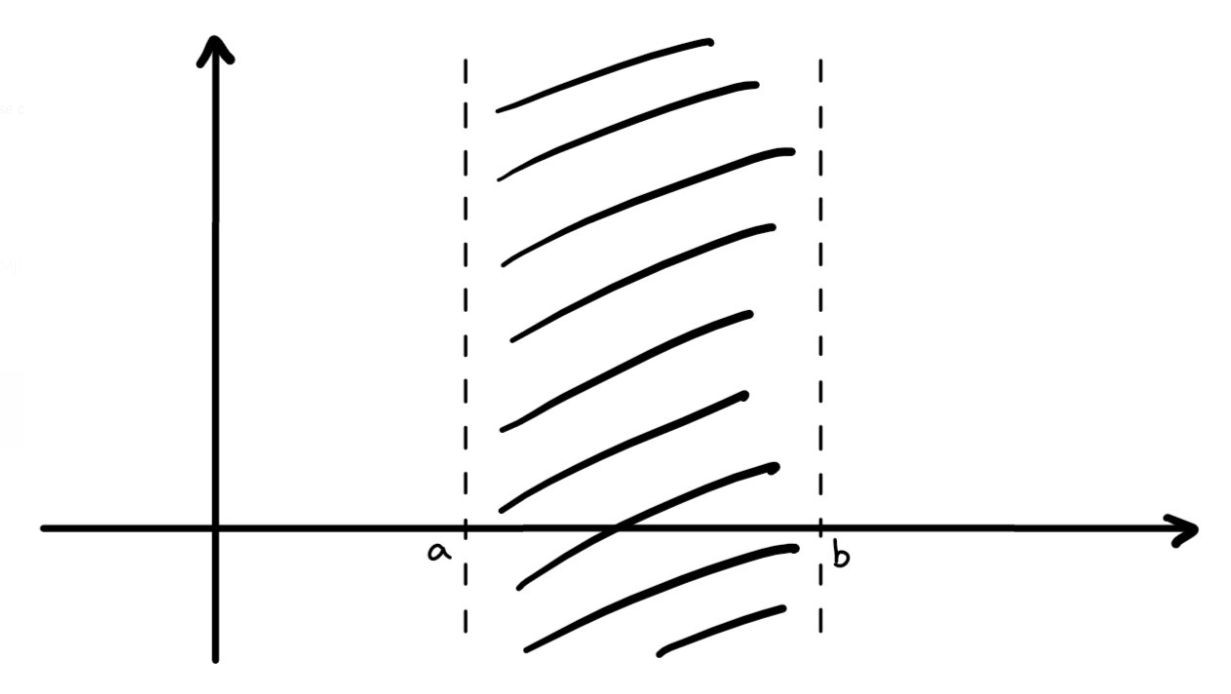
\includegraphics[scale=0.3]{banda}
		\caption{Teorema de la banda.}
	\end{figure}
	
	entonces, fijado $(t_0, x_0) \in (a, b) \times \mathbb{R}^n$, la solución maximal que pasa por él está definida en $(a, b)$.
\end{theorem}
\begin{observation} \ 
	\begin{enumerate}
		\item No es necesario pedir $f \in L_{loc} (A, x)$.
		\item $a$, $b$ no tienen porque ser finitos, es decir, puede tratarse de intervalos de la forma $(- \infty, b)$.
	\end{enumerate}
\end{observation}
\begin{theorem}[Teorema de la banda cerrada] \label{bandacerrada} \ \\
	Dada la ecuación diferencial $x' = f(t, x)$, con $f: [a, b] \times \mathbb{R}^n \longrightarrow \mathbb{R}^n$. Si se cumple una de las siguientes condiciones:
	\begin{enumerate}
		\item $f$ continua en $A = [a, b] \times \mathbb{R}^n$, $f \in L_k (A, x)$.
		\item $f$ continua en $A$, $f \in L_{loc} (A, x)$.
	\end{enumerate}
	entonces, fijado $(t_0, x_0) \in A$ la solución maximal pasando por ese punto está definida en $[a, b]$. 
\end{theorem}
\begin{proof}\ \\
	Definimos la siguiente función, donde $A \subset (c, d) \times \mathbb{R}^n$:
	\[g: (t, x) \in (c, d) \times \mathbb{R}^n \longrightarrow g(t, x) = \begin{cases}
	f(a, x), &t \in (c, a] \\
	f(t, x), &t \in [a, b] \\
	f(b, x), &t \in [b, d)
	\end{cases}\]
	y con $g$ continua. Esta función verifica las hipótesis del teorema anterior en $(c, d) \times \mathbb{R}^n$ ya que:
	\begin{enumerate}[-]
		\item Si $f \in L_k(A, x) \Rightarrow g \in L_k ((c, d) \times \mathbb{R}^n)$
		\item Si $f$ acotado y $f \in L_{loc} (A, x)$, entonces $g$ acotada y $g \in L_{loc} ((c, d) \times \mathbb{R}^n, x)$.
	\end{enumerate}
	Por tanto, fijado $(t_0, x_0) \in A \subset (c, d) \times \mathbb{R}^n$ existe la solución maximal pasando por $(t_0, x_0)$ y definida en $(c, d)$. Por tanto, $\varphi = \psi|_{[a, b]}$ es la solución maximal de $x' = f(t, x)$ pasando por $(t_0, x_0)$.
	
	\begin{figure}[h]
		\centering
		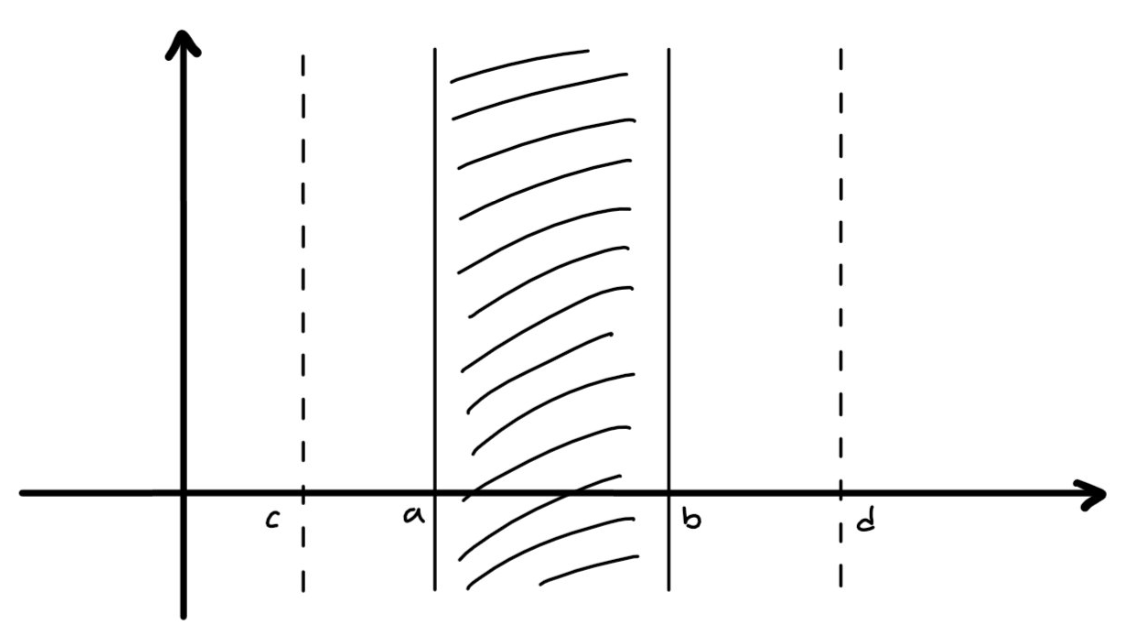
\includegraphics[scale=0.3]{banda_cerrada}
		\caption{Teorema de la banda cerrada.}
	\end{figure}
	\end{proof}

\begin{proposition}
	Sean $ A $ un abierto de $ \mathbb{R}^{n+1} $ y $ f $ la aplicación continua $ f:(t,x)\in A\subset \mathbb{R}\times \mathbb{R}^n \longrightarrow f(t,x)\in \mathbb{R}^n $, con $  x'=f(t,x) $ su ecuación diferencial asociada. 
	
	Si $ \varphi_1, \varphi_2 $ son soluciones de la ecuación, definidas en $ [a, t_0]$ y $ [t_0,b] $, respectivamente, y además $ \varphi_1(t_0)=\varphi_2(t_0) $, entonces $ \varphi $ definida en $ [a,b] $ como:
	\[ \varphi(t)=\begin{cases}
	\varphi_1(t), \quad t\in [a,t_0]\\
	\varphi_2(t), \quad t\in [t_0,b]
	\end{cases} \]
	es solución de la ecuación diferencial.
\end{proposition}
\begin{proof}\ \\
	Veamos que $ \varphi $ es solución por definición:
	\begin{enumerate}[\quad i)]
		\item $ (t,\varphi(t))\in A \ \forall t \in [a,b], $ ya que $ \begin{cases}
		\forall t\in [a,t_0] \quad (t, \varphi_1(t)) \in A, \text{ ya que }\varphi_1 \text{ es solución.}\\
		\forall t\in [t_0,b] \quad (t, \varphi_2(t)) \in A, \text{ ya que }\varphi_2 \text{ es solución.}\\
		\text{Además, } \varphi_1(t)=\varphi_2(t).
		\end{cases}$
		\item $ \forall t \in [a,t_0) \ \exists \varphi_1'(t)$
		
		$ \forall t \in [t_0,b) \ \exists \varphi_2'(t) $
		
		Veamos si existe la derivada en $ t_0 $, utilizando la continuidad de $ \varphi_1 $ y $ \varphi_2 $:
		\[ \lim\limits_{t \to t_0^-} \varphi'_1(t)=\lim\limits_{t \to t_0^-} f(t, \varphi_1(t))=f(t_0,\varphi_1(t_0)) \]
		\[ \lim\limits_{t \to t_0^+} \varphi'_2(t)=\lim\limits_{t \to t_0^+} f(t, \varphi_2(t))=f(t_0,\varphi_2(t_0)) \]
		Como $ \varphi_1(t_0)=\varphi_2(t_0) \Rightarrow \lim\limits_{t \to t_0^-} \varphi'(t)=\lim\limits_{t \to t_0^+} \varphi'(t)$, y $\varphi $ continua en $ t_0 $, entonces efectivamente existe $ \varphi'(t_0) $.
		\item Inmediata visto lo anterior.
	\end{enumerate} 
\end{proof}
\begin{proposition}
	Sean $ A $ un abierto de $ \mathbb{R}^{n+1} $ y $ f $ la aplicación continua $ f:(t,x)\in A\subset \mathbb{R}\times \mathbb{R}^n \longrightarrow f(t,x)\in \mathbb{R}^n $, con $  x'=f(t,x) $ su ecuación diferencial asociada. 
	
	Entonces, toda solución maximal está definida en un abierto.
\end{proposition}
\begin{proof}\ \\
	Probémoslo por reducción al absurdo. Supongamos que está definida en un intervalo de la forma $ (a,b] $.
	Como $ A $ es abierto, $ (b,\varphi(b))\in A \Rightarrow (b, \varphi(b)) \in \mathring{A} $.
	
	Estamos en la hipótesis del Teorema de Cauchy-Peano. Por lo tanto, pasando por $ (b, \varphi(b)) $ existe solución. Podemos construir una prolongación que sea solución (por el teorema \ref{prolTh} apartado i) y entonces no es maximal.
\end{proof}


\section{Tema 4.}
\subsection{Métodos elementales de integración de las ecuaciones de primer orden.}
\subsubsection{EDOs de variables separadas.}
Son ecuaciones de la forma $ x'=\frac{\partial x}{\partial t}=h(t)g(x) $, con $ h:I_1\longrightarrow\mathbb{R} $ y $ g:I_2\longrightarrow\mathbb{R} $ continuas. 
\paragraph{Justificación de existencia y unicidad de la solución} \ \\
Como $ A=I_1\times I_2 $ debe ser abierto, los intervalos deben ser abiertos. Por la continuidad de $ h $ y $ g $ se deduce la continuidad de $ f(t,x)=h(t)g(x) $, lo que nos permite aplicar el teorema \ref{cauchy-peano} de existencia de solución.

Si además queremos la unicidad de la misma, necesitamos que $ f $ sea localmente lipschitziana respecto a $ x $ para poder aplicar el teorema \ref{picard}, es decir, que $ g $ sea localmente lipschitziana respecto a $ x $. Tal y como vimos en el teorema \ref{lloc_suf}, es suficiente que $ g\in C'(I_2) $.

En estas condiciones, fijado $ (t_0,x_0)\in I_1\times I_2=A $, comprobemos que cumplimos las hipótesis del teorema \ref{picard}:
\begin{enumerate}[i)]
	\item $ I_1\times I_2 $ abierto.
	\item $ f(t,x)=h(t)g(x) $ continua por producto de funciones continuas.
	\item $ f\in L_{loc} (A,x) $ ya que $ g\in L_{loc}(I_2,x) $
\end{enumerate}

\paragraph{Método de resolución}
\begin{enumerate}
	\item $ \frac{1}{g(x)}\cdot\frac{\partial x}{\partial t}=h(t) $
	\item $ \frac{1}{g(x)}\cdot\partial x=h(t)\partial t $
	\item $ \int \frac{1}{g(x)} \partial x= \int h(t) \partial t \Rightarrow G(x)+c_1=H(t)+c_2 \Rightarrow G(x)=H(t)+c$
\end{enumerate}
Si se pide la solución pasando por $ (t_0,x_0) $, hallamos la $ c $ que cumple $ G(x_0)=H(t_0)+c $, es decir, $ G(x)=H(t)+G(x_0)-H(t_0) \Rightarrow G(x)-G(x_0)=H(t)-H(t_0)$.

Otra forma de llegar a este resultado es observar:
\[ \int_{x_0}^{x} \frac{1}{g(x)} \partial x= \int_{t_0}^{t} h(t) \partial t \Rightarrow G(x)-G(x_0)=H(t)-H(t_0)\]

Nótese que si $ g(x_0)=0 $, entonces $ x(t)=x_0 $ es la solución.

\paragraph{Justificación de que la solución está bien definida}
\begin{theorem}
	Sea $ M:(t,x)\longrightarrow M(t,x)=G(x)-G(x_0)-(H(t)-H(t_0)) $. Entonces $ M(t,x) $ define implícitamente una solución de $ x'=f(t,x)=h(t)g(x) $, es decir, la expresión obtenida en el método de resolución es correcta y la solución viene dada por $ M(t,x)=0 $.
\end{theorem}
\begin{proof}
	Probémoslo utilizando el teorema de la implícita. Nótese que 
	\[  M(t,x)=G(x)-G(x_0)-(H(t)-H(t_0))= \int_{x_0}^{x} \frac{1}{g(x)} \partial x- \int_{t_0}^{t} h(t) \partial t \]
	Comprobamos las hipótesis:
	\begin{enumerate}
		\item $ M\in C'(A) $, ya que $ h $ y $ g $ continuas.
		\item $ M(t_0,x_0)=0 $
		\item $ \frac{\partial M}{\partial x}(t_0,x_0)=\frac{1}{g(x_0)}\neq 0 $.
	\end{enumerate}
	Como se cumplen las hipótesis, el teorema de la implícita nos asegura que existen $ \varepsilon_{t_0} $ entorno de $ t_0 $, $ \varepsilon_{x_0} $ entorno de $ x_0 $ y $ x:t\in\varepsilon_{t_0}\longrightarrow x(t)\in\varepsilon_{x_0}$. Además, nos dice que $ x(t) $ cumple:
	\begin{enumerate}
		\item $ x $ continua en el entorno.
		\item $ x(t_0)=x_0 $.
		\item $ M(t,x(t))=0 $ para todo $ t\in \varepsilon_{t_0} $, y $ x(t) $ es la única solución de $ M(t,x(t))=0 $.
		\item $ D x(t)=-[D_x M(t,x(t))]^{-1}D_tM(t,x(t)) $. Es decir:
		\[ Dx(t)=x'(t)=\frac{\partial x}{\partial t}= -[\frac{1}{g(x)}]^{-1}(-h(t))=h(t)g(x)=f(t,x) \]
	\end{enumerate}
	Por lo que efectivamente, la función $ x(t) $ definida implícitamente cumple las condiciones para ser solución de la ecuación diferencial.
\end{proof}
\subsubsection{EDOs homogéneas.}
Son ecuaciones de la forma $ x'=g(\frac{x}{t}), $ o bien $ x'=\frac{f(t,x)}{h(t,x)} $, con $ f,h $ funciones homogéneas del mismo grado.
\begin{definition}
	Decimos que $ f $ es una \iindex{función homogénea de grado $ k $} si $ \forall r \in \mathbb{R}, f(rt,rx)=r^kf(t,x)$.
\end{definition}
\paragraph{Método de resolución} \ \\
Sean $ f,h $ homogéneas del mismo grado. Todas las EDOs homogéneas se pueden reducir a $ x'=g(\frac{x}{t})$.
Reducción de  $ x'=\frac{f(t,x)}{h(t,x)} $, tomando $ r=\frac{1}{t} $:
	\[ x'= \frac{f(t,x)}{h(t,x)}=\frac{(\frac{1}{t})^kf(t,x)}{(\frac{1}{t})^kh(t,x)}=\frac{f((\frac{1}{t})t,\frac{x}{t})}{h((\frac{1}{t})t,\frac{x}{t})}=\frac{f(1,\frac{x}{t})}{h(1,\frac{x}{t})}=g(\frac{x}{t})\]
	Una vez tenemos la ecuación en la forma $ x'=g(\frac{x}{t}) $:
	\begin{enumerate}
		\item $ \frac{x}{t}=u\Rightarrow x=u\cdot t $.
		\item Derivando la expresión anterior respecto a $t,\  x'(t)=u(t)+tu'(t)=g(u) \Rightarrow tu'(t)=g(u)-u(t) $
		\item Resolver $ u'(t)=\frac{g(u)-u}{t} $, que es una EDO de variables separadas en $ u $ y $ t $.
		\item Deshacer el cambio de variable, teniendo en cuenta que $ u=\frac{x}{t} $.
	\end{enumerate}

\subsubsection{EDOs reducibles a homogéneas.}
Son ecuaciones de la forma \[ x'=f(\frac{at+bx+c}{mt+nx+p}) \]con $ a,b,c,m,n,p \in \mathbb{R} $.
\paragraph{Método de resolución} \ \\
Para resolverlas, consideramos la ecuación como el cociente de dos rectas en el plano y razonamos su posición relativa para reducir la ecuación a un tipo ya conocido:
\begin{align*}
r&:at+bx+c=0\\
l&:mt+nx+p=0
\end{align*}
Por casos, ¿las rectas pasan por el origen?:
\begin{enumerate}[\quad i)]
	\item $ c=p=0 $, es decir, las dos pasan por el origen.
	\[ x'=f(\frac{at+bx}{mt+nx})=f(\frac{a+b(\frac{x}{t})}{m+n(\frac{x}{t})}) \text{ homogénea.} \]
	\item $ c $ y $ p $ no son ambos nulos.
	\begin{enumerate}
		\item $ r $ y $ l $ se cortan en otro punto. En el apartado anterior vimos que si se cortaban en otro punto era homogénea. Podemos trasladar los ejes al punto de corte aplicando un cambio de variable y repetir el razonamiento anterior.
		
		\begin{figure}[h]
			\centering
			\begin{tikzpicture}[x=0.75pt,y=0.75pt,yscale=-1,xscale=1]	
			%Shape: Axis 2D [id:dp4031260299087579] 
			\draw[line width=0.75pt]   (163,207.7) -- (333.5,207.7)(180.05,70) -- (180.05,223) (326.5,202.7) -- (333.5,207.7) -- (326.5,212.7) (175.05,77) -- (180.05,70) -- (185.05,77)  ;
			%Straight Lines [id:da2069863440207952] 
			\draw [line width=0.75pt]    (230.5,73) -- (273.5,219) ;
			
			%Straight Lines [id:da7364525271296537] 
			\draw[line width=0.75pt]    (167.5,152) -- (318.5,78) ;
			
			%Shape: Circle [id:dp6288291967071182] 
			\draw  [fill={rgb, 255:red, 0; green, 0; blue, 0 }  ,fill opacity=1 ] (240.83,115) .. controls (240.83,113.8) and (241.8,112.83) .. (243,112.83) .. controls (244.2,112.83) and (245.17,113.8) .. (245.17,115) .. controls (245.17,116.2) and (244.2,117.17) .. (243,117.17) .. controls (241.8,117.17) and (240.83,116.2) .. (240.83,115) -- cycle ;
			
			% Text Node
			\draw (268,123.67) node [scale=0.9] [align=left] {$\displaystyle ( \alpha ,\beta )$};
			% Text Node
			\draw (319,89.67) node  [align=left] {$\displaystyle l$};
			% Text Node
			\draw (229,88.67) node  [align=left] {$\displaystyle r$};
			\end{tikzpicture}
			\caption{Cambio de ejes.}
		\end{figure}
		
		$ (t,x) = (\alpha,\beta)+(s,y) $, por lo que $ \begin{cases}
		t=\alpha+s\\
		s=\beta+y
		\end{cases} $
		
		Además, como \[  x'=\frac{\partial x}{\partial t}=\frac{\partial (\beta+y)}{\partial t}=\frac{\partial y}{\partial s}\frac{\partial s}{\partial t}=\frac{\partial y}{\partial s}   \]tenemos:
		
		\[  x'=\frac{\partial y}{\partial s}= f(\frac{a(\alpha+s)+b(\beta+y)+c}{m(\alpha+s)+n(\beta+y)+p})= f(\frac{as+by+a\alpha+b\beta+c}{ms+ny+m\alpha+n\beta+p})  \]
		Pero como las rectas se cortan en $ (\alpha, \beta) $, tenemos que $ a\alpha+b\beta+c=0 $ y $ m\alpha+n\beta+p=0 $. Es decir:
		\[ x'=f(\frac{as+by}{ms+ny})=f(\frac{a+b(\frac{y}{s})}{m+n(\frac{y}{s})})=g(\frac{y}{s}) \text{ homogénea.}\]
		\item $ r $ y $ l $ son paralelas. En este caso, que sean paralelas quiere decir que $ (a,b)=k(m,n) $, ya que su vector dirección debe ser proporcional. Por lo tanto,
		\[ x'=f(\frac{at+bx+c}{mt+nx+p})=f(\frac{kmt+knx+c}{mt+nx+p})=f(\frac{k(mt+nx)+c}{(mt+nx)+p})\]
		Realizando el cambio de variable $ z=mt+nx $:
		\[ \frac{\partial z}{\partial t}=z'=m+nx'=m+nf(\frac{kz+c}{z+p}) \text{ ecuación de variables separadas.} \]
		Nótese que es necesario deshacer el cambio de variable tras la resolución.
	\end{enumerate}
\end{enumerate}
\subsubsection{EDOs lineales.}
Son ecuaciones de la forma $ x'=a(t)x+b(t) $ con $ a,b: I\in\mathbb{R}\longrightarrow \mathbb{R} $ continuas.
\begin{definition}\ 
	\begin{enumerate}[\quad i)]
		\item Si $ b(t)=0 $, es una \iindex{EDO lineal homogénea}.
		\item Si $ b(t)\neq 0 $, para algún $ t\in I $, es una \iindex{EDO lineal no homogénea o completa}.
	\end{enumerate}
\end{definition}
\paragraph{Método de resolución} \ \\
Distinguiremos según el tipo de ecuación lineal:
\begin{enumerate}[\quad i)]
	\item Ecuación lineal homogénea, $ x'=a(t)x $. Es una ecuación de variables separadas.
	\[ \int\frac{1}{x}dx=\int a(t)dt\Rightarrow\ln\abs{x}=\int a(t)dt+k, \ k\in\mathbb{R}\Rightarrow\abs{x}=e^{k+\int a(t)dt}=k'e^{\int a(t)dt}, \ k'>0 \]
	\[ \abs{x}=\begin{cases}
	\ \ x=k'e^{\int a(t)dt}, \ x>0, k'>0\\
	-x=k'e^{\int a(t)dt}, \ x<0, k'>0
	\end{cases}\Rightarrow x=ce^{\int a(t)dt}, \ c\in \mathbb{R}  \]
	Para hallar una solución particular, sustituyo teniendo en cuenta que $ x(t_0)=x_0 $ y hallo $ c $. Nótese que si $ x_0>0,\ x(t)>0\ \forall t $, ya que al ser $ x(t)= \psi(t)=0 \ \forall t$ una solución de la EDO, si $ x(t)= \varphi(t)\neq0 $ para algún t y existe un $ t_0 $ tal que $ \varphi(t_0)=0 $, tendríamos dos soluciones por $ (t_0,0) $ ($ \psi $ y $ \varphi $), pero las EDOs lineales están en las hipótesis del teorema \ref{picard} de Picard-Lipschitz que nos asegura unicidad de la solución.
	
	Análogamente, si $ x_0<0,\ x(t)<0\ \forall t $.
	\item Ecuación lineal completa, $ x'=a(t)x +b(t) $. Usaremos el método de las variación de constantes. Buscaremos una función $ c(t) $ tal que $ x(t)=c(t)e^{\int a(t) dt} $ sea solución. La justificación formal de porque tiene esta forma la solución se desarrolla en la proposición \ref{ecLinCompleta}.
	
	A partir de este resultado, construimos un método práctico de resolución. Por ser $ x(t) $ solución, ha de verificar $ x'(t)=a(t)x+b(t) $, es decir,
	\[ c'(t)e^{\int a(t)dt}+c(t)e^{\int a(t)dt}a(t)=a(t)c(t)e^{\int a(t)dt}+b(t) \]
	Por tanto, $ c'(t)e^{\int a(t)dt}=b(t) $. Después de reordenar, por ser continua podemos integrar y obtenemos:
	\[ c(t)=\int \frac{b(t)}{e^{\int a(t)dt}}=h(t)+k, \ k\in \mathbb{R} \]
	Por lo que la solución general de la completa será:
	\[ x(t)=(h(t)+k)\cdot e^{\int a(t)dt}=ke^{\int a(t)dt}+h(t)e^{\int a(t)dt} \]
	Es decir, la solución general de la completa será la suma de la solución general de la homogénea con la solución particular de la completa para $ k=0 $.
\end{enumerate}
\paragraph{Justificación de existencia y unicidad de la solución}\ \\
En este caso, $ f(t,x)=a(t)x+b(t) $. Si $ t_0\in I $ intervalo abierto, $ (t_0, x_0)\in I\times \mathbb{R}=A $. Es decir, $ A $ es abierto. Además $ f $ es continua ya que $ a(t) $ y $ b(t) $ son continuas. Como también $ \frac{\partial f}{\partial x}=a(t) $ es continua, tenemos por el teorema \ref{lloc_suf} que $ f\in L{loc}(A,x) $ y por el teorema \ref{picard} de Picard-Lipschitz, existe una solución que pasa por $ (t_0, x_0)\in A$ y es única.

\begin{proposition}\label{ecLinCompleta}
	Sea $ x'=a(t)x $ la ecuación lineal homogénea que tiene solución $ x(t)=c e^{\int a(t) dt} $, con $ c\in \mathbb{R} $ (como vimos en su resolución como ecuación de variables separadas). 
	
	La ecuación lineal completa $ x'(t)=a(t)x+b(t) $ tiene solución de la forma: \[ x(t)= c(t)e^{\int a(t) dt}\text{ , con } c(t)= b(t)e^{-\int a(t) dt}+k\]
\end{proposition}
\begin{proof}
	Queremos encontrar una solución para $ x'(t)=a(t)x+b(t) $. Multiplicamos por $ e^{-\int a(t)dt} $  toda la igualdad.
	\[ x'(t)e^{-\int a(t)dt}=a(t)x(t)e^{-\int a(t)dt}+b(t)e^{-\int a(t)dt}\]
	Reordenando:
	\[  x'(t)e^{-\int a(t)dt}-a(t)x(t)e^{-\int a(t)dt}=b(t)e^{-\int a(t)dt} \]
	Calculamos ahora, por la regla del producto:	
	\[ \begin{split}
	\frac{d}{dt}\left( x(t)e^{-\int a(t)dt}\right) &=x'(t)e^{-\int a)(t)dt}+\frac{d}{dt}\left( e^{-\int a(t)dt}\right) x(t)\\
	&=x'(t)e^{-\int a(t)dt}-a(t)e^{-\int a(t)dt}x(t)\\
	&=b(t)e^{-\int a(t)dt}
	\end{split} \]
	utilizando que $ \frac{d}{dt}e^{-\int a(t)dt}=-a(t)e^{-\int a(t)dt} $ y el término reordenado de arriba.
	Ahora, integramos para obtener la solución general:
	\[ \frac{x(t)}{e^{\int a(t)dt}}+k= \int b(t)e^{-\int a(t)dt} dt\Rightarrow x(t)= \left( \int b(t)e^{-\int a(t)dt} dt+k\right) e^{\int a(t)dt}=c(t)e^{\int a(t)dt} \]
	Como observación final, la solución de la ecuación completa puede escribirse como:
	\[ x(t)= ke^{\int a(t)dt}+\int b(t)e^{-\int a(t)dt} dt\cdot e^{\int a(t)dt} \]
	 expresión que corresponde a la suma de la solución general de la ecuación homogénea asociada y la solución particular de la completa con $ k=0 $, tal y como ya vimos.
\end{proof}
\begin{proposition}
	Sea $ x'=a(t)x +b(t) $ ecuación diferencial lineal completa.
	\begin{enumerate}
		\item El conjunto de soluciones particulares de la ecuación homogénea $ x'=a(t)x $ es un espacio vectorial de dimensión 1. Es decir:
		\begin{enumerate}[\quad a)]
			\item Si $ x_1(t) $ es una solución particular de la ecuación homogénea, entonces $ kx_1(t) $ también es una solución de la ecuación homogénea, para todo $ k\in \mathbb{R} $.
			\item Si $ x_1 $ y $ x_2(t) $ son soluciones particulares de la ecuación homogénea, entonces $ x_1-x_2 $ también es una solución de la ecuación homogénea.
		\end{enumerate}
	\item El conjunto de soluciones particulares de la ecuación completa $  x'=a(t)x +b(t) $ es un espacio vectorial afín de dimensión 1. Es decir:
	\begin{enumerate}[\quad a)]
		\item Si $ z(t) $ es una solución particular de la ecuación completa, entonces dada $ x_1(t) $ solución particular de la ecuación homogénea, $ z(t)+x_1(t) $ es una solución particular de la ecuación completa.
		\item Si $ z(t) $ y $ y(t) $ son soluciones particulares de la ecuación completa, entonces $ z(t)-y(t) $ es una solución particular de la ecuación homogénea.
	\end{enumerate}
	\end{enumerate}
\end{proposition}
\begin{proof} \ 
	\begin{enumerate}
		\item \ 
		\begin{enumerate}[\quad a)]
			\item Si $ x_1(t) $ es una solución particular de la ecuación homogénea, $ x_1'=ax_1 $. Pero como $ (kx_1)'=k(x_1')=k(ax_1)=a(kx_1) $, $ kx_1 $ es solución de la homogénea.
			\item Si $ x_1 $ y $ x_2(t) $ son soluciones particulares de la ecuación homogénea,  $ x_1'=ax_1 $ y  $ x_2'=ax_2 $. Como $ (x_1-x_2)'=x_1'-x_2'=ax_1-ax_2=a(x_1-x_2) $, $ x_1-x_2 $ es solución de la ecuación homogénea.
		\end{enumerate}
		\item \ 
		\begin{enumerate}[\quad a)]
			\item Si $ z(t) $ es una solución particular de la ecuación completa, $ z'(t)=a(t)z+b(t) $. Si $ x_1(t) $ solución particular de la ecuación homogénea, $ x_1'(t)=a(t)x_1 $. Como $ (z(t)+x_1(t))'=z'(t)+x_1'(t)=a(t)z+b(t)+a(t)x_1 = (z+x_1)a(t)+b(t)$, tenemos que $ z(t)+x_1(t)$ es una solución particular de la ecuación completa.
			\item Si $ z(t) $ y $ y(t) $ son soluciones particulares de la ecuación completa, $ z'(t)=a(t)z+b(t) $ y $ y'(t)=a(t)y+b(t) $. Como $ (z(t)-y(t))'=z'(t)-y'(t)=a(t)z+b(t) - a(t)y-b(t)=a(t)(z-y) $ tenemos que $ z(t)-y(t) $ es una solución particular de la ecuación completa.
		\end{enumerate}
	\end{enumerate}
\end{proof}
\subsubsection{EDOs de Bernouilli.}
Son ecuaciones de la forma $ x'=p(t)x+q(t)x^n $ con $ p,q: I\in\mathbb{R}\longrightarrow \mathbb{R} $ continuas y $ n\in\mathbb{R} $.
\paragraph{Método de resolución} \ 
\begin{enumerate}
	\item Si $ n=0,1 $, la ecuación es lineal.
	\begin{enumerate}
		\item Si $ n=0 $, queda $ x'=p(t)x+q(t) $ lineal.
		\item Si $ n=1 $, queda $ x'=p(t)x+q(t)x=(p(t)+q(t))x $ lineal.
	\end{enumerate} 
	\item Si $ n\neq 0,1 $, tomamos $ u=x^{1-n} $. Como 
	\[ u'=(1-n)x^{1-n-1}x'=(1-n)x^{-n}(p(t)x+q(t)x^n)=(1-n)p(t)u+(1-n)q(t) \]
	Es decir, $ u'=a(t)u+b(t) $ ecuación lineal completa en $ u $ con $ a(t)=(1-n)p(t) $ y $ b(t)=(1-n)q(t) $. La resolvemos y deshacemos el cambio de variable.
\end{enumerate}

\begin{note}
	Debemos tener en cuenta el dominio en el que estamos trabajando. Si $ n=1/2 $, la ecuación está definida para $ x(t)\geq 0 $ y si $ n<0 $, no está definida en $ x(t)=0 $.
\end{note}

\subsubsection{EDOs exactas}
	Consideremos ecuaciones de la forma:
	\begin{equation} \label{eqEx}
	M(t, x)dt + N(t, x)dx = 0 \Leftrightarrow x'=\frac{-M(t, x)}{N(t, x)}
	\end{equation}
	con $M, \ N: I \times J \longrightarrow \mathbb{R}$, siendo $I, \ J$ intervalos. Además, tenemos que $M, N \in C^1(I\times J)$ y $N(t, x) \neq 0$ para todo $(t, x) \in I \times J$.
	
	\begin{definition}
		La ecuación diferencial dada por (\ref{eqEx}) es una \iindex{EDO exacta} si $\exists F(t, x)$ tal que $\frac{dF}{dt} = M$ y $\frac{dF}{dx} = N$. A $F$ se le denomina \iindex{función potencial}.
	\end{definition}
	
	\paragraph{Justificación de existencia y unicidad de la solución}\ \\
	Tenemos $ x'=f(t,x)= \frac{-M(t, x)}{N(t, x)}$. Como  $M, N \in C^1(I\times J)$ y $N(t, x) \neq 0$, tenemos que $ f(t,x) $ es continua y está definida en el producto de los intervalos abiertos $ I \times J $. Además, $ f\in L_{loc}(x) $ ya que existe $ \frac{df}{dx} $ y es continua por ser $ M $ y $ N $ continuamente diferenciables. 
	
	Es decir, estamos en las hipótesis del teorema \ref{picard} de existencia y unicidad de soluciones de Picard-Lipschitz y podemos afirmar que existe una única solución pasando por un punto $ (t_0,x_0) $ dado.

\begin{proposition} \label{sol_exacta}
	Si $F$ es una función potencial para la ecuación diferencial (\ref{eqEx}), la solución de (\ref{eqEx}) pasando por $(t_0, x_0) \in I \times J$ viene dada implícitamente por $F(t, x) - F(t_0, x_0) = 0$.
\end{proposition}	
\begin{proof}\ \\
	Sea $H:(t, x) \in I \times J \longrightarrow H(t, x) = F(t, x) - F(t_0, x_0)$. Para ver si es solución, debemos comprobar si cumple  la definición utilizando el teorema de la implícita. Primero comprobemos si podemos aplicarlo:
	\begin{enumerate}
		\item $H \in C^1$. De hecho se cumple que $ H\in C^2 $ ya que $F \in C^2$. Esto se deduce de que $\frac{dF}{dt} = M$, $\frac{dF}{dx} = N$ y $M, N \in C^1$.
		\item $H(t_0, x_0) = F(t_0, x_0) - F(t_0, x_0) = 0$.
		\item $\frac{dH}{dx}(t_0, x_0) = \frac{dF}{dt}(t_0, x_0) = N(t_0, x_0) \neq 0$. Esta última igualdad se debe a que $N(t, x) \neq 0$ para todo $(t, x) \in I \times J$.
	\end{enumerate} 
	Por lo que, por el teorema de la implícita, $\exists \varepsilon_{t_0}$ entorno de $t_0$ y $\exists \varepsilon_{x_0}$ entorno de $x_0$ y:
	\begin{align*}
		\exists x : \varepsilon_{t_0} & \longrightarrow \varepsilon_{x_0} \\
		t & \longrightarrow x(t)
	\end{align*}
	tal que:
	\begin{enumerate}
		\item $x \in C^1(\varepsilon_{t_0})$.
		\item $x(t_0) = x_0$.
		\item $H(t, x(t)) = 0$, para todo $ t\in \varepsilon_{t_0} $, y $x(t)$ es la única solución de $H(t, x(t)) = 0$ en ese entorno de definición.
		\item $ D x(t)=-[D_x M(t,x(t))]^{-1}D_tM(t,x(t))$.
	\end{enumerate}
	Veamos que $x(t)$ es la solución buscada de (\ref{eqEx}). Para ello, a partir del último punto anterior derivamos implícitamente:
	\[\frac{dH}{dt} + \frac{dH}{dx} \cdot \frac{dx}{dt} = 0 \Rightarrow \frac{dF}{dt} + \frac{dF}{dx}x' = 0 \Rightarrow M + Nx' = 0 \Rightarrow x' = \frac{-M}{N}.\]
\end{proof}
\begin{theorem}
	La ecuación diferencial (\ref{eqEx}) es exacta si y sólo si $\frac{dM}{dx} = \frac{dN}{dt}$.
\end{theorem}
\begin{proof}
	"$\Rightarrow$" \\
	Por ser exacta, si existe $F$ tal que $\frac{dF}{dt} = M$, $\frac{dF}{dx} = N$ entonces $F \in C^2$. Tenemos por tanto que existen las derivadas parciales de $F$ respecto de $x$ y $t$ y se cumple que:
	\[ \frac{d}{dx} \cdot \frac{d}{dt} F = \frac{d}{dt} \cdot \frac{d}{dx} F\]
	por lo que ya podemos afirmar que:
	\[\frac{dM}{dx} = \frac{dN}{dt}\]
	"$\Leftarrow$" \\
	Supongamos que $\frac{dM}{dx} = \frac{dN}{dt}$  y construyo $F$ función potencial, es decir, $F$ tal que $\frac{dF}{dt} = M$, $\frac{dF}{dx} = N$. Los candidatos naturales son:
	\[F(t,x)=\int M(t, x)dt + g(x)\]
	y
	\[F(t,x)=\int N(t, x)dx + h(t).\]
	Sea entonces, por ejemplo, $F(t, x) = \int M(t, x)dt + g(x)$. El razonamiento para el otro caso es análogo y por ambos se deduce el resultado. Tenemos ahora una $ F(t,x) $ que por como ha sido construida, cumple $\frac{dF}{dt} = M$. Para que sea función potencial solo nos falta garantizar la existencia de una $g$ tal que $\frac{dF}{dx} = N$:
	\[\frac{dF}{dx} = \frac{d}{dx}\int M(t, x)dt + g'(x).\]
	Hay que buscar entonces $g$ tal que:
	\[\frac{d}{dx}\int M(t, x)dt + g'(x) = N(t, x),\]
	es decir, 
	\[g'(x) = N(t, x) - \frac{d}{dx}\int M(t, x)dt.\]
	Ahora, $ g'(x) $ no puede depender de $ t $. Si no depende de $ t $, su primitiva tampoco lo hará y habremos encontrado $g(x)  $ que hará de $ F $ la función potencial que estábamos buscando. Para ello, comprobemos que su derivada respecto de $ t $ vale 0:
	\begin{align*}
	\frac{d}{dt} g'(x)=	& \frac{d}{dt}\left( N(t, x) - \frac{d}{dx}\int M(t, x)dt\right)  =  \frac{d}{dt}N(t, x) -  \frac{d}{dt}\frac{d}{dx}\int M(t, x)dt  \\
		=& \frac{d}{dt}N(t, x) -  \frac{d}{dx}\frac{d}{dt}\int M(t, x)dt = 
		\frac{dN}{dt} - \frac{dM}{dx} = 0
	\end{align*}
	siendo esta última igualdad consecuencia de la hipótesis inicial que afirmaba $\frac{dM}{dx} = \frac{dN}{dt}$. Por tanto, 
	\[g(x) = \int\left[ N(t, x) - \frac{d}{dx}\int M(t, x)dt\right] dx\]
	teniendo así garantizado que $F$ función potencial y la ecuación del enunciado es exacta.
\end{proof}
\paragraph{Método de resolución} \ 
\begin{enumerate}
	\item Identificar que estamos ante una EDO exacta mediante las formas vistas en la definición.
	\item Comprobar que se cumple la condición $\frac{dM}{dx} = \frac{dN}{dt}$.
	\item Construir una función potencial. Por ejemplo, mediante $ F(t,x)=\int M(t, x)dt + g(x) $. La $ g(x) $ será desconocida.
	\item Derivar toda la expresión respecto de $ x $ para obtener $ g'(x) $ despejando, con ella $ g(x) $ resolviendo su primitiva y completar $ F(t,x) $.
	\item Utilizando la proposición \ref{sol_exacta}, dada una condición inicial la solución de la ecuación vendrá dada implicitamente por $F(t, x) - F(t_0, x_0) = 0$. Despejar $ x(t) $ si es posible. 
\end{enumerate}
\subsubsection{EDOs resolubles por factor integrante.}
Después de haber estudiado las ecuaciones exactas, nos encontramos algunas como la siguiente:
\[ xdt - tdx = 0 \] 
Tiene la estructura de una exacta, pero no lo es ya que 
\[ \frac{dM}{dx}=1\neq-1=\frac{dN}{dt} \]
Sin embargo, si la multiplicamos por \textit{el factor} $\frac{1}{t^2}$, con $t \neq 0$:
\[(\frac{1}{t^2}x)dt + \frac{1}{t^2}(-t)dx = 0 \Leftrightarrow \frac{x}{t^2}dt + (-\frac{1}{t})dx = 0\]
donde
\[\frac{dM}{dx} = \frac{1}{t^2} = \frac{dN}{dt}.\]
¿Podemos generalizar este proceso para convertir en exactas ecuaciones que a priori no lo son? De esto trata este método de resolución.
\begin{definition}
	Diremos que $\mu : (t, x) \in I_1 \times I_2 \longrightarrow \mathbb{R}$ es un \iindex{factor integrante} para $M(t, x)dt + N(t, x)dx = 0$ si:
	\[\mu(t, x)M(t, x)dt + \mu(t, x)N(t, x)dx = 0\]
	es una EDO exacta o, lo que es lo mismo, $\frac{d}{dx}(M\mu) = \frac{d}{dt}(N\mu)$. Esto se reescribe de la siguiente forma:
	\begin{equation} \label{eqInte}
	\mu_x(t, x)M(t, x) + \mu(t, x)M_x(t, x) = \mu_t(t, x)N(t, x) + \mu(t, x)N_t(t, x).
	\end{equation}
	donde el subíndice $ x $ o $ t $ indica la derivada respecto a esa variable.
\end{definition}

Las posibles elecciones del factor integrante estarán condicionadas por la ecuación (\ref{eqInte}), por la forma del factor y por su dependencia respecto a las distintas variables. Se especifican a continuación:
\begin{enumerate}
	\item Supongamos que $\mu$ depende solo de t, siendo entonces de la forma $\mu(t)$. Entonces, la ecuación (\ref{eqInte}) se reescribe:
	\[\mu(t, x)M_x(t, x) = \mu_t(t, x)N(t, x) + \mu(t, x)N_t(t, x)\]
	por lo que:
	\[\mu\left( M_x-N_t\right) = \mu_t N \Rightarrow \frac{\mu_t}{\mu} = \frac{M_x - N_t}{N}.\]
	Como $ \mu $ sólo depende de $t$:
	\[\int \frac{\mu_t}{\mu}dt = \int \frac{M_x - N_t}{N}dt.\]
	De donde se deduce:
	\[ \int \frac{\mu_t}{\mu}dt = \ln\abs{\mu(t)}= \int \frac{M_x - N_t}{N}dt\Rightarrow \mu(t)=\pm e^{\int \frac{M_x - N_t}{N}dt}\]
	Sabemos que si $ \mu $ es un factor integrante, $ k\mu $ también lo será, ya que por la construcción del factor no afectará a la estructura de exacta y las derivadas de $ M\mu $ y $ N\mu $ seguirán coincidiendo. Es decir, puedo escoger cualquiera de los dos para resolver la ecuación.
	\item Supongamos ahora que $\mu$ depende solo de $x$. Entonces:
	\[\mu_xM + \mu M_x = \mu N_t \Leftrightarrow \frac{\mu_x}{\mu} = \frac{N_t - M_x}{M}.\]
	Si depende solo de $x$, puedo calcular $\mu (x)$.
	\item  Supongamos que $\mu$ es función de $x+t$. Entonces, tomando $z=x+t$, tenemos que:
	\begin{align*}
		\mu_x = & \frac{d\mu}{dx} = \frac{d\mu}{dz} \cdot \frac{dz}{dx} = \mu_z \\
		\mu_t = & \frac{d\mu}{dt} = \frac{d\mu}{dz} \cdot \frac{dz}{dt} = \mu_z 
	\end{align*}
	Por lo que, (\ref{eqInte}) se reescribe ahora:
	\[\mu_z M + \mu M_x = \mu_z N + \mu N_t \Rightarrow \mu_z (M-N) = \mu (N_t - M_x) \Rightarrow \frac{\mu_z}{\mu} = \frac{N_t - M_x}{M - N}\]
	que, como solo depende de $x+t$ puede hallarse.
	\item Supongamos ahora que $\mu$ es función de $x-t$. Entonces, tomando $z=x-t$, tenemos que:
	\begin{align*}
	\mu_x = & \frac{d\mu}{dx} = \frac{d\mu}{dz} \cdot \frac{dz}{dx} = \mu_z \\
	\mu_t = & \frac{d\mu}{dt} = \frac{d\mu}{dz} \cdot \frac{dz}{dt} = -\mu_z 
	\end{align*}
	Por lo que, (\ref{eqInte}) se reescribe ahora:
	\[\mu_z M + \mu M_x = -\mu_z N + \mu N_t \Rightarrow \mu_z (M+N) = \mu (N_t - M_x) \Rightarrow \frac{\mu_z}{\mu} = \frac{N_t - M_x}{M + N}\]
	que, como solo depende de $x-t$ puede hallarse.
	\item Supongamos ahora que $\mu$ es función de $xt$. Entonces, tomando $z=xt$, tenemos que:
	\begin{align*}
	\mu_x = & \frac{d\mu}{dx} = \frac{d\mu}{dz} \cdot \frac{dz}{dx} = \mu_zt \\
	\mu_t = & \frac{d\mu}{dt} = \frac{d\mu}{dz} \cdot \frac{dz}{dt} = -\mu_zx 
	\end{align*}
	Por lo que, (\ref{eqInte}) se reescribe ahora:
	\[\mu_z tM + \mu M_x = \mu_z xN + \mu N_t \Rightarrow \frac{\mu_z}{\mu} = \frac{N_t - M_x}{tM + xN}\]
	que, como solo depende de $xt$ puede hallarse.
\end{enumerate}

\paragraph{Método de resolución} \ 
\begin{enumerate}
	\item Comprobar que la ecuación tiene la forma de una exacta pero no cumple la condición  $\frac{dM}{dx} = \frac{dN}{dt}$.
	\item Tantear los diferentes factores integrantes estudiados, tratando de encontrar alguno que de resultado la convierta en exacta.
	\item Resolver la ecuación exacta.
\end{enumerate}

\subsection{Resolución de EDOs por medio de series de potencias.}
Este método consiste en suponer que la función solución es analítica, por lo menos un cierto dominio, y expresarla como una serie de potencias. Es decir:
\[ x(t)= \sum\limits_{n=0}^{\infty} a_n(t-t_0)^n \]
La resolución consistirá en deducir los coeficientes de la serie, que la determinan unívocamente y comprobar que efectivamente la serie obtenida es solución.
Para ello, tendremos que derivar implicitamente la serie y reescribir $ x'(t) $ de forma que la serie empiece en $ n=0 $, igual que $ x(t) $. 
\[  x'(t)= \sum\limits_{n=1}^{\infty} na_n(t-t_0)^{n-1} \]
Por último, debemos igualar los coeficientes de $ x' $ y de $ x $ de forma que se cumpla la condición que viene dada en la expresión de la ecuación diferencial. De esta igualdad podremos obtener condiciones sobre los coeficiente de $ x(t) $ que nos permitirán determinar esta serie. 

Si conocemos las expresiones en serie de las principales funciones analíticas (seno, coseno, exponencial...), podemos comprobar manualmente que efectivamente la ecuación diferencial se cumple.

\section{Tema 5. Sistemas de ecuaciones lineales. Propiedades de las soluciones. Matriz fundamental.}
\begin{definition}
	Llamaremos \iindex{sistema de ecuaciones lineales} a una ecuación diferencial de la forma:
	\[x'= A(t)x + b(t)\]
	En el que $ x,x'\in \mathbb{R}^n $ y $A$ y $b$ son aplicaciones continuas cumpliendo:\\
	\begin{align*}
	&A: t \in I \subset \mathbb{R} \longrightarrow A(t) \in M_{n \times n}(\mathbb{R}) \\ 
	&b: t \in I \subset \mathbb{R} \longrightarrow b(t) \in \mathbb{R}^n \text{, con $I$ intervalo}
	\end{align*}
	Matricialmente:
	\[ \begin{pmatrix}
	x_1' \\
	\vdots \\
	x_n'  
	\end{pmatrix} = \begin{pmatrix}
	a_{11}(t) & \cdots & a_{1n}(t) \\
	\vdots & \ddots & \vdots \\
	a_{n1}(t) & \cdots & a_{nn}(t)
	\end{pmatrix} \begin{pmatrix}
	x_1 \\
	\vdots \\
	x_n
	\end{pmatrix} + \begin{pmatrix}
	b_1(t) \\
	\vdots \\
	b_n(t)
	\end{pmatrix}\]
	y ecuación a ecuación quiere decir:
	\[\begin{cases}
	x_1' = f_1(t, x_1, \dots, x_n)=a_{11}(t)x_1+\dots+a_{1n}(t)x_n+b_1(t) \\
	\qquad \vdots \\
	x_n' = f_n(t, x_1, \dots, x_n)=a_{n1}(t)x_1+\dots+a_{nn}(t)x_n+b_n(t) 
	\end{cases}\]
\end{definition}
\begin{theorem}
	Sea $I = (a, b)$ intervalo abierto y $A(t)$, $b(t)$ funciones continuas en $I$. Entonces, fijado $(t_0, x_0) \in I \times \mathbb{R}^n$ existe solución para $x'= A(t)x + b(t)$ pasando por $(t_0, x_0)$, es única y la solución maximal está definida en $ I $.
\end{theorem}
\begin{proof}\ \\
	Tomando
	\[f:(t, x) \in I \times \mathbb{R}^n \longrightarrow f(t,x)=A(t)x+b(t)\in\mathbb{R}^n\]
	continua con $D = I \times \mathbb{R}^n$ abierto existe solución pasando por $(t_0, x_0) \in D$. Veamos la unicidad:
	\[\frac{\partial f}{\partial x} (t, x) = A(t) \text{ continua} \Rightarrow f \in L_{loc} (D, x)\]
	por lo que, por el teorema \ref{picard} de Picard-Lipschitz, para todo $ (t_0, x_0) \in D$ existe solución única pasando por $(t_0, x_0)$. \\
	Veamos que la solución maximal está definida en $I$. Para ello veremos si podemos aplicar el teorema \ref{banda} de la banda. Comprobemos las hipótesis:
	\begin{enumerate}
		\item $f$ continua en $D$.
		\item $f \in L_k (D, x)$.
	\end{enumerate}
	Ya tenemos que $f$ es continua por hipótesis. Veamos si $f$ es lipschitziana en $D$ respecto a la variable $x$:
	\[\norm{f(t, x) - f(t, y)} = \norm{A(t)x + b(t) - A(t)y - b(t)} = \norm{A(t) (x-y)} \leq \norm{A(t)} \norm{x - y} \]
	pero $A(t)$ no tiene porque estar acotado. Así, considero $[c, d] \subset I$ y utilizaremos el teorema de la banda cerrada. Para ello, veamos ahora que:
	\begin{enumerate}
		\item $f \in C([c, d] \times \mathbb{R}^n)$
		\item $\norm{f(t, x) - f(t, y)} \leq k \norm{x - y}$
	\end{enumerate}
	El primer punto se cumple de forma directa, mientras que el segundo se cumple ya que $A(t)$ es continua en un compacto, por lo que $A(t)$ es acotada. Por tanto, la solución maximal está definida en $[c, d]$. Compruebo ahora que dado un punto $(t_0, x_0) \in I \times \mathbb{R}^n$ la solución maximal está definida en $I$. \\
	Sea $t \in I$ fijado arbitrario y escojo un compacto $[c, d]\subset I$ tal que $t, t_0 \in [c, d]$. \\
	Por el resultado probado tendría que la solución está definida en $[c, d]$ y, por tanto, en $t$. Si esto lo repito para todo punto en $I$, tenemos que la solución maximal está definida en $I$.
\end{proof}
\begin{note}
	El resultado es cierto aunque $I$ no sea abierto, es decir, la solución maximal estará definida en el intervalo donde $A$ y $b$ sean continuas.
\end{note}
\subsection{Sistemas homogéneos.}
\begin{definition}
	Si $b(t) = 0$ para todo $ t $ diremos que es un \iindex{sistema homogéneo}. Si $\exists t \in I$, para el que $ b(t)\neq0 $ diremos que es un \iindex{sistema no homogéneo o completo}.
\end{definition}
\begin{theorem}
	Sea el sistema homogéneo $x' = A(t) x$ con $I$ intervalo y $A: t \in I \subset \mathbb{R} \longrightarrow A(t) \in M_{n \times n} (\mathbb{R})$ continua. El conjunto $S$ de soluciones del sistema es un espacio vectorial de dimensión $n$.
\end{theorem}
\begin{proof}\ \\
	Definimos:
	\begin{align*}
		F : \ &S \longrightarrow \mathbb{R}^n \\
		&\varphi \longmapsto F(\varphi) = \varphi (t_0)
	\end{align*}
	con $t_0 \in I$ fijado. Tenemos que demostrar que:
	\begin{enumerate}
		\item $ S $ espacio vectorial. 
		\begin{enumerate}[\quad i)]
			\item $ \varphi_1, \varphi_2 \in S \Rightarrow \varphi_1 + \varphi_2 \in S$. Se cumple ya que:
			
			$ (\varphi_1 + \varphi_2)' =\varphi_1'+\varphi_2'=A(t)\varphi_1 +A(t)\varphi_2 = A(t)(\varphi_1 + \varphi_2)\Rightarrow (\varphi_1+\varphi_2)\in S$
			\item $ \lambda\in \mathbb{R}, \varphi\in S $
			
			$ (\lambda \varphi)'=\lambda \varphi'=\lambda A(t)\varphi=A(t)(\lambda \varphi)\Rightarrow \lambda\varphi\in S $.
		\end{enumerate}
		\item $ F $ isomorfismo lineal de $ S $ sobre $ \mathbb{R}^n $.
		\begin{enumerate}[\quad i)]
			\item $ F $ inyectiva. 
			
			Sean $ \varphi_1,\varphi_2 \in S $ tal que $ F(\varphi_1)=F(\varphi_2) $, con $ x_0=\varphi_1(t_0)=\varphi_2(t_0) $.
			
			$ \varphi_1 $ solución del sistema homogéneo $ x'=A(t)x $ pasando por $ (t_0,x_0) $.
			
			$ \varphi_2 $ solución del sistema homogéneo $ x'=A(t)x $ pasando por $ (t_0,x_0) $.
			
			Pero tenemos que $A$ es continua, por lo que existe una solución única pasando por $ (t_0,x_0) $. Esto implica que $\varphi_1=\varphi_2$ y, por tanto, $F$ inyectiva.
			\item $ F $ sobreyectiva. 
			
			Sea $ z \in \mathbb{R}^n $ y veamos que $ \exists \varphi \in S : F(\varphi)=z $. Tomo como $ \varphi $ la solución que pasa por $ (t_0, z) $ y por tanto $ F(\varphi)=\varphi(t_0)=z $.	
			\item $ F $ lineal. 
			\[  F(\varphi_1+\varphi_2)=(\varphi_1+\varphi_2)(t_0)=\varphi_1(t_0)+\varphi_2(t_0)=F(\varphi_1)+F(\varphi_2)  \]
			\[ F(\lambda\varphi)=(\lambda\varphi)(t_0)=\lambda \varphi(t_0)= \lambda F(\varphi), \quad \lambda \in \mathbb{R}, \varphi \in S \]	
			
		\end{enumerate}
		Por lo tanto $ F $ es un isomorfismo lineal de $ S $ sobre $ \mathbb{R}^n $ y, por lo tanto, $\dim_\mathbb{R}S=\dim_{\mathbb{R}^n}\mathbb{R}^n=n $.
	\end{enumerate}
\end{proof}
\begin{observation}
	Si $ \{e_1, \dots, e_n\} $ base de $ \mathbb{R}^n $, $ \{ F^1(e_1), \dots, F^n(e_n) \} $ base de $ S $. Es decir:
	
	$ F^i(e_i)=\varphi_i $ solución de $ x'=A(t)x $ que pasa por $ (t_0, e_i) $.
\end{observation}
\begin{definition}
	Sea $ \phi(t) \in M_{n\times n}(\mathbb{R}), t\in I$, diremos que $ \phi $ es una \iindex{matriz solución para el sistema homogéneo} $ x'=A(t)x $ si cada columna es solución de él. 
	\[ \begin{pmatrix}
	\vdots & \vdots  &&\vdots\\
	\varphi_1  & \varphi_2 & \dots&\varphi_n \\
	\vdots & \vdots  &&\vdots
	\end{pmatrix}  \]
\end{definition}
\begin{theorem}\label{carac-sol-hom}
	Sea el sistema homogéneo $x' = A(t) x$ con $I$ intervalo y $A: t \in I \subset \mathbb{R} \longrightarrow A(t) \in M_{n \times n} (\mathbb{R})$ continua. 
	
	Entonces $ \phi(t) $ es matriz solución para $ x'=A(t)x \Leftrightarrow \phi'(t)=A(t)\phi(t) $
\end{theorem}
\begin{proof}\ \\
	"$\Rightarrow $"\\
	Si $ \phi(t) $ es solución, por definición $ \phi=(\varphi_1 \ \varphi_2\  \cdots\  \varphi_n) $. Cada columna es una solución del sistema homogéneo, por lo tanto la derivada de la matriz será la derivada de las soluciones columna a columna:
	\[ \phi' = (\varphi_1' \ \varphi_2'\  \cdots\  \varphi_n')=(f(t,\varphi_1(t)) \ f(t,\varphi_2(t))\  \cdots\  f(t,\varphi_n(t)))=A(\varphi_1 \ \varphi_2\  \cdots\  \varphi_n)=A\phi \]
	"$\Leftarrow $"\\
	Partiendo de $ \phi'(t)=A(t)\phi(t) $, interpretamos las columnas de $ \phi $ y $ \phi' $ como un sistema homogéneo de ecuaciones diferenciales:
	\[ (f_1' \ f_2'\  \cdots\  f_n')=(A(t)f_1 \ A(t)f_2\  \cdots\  A(t)f_n)\Rightarrow \begin{cases}
	f_1'=A(t)f_1(t)\\
	\qquad \vdots\\
	f_n'=A(t)f_n(t)\\
	\end{cases} \]
	Para ver que $ \phi $ es matriz solución, tenemos que ver que sus columnas $ (f_1 \ f_2\  \cdots\  f_n) $ son soluciones del sistema homogéneo. Es decir, para cada $ f_i $:
	\begin{enumerate}[\quad i)]
		\item $(t, f_i (t)) \in A=\mathbb{R}\times \mathbb{R}^n$, $\forall t \in I$. Se cumple trivialmente ya que $ A(t)\in M_{n \times n} (\mathbb{R}) $, por lo que $ f_i(t)\in \mathbb{R}^n $.
		\item Existe $ f_i' (t)$, $\forall t \in I$. Por definición de $ f_i $.
		\item $f_i'(t)=f(t, f_i(t))$,  $\forall t \in I$. Se desprende de la igualdad anterior.
	\end{enumerate}
	Por lo que las $ f_i $ son soluciones del sistema homogéneo y $ \phi(t) $ es matriz solución.
\end{proof}

\subsubsection{Matrices fundamentales.}
\begin{definition}
	Dada $ \phi(t)\in M_{n\times n}(\mathbb{R}) $ matriz solución, decimos que es una \iindex{matriz fundamental} para $ x'=A(t)x $ si sus columnas forman una base del espacio de soluciones $ S $. Nótese que no es única, ya que las bases tampoco lo son.
\end{definition}
\begin{note}
	Si las $ n $ columnas de las matrices fundamentales son una base del espacio de soluciones, podemos interpretar estas matrices como funcionales lineales entre $ \mathbb{R}^n $ y el espacio de soluciones.
\end{note}
\begin{theorem}[Caracterización de matrices fundamentales]\label{matfund-carac}\ \\
	Si $ \phi(t) $ es una matriz solución para $ x'=A(t)x $, entonces son equivalentes:
	\begin{enumerate}[\quad i)]
		\item $ \phi(t)$ matriz fundamental.
		\item $ \det(\phi(t))\neq 0, \ \forall t \in I $.
		\item $ \exists \ t_0 \in I,$ tal que $ \det(\phi(t_0))\neq 0 $
	\end{enumerate}
\end{theorem}
\begin{proof}\
	\begin{enumerate}
		\item $ i) \Rightarrow ii) $. Esta implicación podemos probarla de dos formas:
		\begin{enumerate}[\quad a)]
			\item Forma 1: \\
			Recordemos que $\phi (t)= (\varphi_1(t) \ | \ \cdots \ | \ \varphi_n(t)) $
			
			Supongamos que existe $ t_1 $ tal que  $ \det(\phi)(t_1)=0$ por lo que $\{ \varphi_1(t_1), \dots, \varphi_n(t_1) \} $ son vectores de $ \mathbb{R}^n  $ linealmente dependientes. Es decir, existen $ \lambda_1, \cdots, \lambda_n \in \mathbb{R}$ no todos nulos tal que $ \lambda_1 \varphi_1(t_1) + \cdots +\lambda_n\varphi_n(t_1)=0 $.
			
			Sea $ \psi(t)=\lambda_1 \varphi_1(t) + \cdots +\lambda_n\varphi_n(t) $. $ \psi $ es solución de $ x'=A(t)x $ (por la estructura de espacio vectorial de $ S $) pasando por $ (t_1,\psi(t_1))=(t_1,0) $.
			
			Pero $ x(t)=0 $ es solución de $ x'=A(t)x$ pasando por $ (t_1,0) $.
			Por la unicidad de la solución $ \psi(t)=0 \ \forall t \in I$. Es decir, $ \lambda_1 \varphi_1(t) + \cdots +\lambda_n\varphi_n(t) =0 \ \forall t \in I $. Como   $ \lambda_1, \dots, \lambda_n \in \mathbb{R}$ no son  todos nulos, tenemos que $ \varphi_1, \dots, \varphi_n $ son linealmente dependientes para todo $ t $ y $ \phi(t) $ no es matriz fundamental, pues las soluciones no pueden formar una base.
			\item Forma 2 (Reducción al absurdo): \\
			Si $ \phi(t) $ es matriz fundamental, entonces $ \phi(t)=(\varphi_1(t), ... , \varphi_n(t)) $ es base de $ S $.
			Veamos si existe un $ t_1 \in I : \det(\phi(t_1))=0$.
			Entonces como $ F:\varphi\in S\longrightarrow \varphi(t_1)\in  \mathbb{R}^n $ isomorfismo lineal, tenemos que $ \{ \varphi_1(t_1), \dots , \varphi_n(t_n) \}  $ es base de $ \mathbb{R}^n $, pero no puede ser ya que $ \det(\phi(t_1))=0 \Rightarrow \{ \varphi_1(t_1), \dots , \varphi_n(t_n) \} $ son linealmente dependientes.
		\end{enumerate}
	\item $ ii) \Rightarrow iii) $. \\
	Trivial
	\item $ iii) \Rightarrow i) $. \\
	Supongamos que existe un $ t_0 \in I : \det \phi (t_0)\neq 0 $. Por lo tanto, las columnas de $ \phi(t_0) $ son linealmente independientes y forman una base de $ \mathbb{R}^n $.
	
	Sea el isomorfismo $ F:\varphi\in S\longrightarrow \varphi(t_0)\in \mathbb{R}^n $. 
	
	$ \qquad F^{-1}(\varphi_1(t_0))=\varphi_1 $ es solución de $ x'=A(t)x $ pasando por $ (t_0,\varphi_1(t_0)) $ 
	
	$ \qquad \qquad \vdots $ 
	
	$ \qquad F^{-1}(\varphi_n(t_0))=\varphi_n $ es solución de $ x'=A(t)x $ pasando por $ (t_0,\varphi_n(t_0)) $ \\
	Por tanto, $ \{ \varphi_1, \dots, \varphi_n \} $ es base de $ S $ y $ \phi(t) $ es matriz fundamental. 
	\end{enumerate}
\end{proof}
\begin{definition}
	Si $ \phi(t) $ es matriz fundamental para $ x'=A(t)x $ diremos que es \iindex{matriz principal en $ t_0$}$\in I $ si $ \phi(t_0)=I_n $.
\end{definition}
\begin{proposition}[Solución general del sistema homogéneo] \ \\
	Sea $ x'= A(t)x, A$ continua en $ I $. Si $ \phi(t) $ es matriz fundamental para $ x'=A(t)x $, entonces la solución general del sistema homogéneo es $ x(t)=\phi(t)c, \ c\in \mathbb{R}^n $ (todas las soluciones son de esta forma).	
	
	Las soluciones particulares pasando por $ (t_0,x_0) $ son de la forma  $ x(t)=\phi(t)\phi^{-1}(t_0)x_0 $.
\end{proposition}
\begin{proof}\ \\
	$ \phi(t)= (\varphi_1 | \varphi_2 | \dots | \varphi_n) $ matriz fundamental, por lo tanto, $ \{\varphi_1, \varphi_2, \dots,  \varphi_n \} $ es base de $ S $.
	
	Si $ \varphi $ es solución, $ \varphi = c_1\varphi_1(t)+ \dots + c_n \varphi_n(t) $, con $ c_1, \dots, c_n\in \mathbb{R} $, lo cual se puede escribir de forma matricial como $ \phi(t)c $.
	
	En particular, las soluciones pasando por un punto serán de esta forma. Buscando que $ x(t_0)=x_0 $, es decir, $ \phi(t_0)c=x_0 $, tenemos que la solución particular es $ x(t)=\phi(t)\phi^{-1}(t_0)x_0 $.
\end{proof}
\subsubsection{Cambios de base en la matriz fundamental}
¿Que ocurre si cambiamos de base?
\begin{proposition}\label{derivinversa}\ \\
	Sea $ \phi(t) $ matriz fundamental (y por lo tanto no singular). Entonces $ (\phi^{-1}(t))'=-\phi^{-1}(t)\phi'(t)\phi^{-1}(t) $
\end{proposition}
\begin{proof}\ \\
	De aquí en adelante, podemos denotar matrices fundamentales sin especificar que son funciones de $ t $ para facilitar la lectura.
	
	\[ \phi \phi^{-1}=I\Rightarrow \phi'\phi^{-1}+\phi (\phi^{-1})'=0\Rightarrow \phi (\phi^{-1})'=-\phi'\phi^{-1} \Rightarrow (\phi^{-1})'=-\phi^{-1}\phi'\phi^{-1}\]
\end{proof}
\begin{theorem}\ \\
	Sea $ \phi(t) $ matriz fundamental para $ x'=A(t)x $.
	
	$ \psi(t) \in M_{n\times n}(\mathbb{R})$ es matriz fundamental para el sistema homogéneo $ \Leftrightarrow \exists \varOmega \in M_{n\times n}(\mathbb{R})$ constante y no singular ($ \det \varOmega \neq 0 $) tal que $ \psi(t) = \phi(t)\varOmega $.
\end{theorem}
\begin{proof}\ \\
	"$ \Leftarrow $": Veamos que $ \psi(t)=\phi(t)\varOmega $ es matriz fundamental:
	\begin{enumerate}[\quad i)]
		\item $ \psi(t)=\phi(t)\varOmega $ es solución de $ x'=A(t)x $ pues $ (\psi(t))'=(\phi(t)\varOmega)'=\phi'(t)\varOmega=A(t)\phi(t)\varOmega =A(t)\psi(t) $
		\item $ \psi(t) $ es fundamental.
		
		$ \det (\psi(t))=\det(\phi(t))\det(\varOmega)\neq 0 $, por ser $ \phi $ fundamental y $ \varOmega $ no singular. Es decir, $ \psi(t) $ fundamental.
	\end{enumerate}
	"$ \Rightarrow$": Sea $\psi (t)$ matriz fundamental y veamos que:
	\[\varOmega = \phi^{-1} (t) \psi(t)\]
	verifica:
	\begin{enumerate}
		\item  $\psi(t) = \phi(t) \varOmega(t)$. Esto se debe a que:
		\[\phi(t) \varOmega (t) = \phi(t) \phi^{-1}(t) \psi(t) = \psi(t) \]
		\item  $\varOmega$ es constante. Para ver esto probemos que $\varOmega' = 0$, usando la proposición \ref{derivinversa}.
		\begin{align*}
			\varOmega' &= (\phi^{-1} \psi)' = (\phi^{-1})'\psi + \phi^{-1}\psi' \\ 
			&= -\phi^{-1} \phi' \phi^{-1} \psi + \phi^{-1}\psi'\\
			&= -\phi^{-1} A \phi \phi^{-1} \psi + \phi^{-1} \psi'\\
			&= -\phi^{-1} A \psi + \phi^{-1} \psi' \\
			&\stackrel{\psi' = A \psi}{=} -\phi^{-1} A \psi + \phi^{-1} A \psi = 0
		\end{align*}
		\item  $\varOmega$ es no singular. Esto se cumple debido a que:
		\[det(\varOmega) = det(\phi^{-1} \psi) = det(\phi^{-1}) det(\psi) \neq 0\]
		ya que $det(\phi^{-1}) \neq 0$, $det(\psi) \neq 0$.
	\end{enumerate}
\end{proof}
\begin{note}
	Al cambiar de base, podríamos interpretarlo como la composición de las siguientes aplicaciones lineales:
	\[\mathbb{R}^n_{B}\xrightarrow{\varOmega} \mathbb{R}^n_{C} \xrightarrow{\phi}S \]
\end{note}
\subsection{Sistemas completos.}
Sea ahora el sistema completo $x' = A(t)x + b(t)$, tal que:
\begin{align*}
	A &: t \in I \subset \mathbb{R} \longrightarrow A(t) \in M_{n \times n} (\mathbb{R}) \\
	b &: t \in I \subset \mathbb{R} \longrightarrow b(t) \in \mathbb{R}^n
\end{align*}
siendo $A$, $b$ continuas.\\
Sea $S_H$ el espacio vectorial de soluciones de $x' = Ax(t)$. Sea además $S_C$ el conjunto de soluciones del sistema completo $x' = Ax + b$.
\begin{theorem}
	Sea $\varphi \in S_H$. Entonces , si $ \varphi^C $ es una solución particular del sistema completo $  x' = A(t)x + b(t) $, tenemos que:
	\begin{center}
		$S_C = \{ \varphi^C + \varphi \ : \ \varphi \in S_H  \} = \varphi^C + S_H$
	\end{center}
\end{theorem}
\begin{proof}\ \\ 
	"$\subset$": Sea $\psi \in S_C$, tenemos entonces que $\psi = \varphi^C + (\psi - \varphi^C)$. Por tanto, sólo es necesario probar que $(\psi - \varphi^C) \in S_H$. Veámoslo: 
	\[ (\psi - \varphi^C )' = \psi' - \varphi^C{'} \stackrel{(\varphi^C \in S_C)}{=} A \psi + b - \varphi^C{'} \stackrel{(\psi \in S_C)}{=} A\psi + b - A \varphi^C - b = A (\psi - \varphi^C) \]
	Obteniendo entonces que $\psi - \varphi^C$ es solución del sistema homogéneo.\\ \\
	"$\supset$": Tenemos en este caso que:
	\begin{enumerate}
		\item $\varphi$ solución del sistema homogéneo.
		\item $\varphi^C$ solución particular del sistema completo.
	\end{enumerate}
	Veamos que estas dos condiciones implican que $\varphi + \varphi^C$ es solución del sistema completo:
	\begin{center}
		$(\varphi^C + \varphi)' = (\varphi^C)' + \varphi' = A\varphi^C + b + \varphi' \stackrel{(\varphi' \in S_C)}{=} A\varphi^C + b + A\varphi =
		A(\varphi^C + \varphi) + b$ \\
		$ \Rightarrow (\varphi^C + \varphi) \in S_C$
	\end{center}
\end{proof}
\begin{theorem}[Fórmula de Lagrange o método de variación de constantes]\label{lagrange-formula}\ \\
	La solución del sistema completo $x' = A(t)x + b(t)$ que pasa por $(t_0, x_0)$ viene dada por:
	\[x(t) = \phi(t) \phi^{-1}(t_0) x_0 + \phi(t)\int_{t_0}^{t} \phi^{-1}(s) b(s) \ ds\]
	donde $\phi(t)$ es matriz fundamental para el sistema homogéneo.
\end{theorem}
\begin{proof}\ \\
	La solución general del sistema homogéneo vendría dada por $x(t) = \phi (t) c$, $c \in \mathbb{R}^n$. Buscamos una solución del sistema completo de la forma $x(t) = \phi (t) c(t)$, $c(t) \in \mathbb{R}^n$. Una idea de la razón de buscar una solución de esta forma particular se puede ver para ecuaciones lineales en la proposición \ref{ecLinCompleta}.\\
	Para que sea solución del sistema completo ha de verificar $ x'(t)=A(t)\phi(t)c(t)+b(t) $, pero como $ x(t)=  \phi (t) c(t) $, entonces derivando $ x'(t)= \phi'(t)c(t) + \phi(t)c'(t)=A(t)\phi(t)c(t) + \phi(t)c'(t)$. Por lo tanto, tenemos la igualdad:
	\begin{align*}
		&A(t)\phi(t)c(t) + \phi(t)c'(t)= A(t)\phi(t)c(t) + b(t) \\
		&\Leftrightarrow \ \phi(t)c'(t) = b(t) \Leftrightarrow \ c'(t) = \phi^{-1}(t) b(t)
	\end{align*}
	Obtenida la condición sobre $ c'(t) $, integramos:
	\begin{align*}
	& \int_{t_0}^{t} c'(t) ds = \int_{t_0}^{t} \phi^{-1}(s) b(s) ds\\
	\Leftrightarrow \ &c(t) - c(t_0) = \int_{t_0}^{t} \phi^{-1}(s) b(s) ds\\
	\Leftrightarrow \ &c(t) = c(t_0) + \int_{t_0}^{t} \phi^{-1}(s) b(s) ds
	\end{align*}
	Entonces:
	\[x(t) = \phi(t) c(t_0) + \phi(t) \int_{t_0}^{t} \phi^{-1}(s) b(s) ds\]
	para que pase por $(t_0, x_0)$:
	\[x_0 = x(t_0) = \phi (t_0) c(t_0) \Rightarrow c(t_0) = \phi^{-1}(t_0) x_0 \] 
	por lo que:
	\[x(t) = \phi(t) \phi^{-1}(t_0) x_0 + \phi(t) \int_{t_0}^{t} \phi^{-1}(s) b(s) ds\]
\end{proof}
\begin{note}
	El integrando de $ \int_{t_0}^{t} \phi^{-1}(s) b(s) ds $ es un vector de dimensión $ n $, por ser producto de una matriz $ n\times n $ por un vector  $ n\times 1 $. Por lo tanto, la integral será realizada componente a componente sobre el vector $ \phi^{-1}(s) b(s) $, y el resultado será tambien un vector $ n\times 1 $.
\end{note}

\section{Tema 6. Sistemas de ecuaciones lineales con coeficientes constantes.}
\begin{definition}
	Llamamos \iindex{sistema lineal de coeficientes constantes} a una ecuación diferencial de la forma:
	\[ x'=Ax+b(t) \]
	con $ x', x\in\mathbb{R}^n $, $ A(t)=A\in M_{n\times n} $ constante en $ t $ y $ b:t\in I\subset\mathbb{R}\longrightarrow b(t)\in\mathbb{R}^n $ continua.
\end{definition}
\begin{definition}
	Sea $ M \in M_{n\times n} $, llamamos \iindex{exponencial de una matriz ($ e^M $)} a la matriz definida por:\[ e^M=\sum_{n=0}^{\infty} \frac{1}{n!}M^n=I+M+\frac{M^2}{2!}+\frac{M^3}{3!}+\dots \]
\end{definition}
\begin{proposition}\ \\
	La exponencial de una matriz (la serie $ e^M $) es convergente.
\end{proposition}
\begin{proof}
	\[ \sum_{n=0}^{\infty}\norm{\frac{1}{n!}M^n}=\sum_{n=0}^{\infty}\frac{1}{n!}\norm{M^n}\leq\sum_{n=0}^{\infty}\frac{1}{n!}\norm{M}^n=e^{\norm{M}} \]
	Justifiquemos que esto implica la convergencia. En primer lugar, definiremos la norma de una matriz. Sea $ A\in M_{n\times n}(\mathbb{R}) $, definimos $ \norm{A}=\sup_{\norm{x}\neq 0} \frac{\norm{Ax}}{\norm{x}}=\sup_{\norm{x}=1}\norm{Ax} $, ya que para vectores no unitarios, el escalar sale multiplicando. 
	
	Nos interesa la siguiente propiedad de esta norma de matrices para justificar la desigualdad de arriba: Para $ A,B \in M_{n\times n}(\mathbb{R}) $, tenemos que $ \norm{A\cdot B}\leq \norm{A}\cdot\norm{B} $. Esta propiedad se debe a:
	\[ \norm{AB}=\sup_{\norm{x}\neq 0}\frac{\norm{(AB)x}}{\norm{x}}=\sup_{\norm{x}\neq 0}\frac{\norm{A(Bx)}}{\norm{Bx}} \frac{\norm{Bx}}{\norm{x}}\leq \sup_{\norm{y}\neq 0} \frac{\norm{Ay}}{\norm{y}} \sup_{\norm{x}\neq 0} \frac{\norm{Bx}}{\norm{x}}=\norm{A}\cdot \norm{B}\]
	
	Justifiquemos ahora que la serie es convergente. Tenemos que ver que para cada elemento de la matriz, la serie converge. Queremos probar:
	\[ \sum_{n=0}^{\infty}\abs{\frac{(M^n)_{i,j}}{n!}}\leq \norm{\frac{M^n}{n!}} \]
	Que en el fondo es ver que $ \abs{A_{i,j}}\leq \norm{A} $. Como la norma se define como el supremo, basta encontrar un $ x $ con $ \norm{x}=1 $ tal que  $ \abs{A_{i,j}}\leq \norm{Ax} $. Si cogemos $ e_j $ con $ \norm{e_j}=1 $, $  \abs{A_{i,j}} \leq \norm{Ae_j}$ (la norma del vector columna es mayor o igual que el valor absoluto de cualquiera de sus elementos).
	
	Por lo que queda probado que cada elemento converge absolutamente, por lo tanto la serie de cada elemento converge y la serie matricial también converge.
\end{proof}	
\begin{proposition}[Propiedades de la exponencial de una matriz] \ 
	\begin{enumerate}[\quad i)]
		\item $ e^0 =I, 0 \in M_{n\times n}$
		\item Si $ AB=BA $, $ e^{A+B}=e^Ae^B=e^{B+A} $, con $ A,B\in M_{n\times n} $. 
		\item $ e^{-A}=(e^A)^{-1} $
	\end{enumerate}
\end{proposition}
\begin{note}
	Necesitamos la conmutatividad para poder asegurar  $ e^{A+B}=e^Ae^B$. En cambio, $ e^{A+B}=e^{B+A} $ se cumple siempre.
\end{note}
\subsection{Sistemas homogéneos}
\begin{theorem}
	Si $ A\in M_{n\times n} $ constante, entonces $ e^{tA} $ es una matriz fundamental para $ x'=Ax $.
\end{theorem}
\begin{proof} \ \\
	Tenemos que demostrar que es matriz solución y que es fundamental:
	\begin{enumerate}[\quad i)]
		\item $ e^{tA} $ es matriz solución.
		
		 Lo primero que hay que observar es que como hemos probado que la exponencial de una matriz es convergente, entonces la serie funcional $ e^{tA} $ converge puntualmente.
		
		Ahora, para probar que es matriz solución, usaremos el resultado \ref{carac-sol-hom}. Tenemos que ver que $ \phi'=A\phi \Rightarrow  (e^{tA})'=\frac{\partial}{\partial t}e^{tA}=Ae^{tA}$. Sin embargo, como estamos trabajando con series funcionales, esto no es directo. Para ver claramente que estamos haciendo, denotemos a las sumas parciales de la serie funcional $ e^{tA} $ como $ f_n =\sum_{n=0}^{n} \frac{1}{n!}t^nA^n$. Sabemos por el resultado anterior que $ f_n \xrightarrow{p} f=e^{tA}$.
		
		Ahora, derivando término a término, tenemos que $ f_n'=0+A+ \frac{2t}{2!}A^2+\dots+\frac{nt}{n!}A^n =A+tA^2+\frac{t^2}{2!}A^3+\dots+\frac{t}{(n-1)!}A^n=Af_n $. Queremos probar que $ f_n'\rightarrow g=Af=f' $.
		
		Para probarlo, usamos un resultado de Series Funcionales:
		
		
		\noindent\fbox{%
			\parbox{\linewidth}{%
				Si una sucesión $ f_n $ de funciones definidas en un compacto y derivables (existe $  f_n'\ \forall n \in \mathbb{N} $) converge puntualmente a $ f $ y $f_n'$ converge uniformemente a $ g $, entonces $ f $ es derivable, existe $ f' $ y $ f'=g $.
			}%
		}
		
		Tenemos que existe $ \frac{\partial}{\partial t}e^{tA}$ (como serie funcional) para todo $t \in \mathbb{R} $ y que $ \frac{\partial}{\partial t}e^{tA}=Ae^{tA} $ (derivando término a término). 
		
		Entonces, para aplicar el resultado y probar que es matriz solución, vamos a ver:
		\begin{enumerate}[\quad a)]
			\item $ e^{tA} $ converge para $ t $ fijo (la sucesión de sumas parciales $ e^{tA} $ converge puntualmente).
			\item La serie que resulta de derivar término a término a $ e^tA $ converge uniformemente. Aplicamos el resultado en un compacto $ J $.
			\item Existe $ \frac{\partial}{\partial t} (e^{tA}) $ y es la suma de la serie que resulta de derivar término a término, para todo $ t $.
		\end{enumerate}
		Para a), tenemos que, aplicando el criterio mayorante de Weierstrass:
		\[ e^{tA}=\sum_{n=0}^{\infty} \frac{1}{n!}t^nA^n=I+tA+\frac{t^2A^2}{2!}+\dots \]
		\[ \sum_{n=0}^{\infty} \norm{\frac{1}{n!}t^nA^n}=\sum_{n=0}^{\infty} \frac{\abs{t}^n}{n!}\norm{A^n}\leq \sum_{n=0}^{\infty} \frac{1}{n!}\left( \abs{t}\norm{A}\right) ^n = e^{\abs{t}\norm{A}}\]
		Para b), la serie que resulta de derivar término a término:
		\[ 0+A+ \frac{2t}{2!}A^2+\dots =A+tA^2+\frac{t^2}{2!}A^3+\dots =\lim\limits_{k\to\infty} A\left( I+tA+\frac{1}{2}t^2A^2+\dots+\frac{1}{k!}t^kA^k\right) 
		\]
		\[=A\lim\limits_{k\to\infty} \left( I+tA+\frac{1}{2}t^2A^2+\dots+\frac{1}{k!}t^kA^k\right)  = Ae^{tA} \]
		Por lo tanto la serie de las derivadas converge para cada $ t $ fijo a $ Ae^{tA} $.
		
		Para terminar con la prueba de b) veamos entonces que la serie converge uniformemente. Sea $ J $ un compacto cualquiera. Entonces existe $ \alpha $ tal que $ \forall t \in J, \ \abs{t}\leq \alpha$.
		
		La serie de las derivadas $ \sum_{k=0}^{\infty} \frac{1}{k!}t^kA^{k+1} $ converge uniformemente en $ J $ ya que:
		\[ \sum_{k=0}^{\infty} \norm{\frac{1}{k!}t^kA^{k+1}}\leq \sum_{k=0}^{\infty} \frac{1}{k!}\abs{t}^k\norm{A}^{k+1}\leq \sum_{k=0}^{\infty} \frac{1}{k!}p^k\norm{A}^{k+1} \]
		con $ p=\max\{ \abs{t}, t\in J \} $. 
		
		Entonces la serie en norma, esta mayorada por una serie numérica convergente, por lo que por el criterio del mayorante, la serie es convergente uniformemente. Por tanto, existe $ \frac{\partial}{\partial t }e^{tA} $, con $ \frac{\partial}{\partial t }e^{tA}=Ae^{tA} $ en cualquier compacto $ J\subset \mathbb{R} $.
		
		Por último, para c), como para dado $ t\in \mathbb{R} $, existe $ J $ compacto tal que $ t\in J $, tenemos que existe $ \frac{\partial}{\partial t }e^{tA} \ \forall t \in \mathbb{R}$, con $ \frac{\partial}{\partial t }e^{tA}=Ae^{tA}, t\in\mathbb{R}$.
		
		Así, $ e^{tA} $ es matriz solución.
		
		\item $ e^{tA} $ es fundamental. Tomemos $t = 0$:
		\[det(e^{tA}) = det(e^0) = det(I) = 1 \neq 0\]
		Por tanto, por el teorema \ref{matfund-carac} de caracterización de matrices fundamentales, $e^{tA}$ es fundamental.
	\end{enumerate}
\end{proof}
\begin{theorem}
	Sea $x' = Ax$ con $A \in M_{n \times n}$ constante. La solución para el sistema homogéneo pasando por $(t_0, x_0)$ viene dada por:
	\[x(t) = e^{(t - t_0)A}x_0\]
\end{theorem}
\begin{proof}\ \\
	Sabemos que, en el caso general, $x(t) = \phi (t) \phi^{-1} (t_0) x_0$. Como en nuestro caso tenemos que $\phi (t) = e^{tA}$:
	\[x(t) = e^{tA}(e^{t_0A})^{-1}x_0 \stackrel{3)}{=} e^{tA}(e^{-t_0A})x_0 \stackrel{tA \text{ y } t_0A \text{ conmutan}}{=} e^{(t - t_0)A}.\]
\end{proof}
\subsection{Sistema completo.}
\begin{theorem}
	Sea $x' = Ax + b(t)$ con $A \in M_{n \times n}$ constante y $ b:I \subset \mathbb{R} \longrightarrow \mathbb{R}^n $	continua con $I$ abierto. La solución pasando por $(t_0, x_0)$ vendrá dada por:
	\[x(t) = e^{(t - t_0)A}x_0 + \int_{t}^{t_0}e^{(t - s)A}b(s) \ ds.\]
\end{theorem}
\begin{proof}
	Por el teorema \ref{lagrange-formula}, aplicamos la fórmula de Lagrange y teniendo en cuenta que $\phi (t) = e^{tA}$, tenemos que:
	\begin{align*}
	x(t) =& \ e^{tA}(e^{t_0A})^{-1}x_0 + \int_{t}^{t_0} e^{tA}(e^{sA})^{-1} b(s) \ ds  \\
	\stackrel{1)}{=}& \ e^{tA}e^{-t_0A}x_0 + \int_{t}^{t_0}e^{tA}e^{-sA} b(s) \ ds \\
	\stackrel{2)}{=}& \ e^{(t-t_0)A}x_0 + \int_{t}^{t_0}e^{(t-s)A} b(s) \ ds
	\end{align*}
	Tenemos que se cumple la igualdad $1)$ ya que $(e^A)^{-1} = e^{-A}$ y la igualdad $2)$ ya que $t_0A$ y $tA$ conmutan y $tA$ y $sA$ también conmutan.
\end{proof}
\subsection{Herramientas de cálculo de exponenciales}
\begin{theorem}
	Si $A$ y $B$ son semejantes ($\exists P$ no singular tal que $A = PBP^{-1}$) entonces:
	\[e^A = Pe^BP^{-1}\]
	con $P$ no singular.
\end{theorem}
\begin{proof} \ \\
	Tenemos que:
	\[e^A = \lim\limits_{k \to +\infty} (I + A + \frac{1}{2!}A^2 + \dots + \frac{1}{k!}A^k)\]
	y como:
	\[A = PBP^{-1} \text{, } A^2 = (PBP^{-1})(PBP^{-1}) = PB^2P^{-1}\]
	entonces:
	\begin{align*}
		e^A =& \lim\limits_{k \to +\infty} (PIP^{-1} + PBP^{-1} + \frac{1}{2!}PB^2P^{-1} + \dots + \frac{1}{k!}PB^kP^{-1}) \\
		=& \lim\limits_{k \to +\infty} P(I + B + \frac{1}{2!}B^2 + \dots + \frac{1}{k!}B^k)P^{-1} \\
		=& P(\lim\limits_{k \to +\infty} (I + B + \frac{1}{2!}B^2 + \dots + \frac{1}{k!}B^k))P^{-1} = Pe^BP^{-1}
	\end{align*}
\end{proof}
\begin{corollary}
	Si $A$ es una matriz $M_{n \times n}$ constante y $J$ es su forma canónica de Jordan asociada ($A=PJP^{-1}$), entonces:
	\[e^{tA} = Pe^{tJ}P^{-1}\]
	con $P$ no singular.
\end{corollary}
\begin{proof}\ \\
	Como $A=PJP^{-1}$, entonces $tA$, $tJ$ son semejantes, ya que $A=PJP^{-1}$ implica $tA=P(tJ)P^{-1}$. Aplicando el teorema anterior:
	\[e^{tA} = Pe^{tJ}P^{-1}\]
	concluyendo entonces la prueba.
\end{proof}
\subsubsection{Resultados de formas de Jordan}
\begin{definition}
	Sexa $ A\in M_{n\times n}(\mathbb{C}) $, es una matriz diagonal por bloques si tiene la forma:
	\[ A=\begin{pmatrix}
	A_{1}  \\
	& A_2  \\
	& & \ddots \\
	& & & A_s
	\end{pmatrix} \]
	con $ A_s $ matriz de $ k_s\times k_s $.
\end{definition}
\begin{theorem}
	Si $ A\in M_{n\times n}(\mathbb{C}) $ es una matriz diagonal por bloques, entonces 
	\[ e^{tA}= \begin{pmatrix}
	e^{tA_1}  \\
	& e^{tA_2}  \\
	& & \ddots \\
	& & & e^{tA_s}
	\end{pmatrix}\] también es una matriz diagonal por bloques.
\end{theorem}
\begin{proof}
	Sabemos que 
	\[ A^2=\begin{pmatrix}
	A_{1}^2  \\
	& A_2^2  \\
	& & \ddots \\
	& & & A_s^2
	\end{pmatrix} \]
	Entonces, la matriz deseada es:
	\[ e^{tA}=I+ \begin{pmatrix}
	tA_{1}  \\
	& tA_2  \\
	& & \ddots \\
	& & &t A_s
	\end{pmatrix} + \begin{pmatrix}
	\frac{t^2}{2}A_{1}^2  \\
	& \frac{t^2}{2}A_2^2  \\
	& & \ddots \\
	& & &\frac{t^2}{2} A_s
	\end{pmatrix}+ \ \cdots= \begin{pmatrix}
	e^{tA_1}  \\
	& e^{tA_2}  \\
	& & \ddots \\
	& & & e^{tA_s}
	\end{pmatrix} \]
\end{proof}

\begin{theorem}
	Si $ A\in M_{n\times n}(\mathbb{C}) $ es un bloque de Jordan, es decir:
	\[ A=\begin{pmatrix}
	\lambda & 1  \\
	& \lambda & 1  \\
	& & \ddots & \ddots \\
	& & & \lambda & 1
	\end{pmatrix} \] entonces 
	\[ e^{tA}=\begin{pmatrix}
	e^{\lambda t} & t e^{\lambda t} & \frac{t^2}{2} e^{\lambda t} & \cdots & \frac{t^{n-1}}{(n-1)!} e^{\lambda t}  \\
	& e^{\lambda t} & 1  \\
	& & \ddots & \ddots \\
	& & & e^{\lambda t} & 1
	\end{pmatrix} \]
\end{theorem}

\paragraph{Recordatorio de cálculo de formas de Jordan}\ \\
	Sea $ A\in M_{2\times 2}(\mathbb{R}) $, con $ \lambda_1, \lambda_2 $ sus autovalores. La forma de Jordan puede tener las siguientes formas:
	\begin{enumerate}[\quad \text{Caso }1.]
		\item $ \lambda_1\neq \lambda_2 $. Entonces 
		\[ J=\begin{pmatrix}
		\lambda_1 &0\\
		0 &\lambda_2
		\end{pmatrix} \]
		Como $ J $ es la misma transformación lineal pero en una base $ B_j $, $ A=PJP^{-1} \Rightarrow AP=JP$. Es decir, para cada uno de los dos vectores columna de la matriz $ P $ de cambio de base, tenemos que $ Ap_i=\lambda_ip_i \Rightarrow (A-\lambda_iI)p_i=0$.
		\item $ \lambda_1= \lambda_2=\lambda $.
		\begin{enumerate}[\text{Subcaso 2.}1]
			\item $ J=\text{diag}(\lambda,\lambda) $, y por ser $ A $ e $ J $ semejantes, el rango de $ A-\lambda I $ es igual al de $ J-\lambda I $ que es 0. Es decir, $ A-\lambda I =0 \Rightarrow A=\lambda I $ con lo que $ P=I $.
			\item \ 
			\[ J=\begin{pmatrix}
			\lambda &1\\
			0 &\lambda
			\end{pmatrix} \]
			Como $ AP=PJ $,
			\[ \begin{rcases}
			 Ap_1 = \lambda p_1\\
			 Ap_2 = p_1 + \lambda p_2
			\end{rcases} \Rightarrow \begin{rcases}
			&(A-\lambda I) p_1=0\\
			&(A-\lambda I) p_2=p_1
			\end{rcases}\Rightarrow  (A-\lambda I)^2p_2= (A-\lambda I) p_1=0   \]
			En este subcaso, tenemos que el rango de $ A-\lambda I $ es igual al de $ J-\lambda I $ que es 1. Por lo tanto el kernel de $ A-\lambda I $ tendrá dimensión 1.
			
			En cambio, $ (A-\lambda I)^2 $ tiene rango 0 por tener rango 0 $ (J-\lambda I)^2 $. Es decir, manda a 0 a todos los vectores de $ \mathbb{R}^2 $. Por lo tanto, cualquier vector de $ \mathbb{R}^2 $ está en el kernel de $ (A-\lambda I)^2 $. Escogeremos uno que no esté en el kernel de $ (A-\lambda I) $, para así obtener $ p_2 $ y $ p_1 $ independientes. Una vez tengamos $ p_2 $, se obtiene $ p_1= (A-\lambda I) p_2$.			
		\end{enumerate}
	\end{enumerate}
Para matrices $ 3\times 3 $ se procede de manera análoga. Hacemos un resumen de los casos posibles:
\begin{enumerate}[\quad \text{Caso }1.]
	\item $ \lambda_1,\lambda_2,\lambda_3 $ distintos. $ J=\text{diag}(\lambda_1,\lambda_2,\lambda_3), P=(v_1|v_2|v_3) $, con $ \begin{cases}
	Av_1=\lambda_1v_1\\
	Av_2=\lambda_2v_2\\
	Av_3=\lambda_2v_3
	\end{cases} $
	\item $ \lambda= \lambda_1=\lambda_2\neq \lambda_3 $. Hay dos subcasos:
	\begin{enumerate}[\text{Subcaso 2.}1]
		\item rango$ (A-\lambda I )= 1 $. \\
		$ J=\text{diag}(\lambda,\lambda,\lambda_3), P=(v|w|v_3) $, con $ \begin{cases}
		Av=\lambda_1v\\
		Av=\lambda_2w\\
		Av_3=\lambda_3v_3
		\end{cases}\Rightarrow <v>\neq <w> $
		\item rango$ (A-\lambda I )= 2 $. \\
		 $ J=\begin{pmatrix}
		\lambda &1 &0\\
		0 &\lambda &0\\
		0 &0 &\lambda_3
		\end{pmatrix} $. $ P=((A-\lambda I)v|v|v_3) $, con $ \begin{cases}
		Av_3=\lambda_3v_3\\
		v \in \ker\{(A-\lambda I)^2\}-\ker\{A-\lambda I\}
		\end{cases}$.
	\end{enumerate}
	\item $ \lambda= \lambda_1=\lambda_2= \lambda_3 $. Hay tres subcasos:
	\begin{enumerate}[\text{Subcaso 3.}1]
		\item rango$ (A-\lambda I )= 0 $. \\
		$ J=\text{diag}(\lambda,\lambda,\lambda), P=(u|v|w) $, con $ \begin{cases}
		v,u,w \in \ker\{(A-\lambda I)\}
		\end{cases}\Rightarrow u,v,w $ linealmente independientes.
		\item rango$ (A-\lambda I )= 1 $. \\
		$ J=\begin{pmatrix}
		\lambda &1 &0\\
		0 &\lambda &0\\
		0 &0 &\lambda_3
		\end{pmatrix} $. $ P=((A-\lambda I)v|v|w) $, con $ \begin{cases}
		v \in \ker\{(A-\lambda I)^2\}-\ker\{A-\lambda I\} \\
		w \in \ker\{(A-\lambda I)\}\\
		(A-\lambda I)v,w\text{ linealmente independientes.}
		\end{cases}$.	
		\item rango$ (A-\lambda I )= 2 $. \\
		$ J=\begin{pmatrix}
		\lambda &1 &0\\
		0 &\lambda &1\\
		0 &0 &\lambda
		\end{pmatrix} $. $ P=((A-\lambda I)^2v|(A-\lambda I)v|v) $, con $ v \in \ker\{(A-\lambda I)^3\}-\ker\{(A-\lambda I)^2\} $.
	\end{enumerate}
\end{enumerate}
\printindex

\end{document}
